%\documentclass[dvipdfm,final]{pittetd}%   If you want to use dvipdfm. The file is to be normally processed (LaTeX), and 
%                                   then the program dvipdfm applied to it. This will create the PDF file with bookmarks
%                                   and links. It will also try to convert any PS graphics included.
\documentclass[pdflatex, sectionletters, 12pt]{pittetd}    % If you want to use PDFLaTeX instead. This will create the PDF file directly.
%                                   Processing time can be longer. No PS graphics conversion will take place 
%                                   automatically.
%
%Other options: ma, ms, for Master's. 
%11pt, 10pt, font size (12pt is default). 
%final, makes pittetd's warnings (about things that might go against the Format Guidelines) 
%into error messages. 
%Option 'sectionletters' numbers the chapters with Roman numerals (I, II, etc.), sections with 
%letters (A, B), subsections with numbers (1, 2), and subsubsections with lowercase letters (a, b). 
%The four levels of the enumerate environment receive the same treatment. Within the
%text, however, cross references (\ref} produce `the whole thing,' something like I.A.1 
%instead of only 1.
%
\usewithpatch{graphicx}%            Better \usewithpatch than \usepackage because it makes pittetd look for any 
%                                   available patch for the package. 
\usepackage{amsmath,amsthm}%        But you can't use \usewithpatch for several packages as in this line. The search for
%                                   patches has to be then forced through:
\patch{amsmatch}
\patch{amsthm}
\usepackage[all]{hypcap} % direct links to figures

\usepackage{notoccite}
\patch{notoccite}

\usepackage{cite}
\patch{cite}

%
\patch{pittdiss}                   %If you started writing your thesis with the pittdiss class, this patch makes 
%                                   pittetd interpret pittdiss commands.
%\patch{pitthesis}                  Analogous for the pitthesis class.
\title[Graphene-Complex Oxide Heterostructure]{Graphene-Complex Oxide Heterostructure}% The optional argument is the %                                   version of the title that will appear in Acrobat Reader's Document Info dialog box.
\author{Jianan Li}
\degree{Bachelor of Science, Hong Kong Baptist University, 2011}
\date{\today}%             This date is the date of the thesis defense. Default is \today
%\year{2019}                        %pittetd will use the current year unless otherwise indicated. So this command is not
%                                   necessary.
\keywords{Physics, graphene, oxide, nanoscale}% This list appears in the field 'Keywords' of Acrobat Reader's Document Info
%                                   dialog box, and also, optionally, after the abstract.
\subject{Physics}%              This fills in the 'Subject' field in Acrobat Reader's Document Info dialog box.
\school{Department of Physics}%    The name of the school will be preceeded by 'the' unless otherwise specified, as in:
%\school[certain]{department}
%
%\chapterfloats%                    Un-comment this to get figures and tables numbered within chapters.
\begin{document}
\maketitle
%
% For the committee membership page, you have to provide the names and affiliations of the members. The first one will 
% be treated by pittetd as the committee chair (thesis/dissertation advisor).
\committeemember{Jeremy Levy \\ Department of Physics and Astronomy, University of Pittsburgh}
%\coadvisor{Second advisor, Dept. Aff.}%         This is used if there are two advisors.
\committeemember{Vincent Liu \\ Department of Physics and Astronomy, University of Pittsburgh}

\committeemember{Gurudev Dutt \\ Department of Physics and Astronomy, University of Pittsburgh}

\committeemember{Adam Leibovich \\ Department of Physics and Astronomy, University of Pittsburgh}

\committeemember{Xiao Di \\ Department of Physics, Carnegie Mellon University}
% etc., as many as needed. For master's theses, the committee may be omitted, naming only the advisor.
\school{Department of Physics and Astronomy}

\makecommittee
\copyrightpage                     % Uncomment this to get a copyright page.
\begin{abstract}



\end{abstract}
% If you say \begin{abstract}[Keywords:] instead of the simple \begin{abstract}, a list of the keywords is appended.
% The list comes from the \keywords command above.
% The starred version \begin{abstract*} typesets the word `ABSTRACT' on the top of the page
\tableofcontents

\listoftables                      %Pittetd will complain if you tell it to create a list of tables when there are no
%                                   tables (as in this sample file). Uncomment this command if you have tables.
\listoffigures                     %Obvious analogous for figures.
%\preface
%I want to thank everyone that made this happened.
% This is the text of the preface, with acknowledgments, dedication, etc. It is optional, and you create, as shown, by 
% just saying \preface and starting the preface's actual text. Note that 'foreword' is no longer acceptable as title
% for this preliminary.
%
%Conventions, such as notation (nomenclature) and abbreviations, don't receive their own preliminary page. They can be included as an appendix, or as part of the introduction.
%
\chapter{Introduction}%

\section{Motivation}



\section{Introduction to LAO and STO}

Both LAO and STO have perovskite structure at room temperature. Lattice constant of LAO is $a = 3.791\mathrm{\AA}$\cite{geller1956crystallographic}, while lattice constant of STO is $a = 3.905\mathrm{\AA}$. In each cubic unit cell of STO, the Ti atom is enclosed in octahedral cage of oxygen, and the octahedron is in the center of a cubic skeleton of Sr atoms (Figure \ref{FIG:STOPhaseTransition}). At $T=105$ K, STO would go through a phase transition and oxygen octahedron pairs would rotate against each other so that the bonding lengths of Sr-O and Ti-O are optimized\cite{sulpizio2014nanoscale}. This ferroelastic transition would break the cubic symmetry and form tetragonal domains in STO, from different orientations of the tetragonal unit cells. At even lower temperature, the crystal symmetry may transit to orthorhombic and triclinic, but the effects on the property of STO are less significant than the tetragonal phase transition at $T=105$ K.

\begin{figure}[h!]
	\centering
	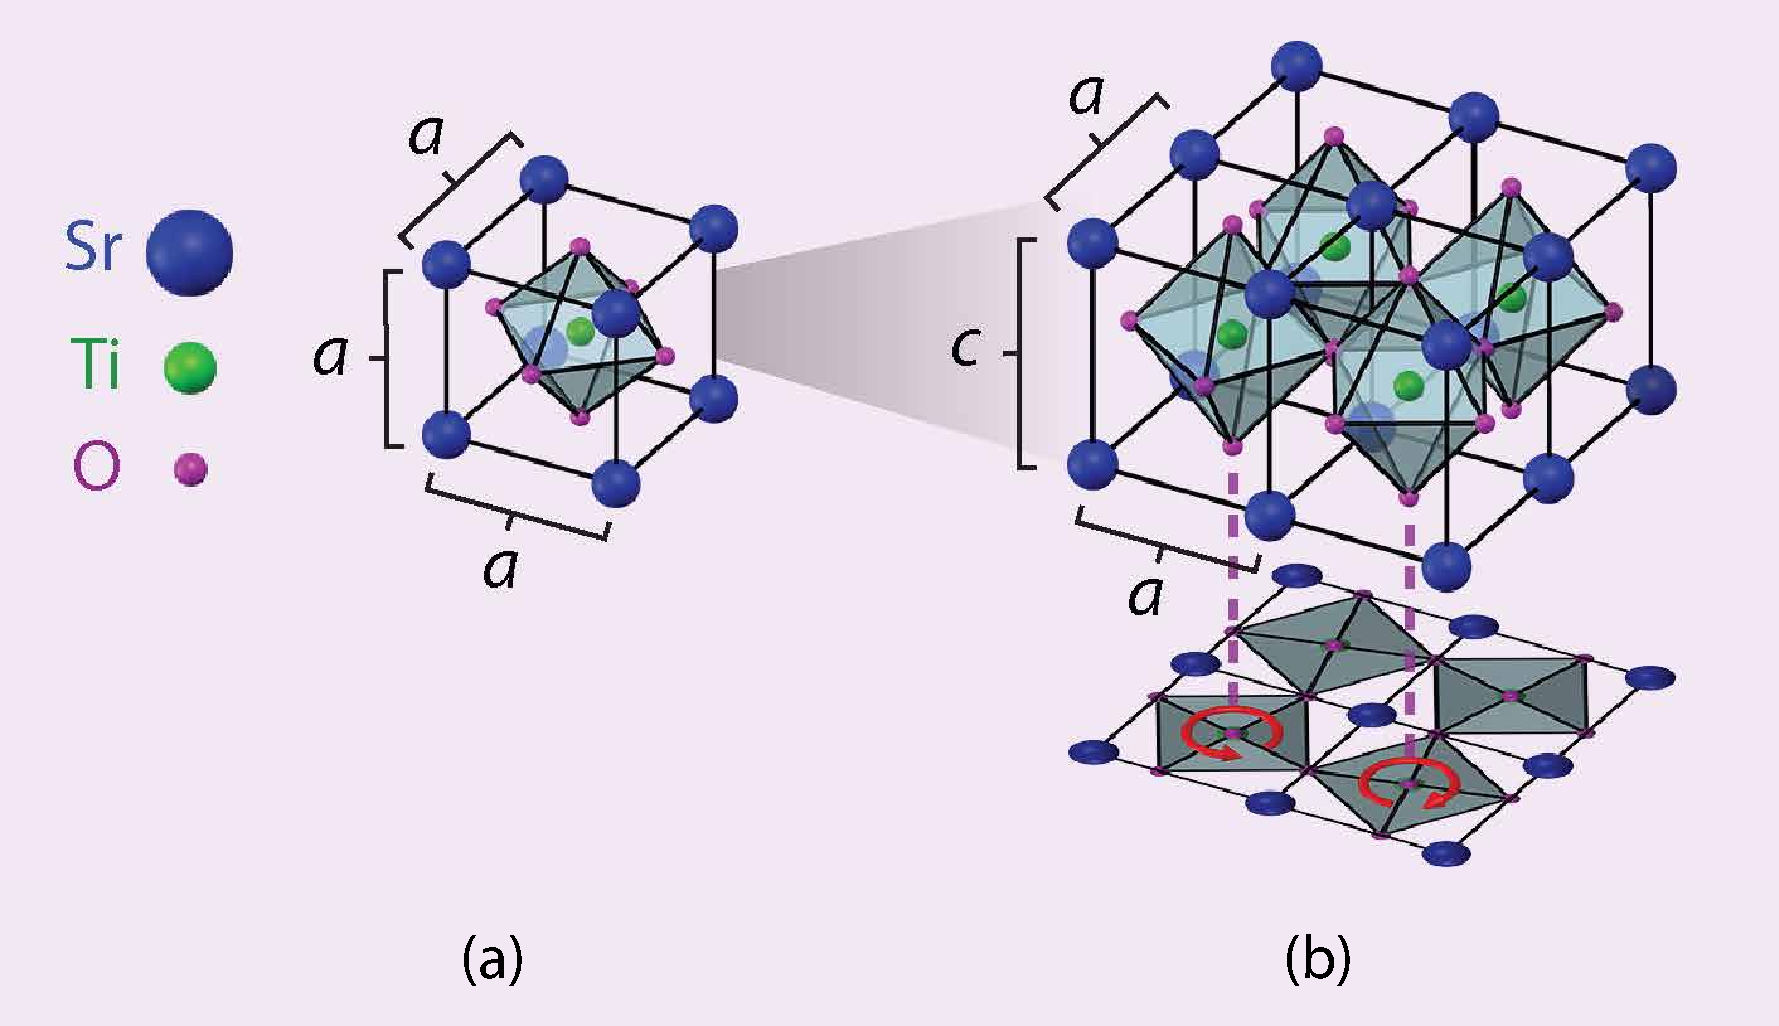
\includegraphics[width=.90\textwidth]{Drawing/STOPhaseTransition.pdf}
	\caption{Ferroelastic transition of STO. (a) At $T=300$ K STO has cubic perovskite structure. (b) At $T = 105$ K, the adjacent oxygen octahedrons would rotate in opposite directions and cause ferroelastic transition in STO. Domains will be formed for different orientations of unit cells. Adapted from \cite{sulpizio2014nanoscale}.}
	\label{FIG:STOPhaseTransition}
\end{figure}

At room temperature the STO is paraelectric, with a large dielectric constant ($\epsilon_r \sim 300$).  When the temperature is lower than $T=105$ K, the paraelectricity still persists. Although the elongation of unit cell in low temperature develops a double-well potential for Ti atoms, with potential minima at the oxygen at opposite sides of the the elongation axis, the Ti atoms do not displace towards the minima due to the quantum tunneling of oxygen atoms\cite{sulpizio2014nanoscale} between the minima. STO is one of the few materials that exhibit such \emph{quantum paraelectricity}\cite{muller1979srti}. As a result, the dielectric constant of STO increases rapidly with decreased temperature. The increase is also cut off by quantum tunneling, leaves $\epsilon_r \sim 20,000$\cite{sakudo1971dielectric}. This is especially important for gating experiment at low temperature, and more details will be discussed in the following chapters.

The band structure of STO is quite complex. As shown in Figure \ref{FIG:STOBand}, the conduction band is derived from the $3d$ titanium orbitals and the valence band is from the $2p$ oxygen orbitals. The degeneracy of the five $3d$ orbitals is broken by the crystal structure of STO, and then they are grouped into high energy bands $e_g$ (from $d_{3z^2 - r^2}$ and $d_{x^2-y^2}$), and low energy bands $t_{2g}$ (from $d_{xy}$, $d_{yz}$ and $d_{xz}$). Ti $d_{xy}$, $d_{yz}$ and $d_{xz}$ orbitals are coupled to neighboring identical orbitals through the $2p$ orbitals of oxygen atoms in between. Therefore, the hopping matrix elements for in-plane are much greater than than for out-of-plane. 

\begin{figure}[h!]
	\centering
	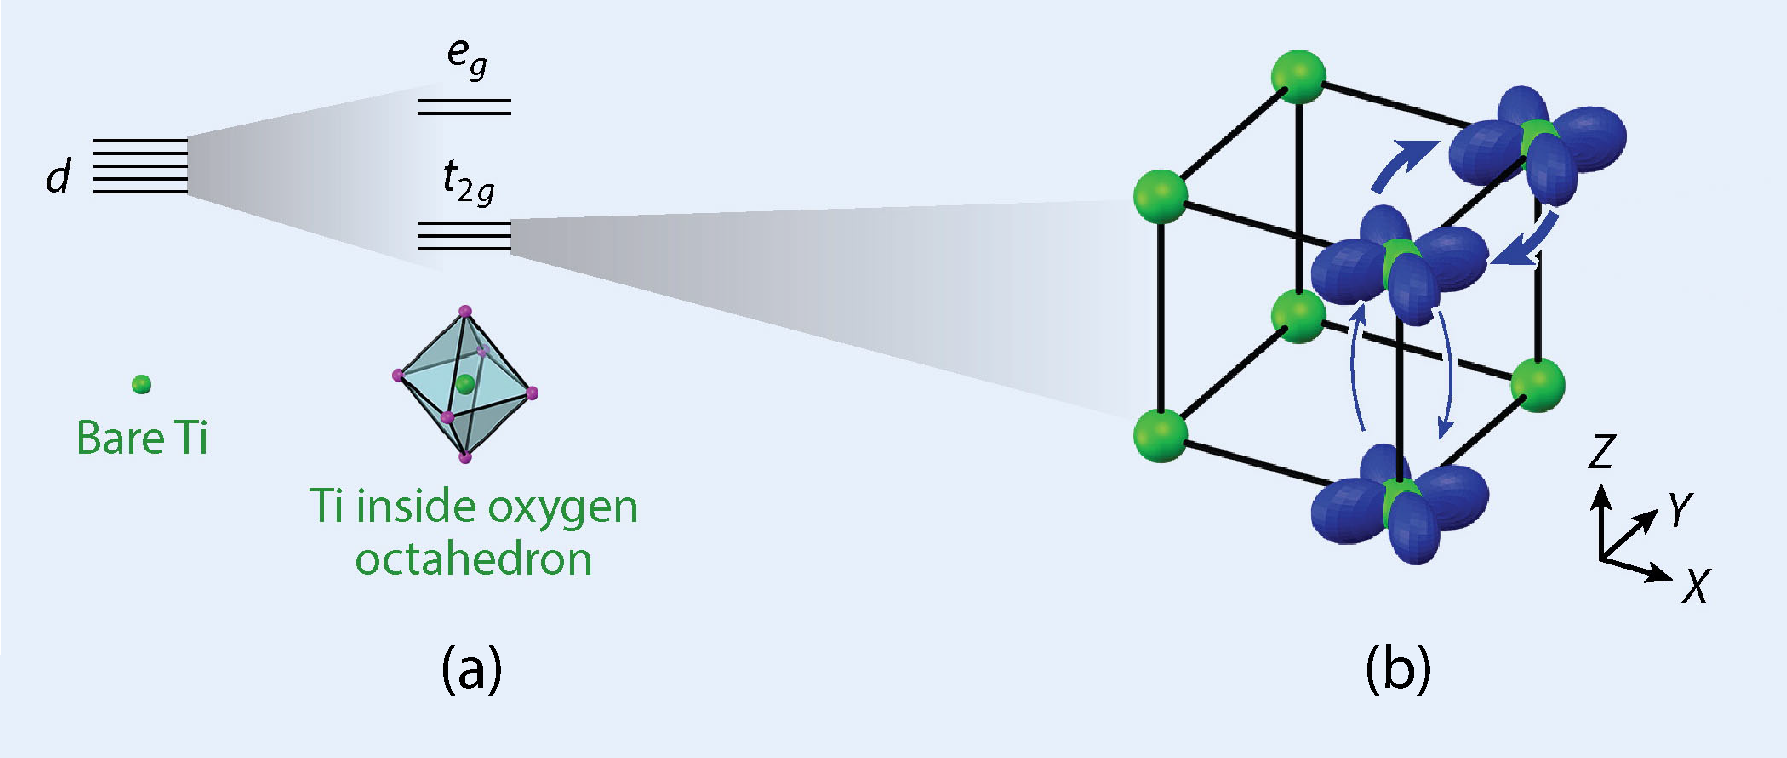
\includegraphics[width=.90\textwidth]{Drawing/STOBand.pdf}
	\caption{The band structure of bulk STO. (a) The conductive bands derive from the $3d$ orbitals of Ti. The degeneracy of the orbitals is broken by the octahedral cage of oxygen atoms, and the energy levels are grouped into $e_g$ and $t_{2g}$. (b) The hopping of $d_{xy}$, $d_{xy}$ and $d_{xy}$ are much easier along in the plane directions, mediated by the $2p$ orbitals of oxygen atoms. Adapted from \cite{sulpizio2014nanoscale}.}
	\label{FIG:STOBand}
\end{figure}

\subsection{2DEG on LAO/STO interface}

Although STO is a band insulator, when LAO is grown epitaxially (the small lattice mismatch of 3\% makes it possible) on TiO$_2$ terminated STO, the interface of LAO and STO becomes conductive and a layer of 2DEG is formed, first demonstrated by Ohtomo and Hwang in 2004\cite{ohtomo2004high}. The origin of interface 2DEG is still under debate. There are several different theories about the formation of 2DEG on the LAO/STO interface: polar catastrophe\cite{nakagawa2006some}, oxygen vacancy\cite{kalabukhov2007effect} and interfacial cation intermixing\cite{willmott2007structural}. 

The most widely accepted explanation is the polar catastrophe. Unlike the Ti$^{4+}$O$_2^{2-}$ and Sr$^{2+}$O$^{2-}$ planes in STO which are charge neutral, the La$^{3+}$O$^{2-}$ and Al$^{3+}$O$_2^{2-}$ layer are polar, with a net charge of $+e$ and $-e$ respectively. When LAO is grown on TiO$_2$ terminated STO, the polarity will generate a positive electric field, that builds up as the thickness goes up, as shown in Fig \ref{FIG:PolarCatastrophe}(a). To avoid the divergence of potential, the electrons are transferred from the surface to the interface and form 2DEG (Fig \ref{FIG:PolarCatastrophe}(c)). When LAO is grown on SrO terminated STO, a layer of hole gas will be formed in similar mechanism, as observed by Lee in 2018 \cite{lee2018direct}.
\\

\begin{figure}[h!]
	\centering
	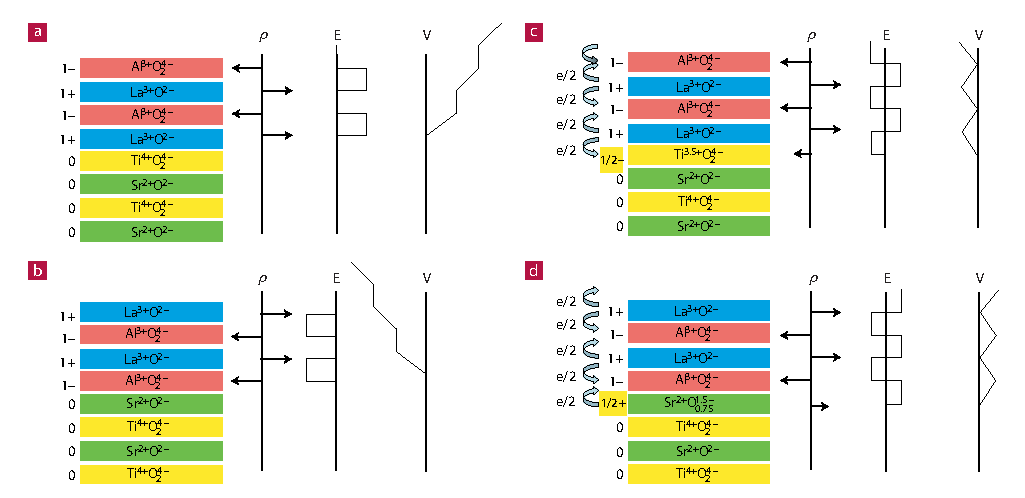
\includegraphics[width=1.0\textwidth]{Drawing/PolarCatastrophe.pdf}
	\caption{Polar catastrophe mechanism of interface conductivity of LAO/STO. (a) AlO$_2$ and LaO are not charge neutral and a non-zero potential is built up when LAO is grown on TiO$_2$ terminated STO. (c) Electrons are transferred from the top surface to neutralize the potential and therefore a layer of 2DEG is formed. (b) and (d) similar mechanism can explain the formation of hole gas on the interface. Adapted from \cite{nakagawa2006some}.}
	\label{FIG:PolarCatastrophe}
\end{figure}

However, there is a large discrepancy between the carrier density proposed by the polar catastrophe mechanism and measurement. In the polar catastrophe picture, each unit cell will donate half an electron, and result in carrier density of $3.2 \times 10^{14}$ cm$^{-2}$, while the observed values are in the order of $10^{13}$ cm$^{-2}$. Also, the formation of 2DEG on amorphous LAO on STO is contradicting to the polar catastrophe model. 

Oxygen vacancy is another possible explanation of the origin of 2DEG\cite{kalabukhov2007effect}, especially it is considered to be the source of conductivity of bulk STO\cite{schooley1965dependence}. Growth of LAO/STO sample under different oxygen partial pressure also shows that the carrier density is correlated to $P_{\mathrm{O_2}}$, therefore the oxygen vacancies can at least partially explain the formation of 2DEG. The magnetism is also considered related to the oxygen vacancies in STO, which will be discussed in future sections. There are also TEM\cite{nakagawa2006some} and XRD\cite{willmott2007structural} evidences support that cation intermixing across the interface can also explain the formation of 2DEG. The exchange of La$^{3+}$ and Sr$^{2+}$ provides extra electrons in the STO. However, this cannot explain the formation of hole gas formation with LAO grown on SrO terminated STO. So far, the polar catastrophe is the most widely accepted explanation of 2DEG in LAO/STO.

\subsection{Metal-insulator transition and critical thickness}

In 2006, Thiel et al.\cite{thiel2006tunable} reported that the interface of LAO/STO shows metal-insulator transition when the LAO is thicker than 4 unit cells. In Figure \ref{FIG:CriticalThickness}(a), when the thickness of LAO is over 4 u.c., the interface is conductive, otherwise the interface is insulating and the conductivity is below measurement limit. When LAO is slightly below the critical thickness (e.g. 3 u.c.), the conductivity on the interface is tunable, with a voltage applied to the backside of the sample. As Figure \ref{FIG:CriticalThickness}(b) demonstrates, when $V = +100$ V is applied, the interface becomes conductive. When the positive voltage is removed, the resistance is partially restored, but the interface is still conductive. However when $V = -100$ V is applied, the interface becomes insulating again. Similar phenomenon can be observed if the voltage is applied locally through a conductive AFM tip. More details are discussed in future chapters. 

\begin{figure}[p]
	\centering
	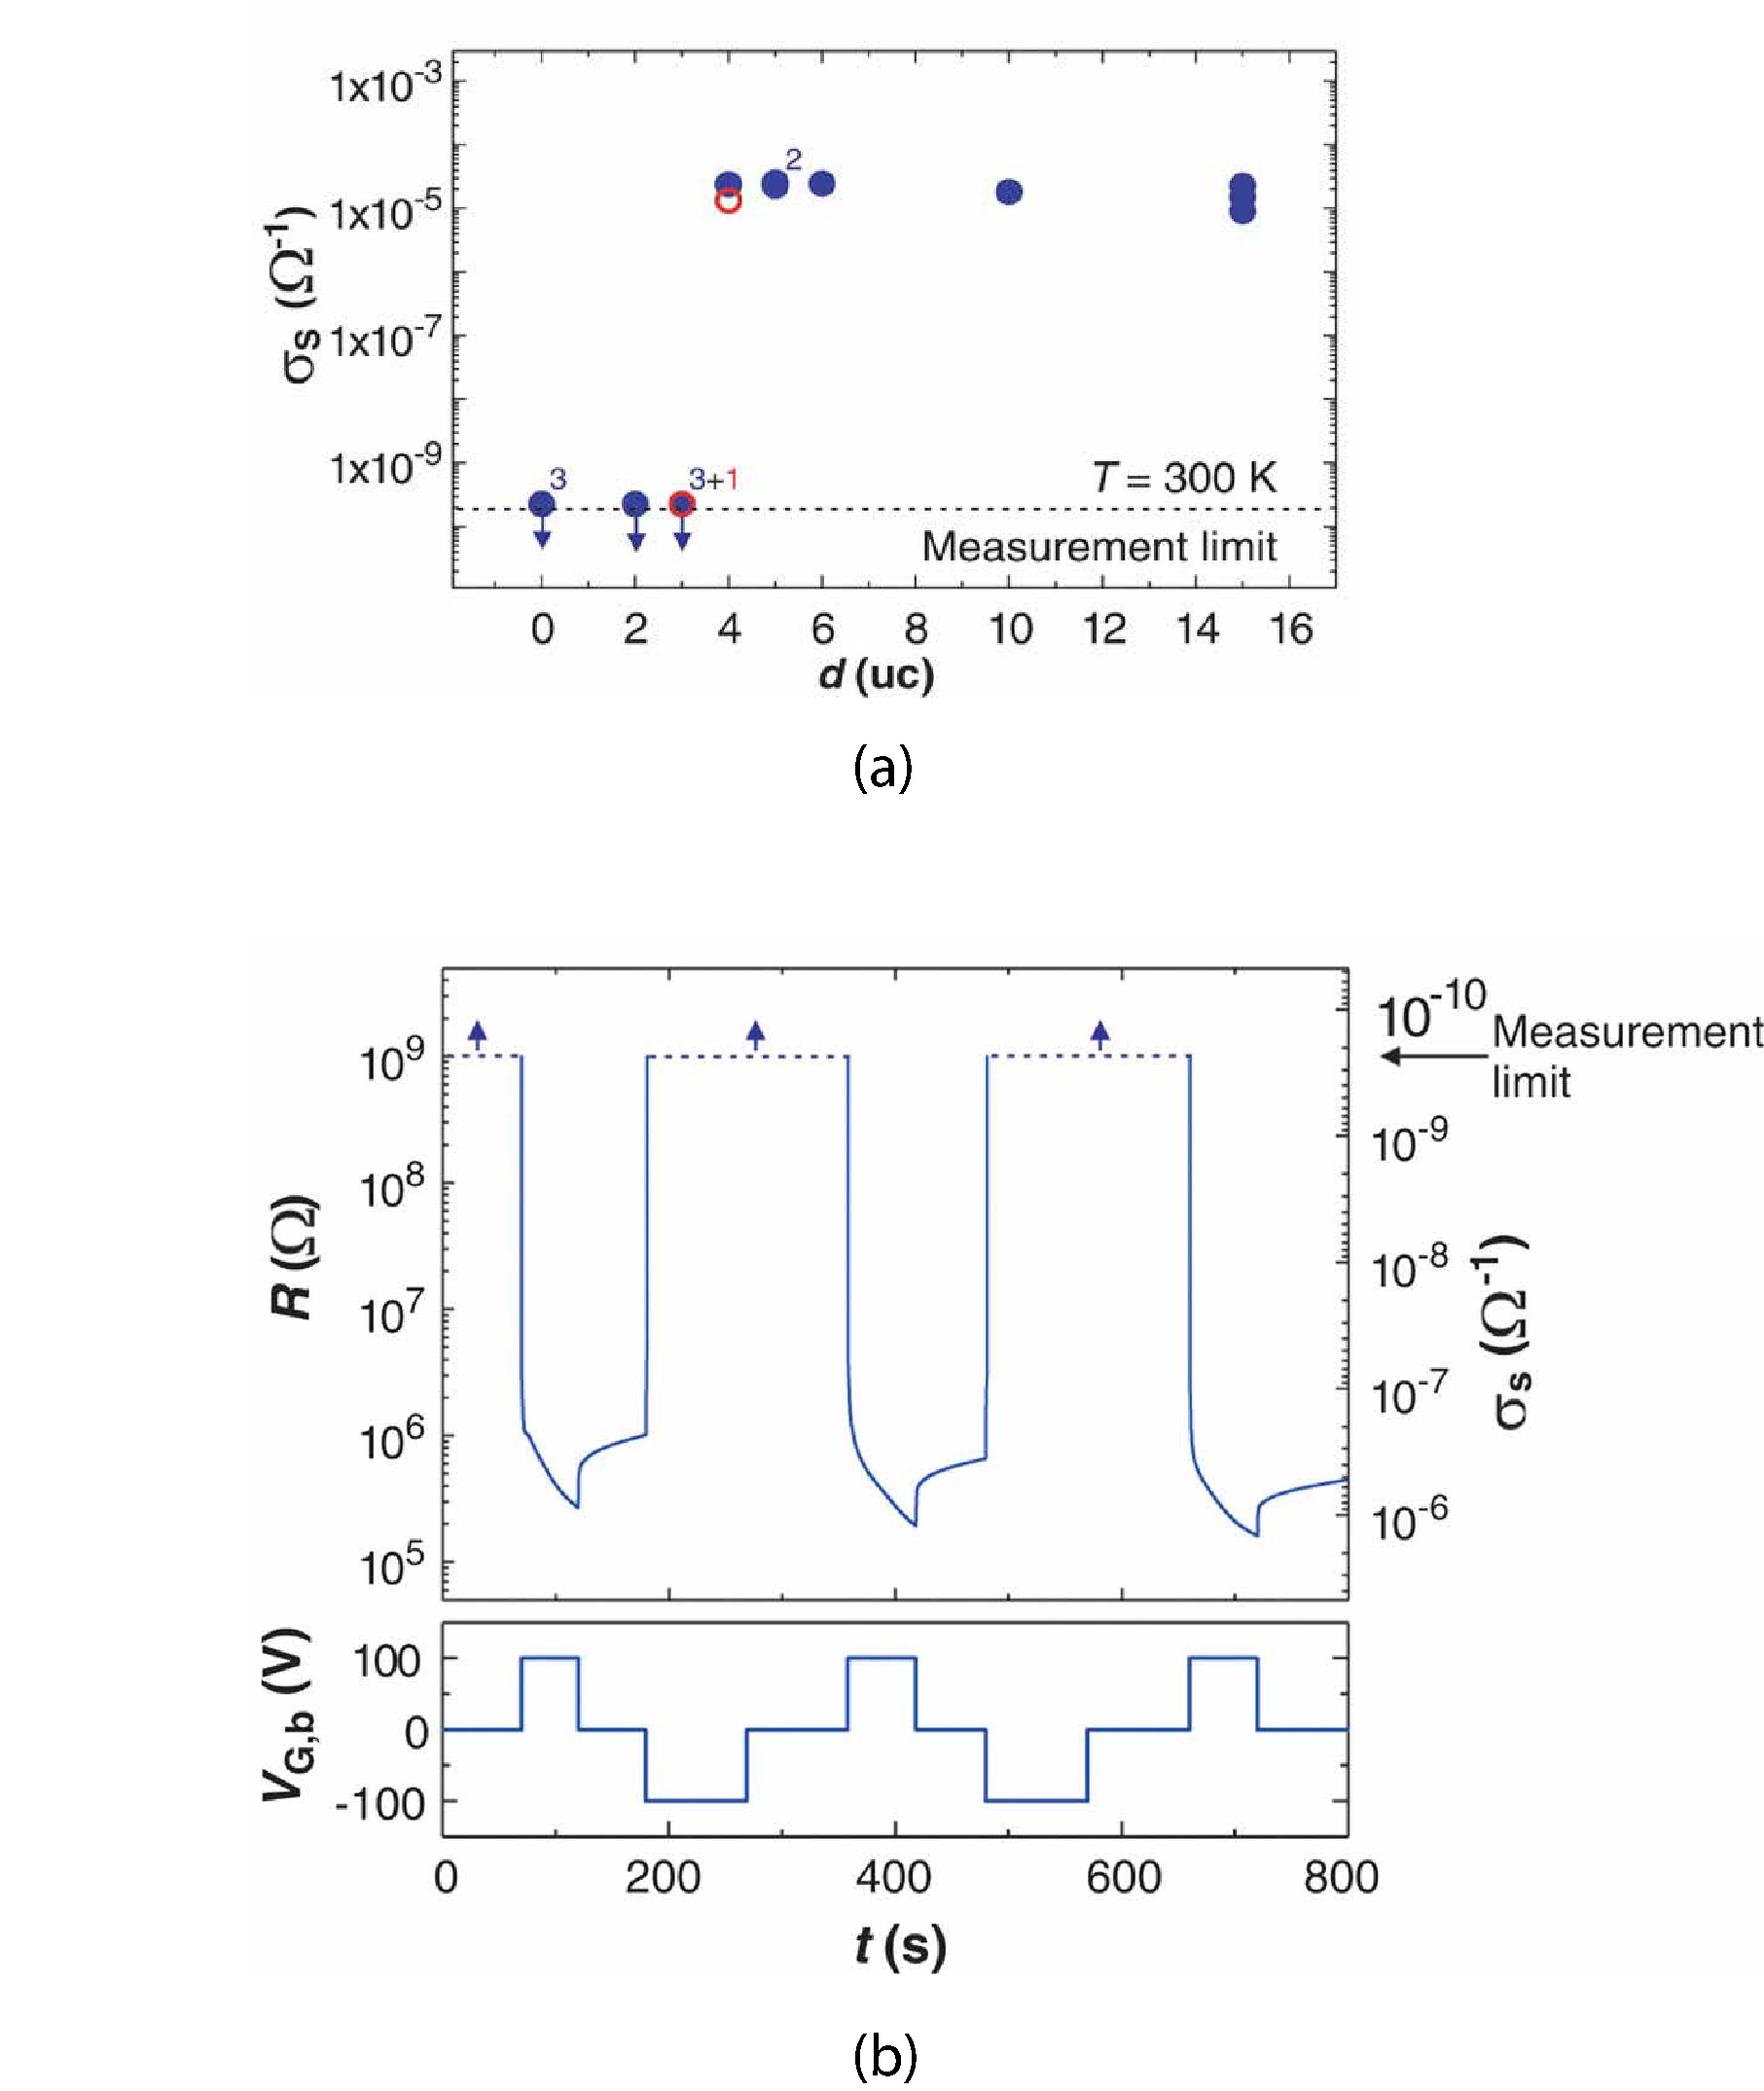
\includegraphics[width=0.7\textwidth]{Drawing/CriticalThickness.pdf}
	\caption{(a) When LAO is over the critical thickness of 4 unit cells, the interface is conductive, otherwise the interface is insulating. (b) When LAO is only slightly below the critical thickness (e.g. 3 unit cells), the conductivity on the interface is tunable with an external voltage applied to the backside. The as-grown sample is insulating. When $+100$ V is applied, the interface becomes conductive. When the voltage is removed, the conductivity still persists. When $-100$ V is applied, the interface becomes insulating again. The conductivity can by cycled with alternating voltages. Adapted from \cite{thiel2006tunable}.}
	\label{FIG:CriticalThickness}
\end{figure}

\subsection{c-AFM lithography of 2DEG and ``water-cycle'' mechanism}

Following the discovery of backgate tunable interface 2DEG, Cen et al demonstrated in 2008 that LAO/STO interface conductivity can also be induced with a gate voltage applied with a c-AFM tip on sample surface\cite{cen2008nanoscale}. For a 3 u.c. LAO/STO sample, the previously discussed polar catastrophe mechanism is not strong enough to reconstruct the band structure and form 2DEG on the interface. With gate voltage locally applied with a nanoscale AFM tip, positive charge can be transferred on the surface of LAO and build up a potential to cause polar catastrophe. The threshold voltage on the tip is about $V_\mathrm{thresh} \approx 6$ V\cite{cen2008nanoscale}. The with conductive channel created in this method is in the same order as the AFM tip, $\sim$ 10 nm. The process is reversible, and the positive charge can be removed with a negative voltage. An insulating gap can therefore be created on the nanowire. More experimental details are discussed in Section \ref{SEC:AFMLitho}.

The tunability of the LAO/STO with positive c-tip voltage can be explained with the ``water-cycle'' mechanism\cite{bi2010water}. The water adsorbed onto LAO surface is dissociated into OH$^{-}$ and H$^{+}$. A positively biased tip removes the OH$^{-}$ and leave excessive H$^{+}$ on LAO surface, which build up the polar catastrophe potential. In the erasing process, the negatively biased c-AFM tip removes the H$^{+}$ and restores OH$^{-}-H^{+}$ balance, and the interface becomes insulating. The water cycle mechanism is supported by the control c-AFM writing experiments performed in vacuum\cite{bi2010water}.

\begin{figure}[h!]
	\centering
	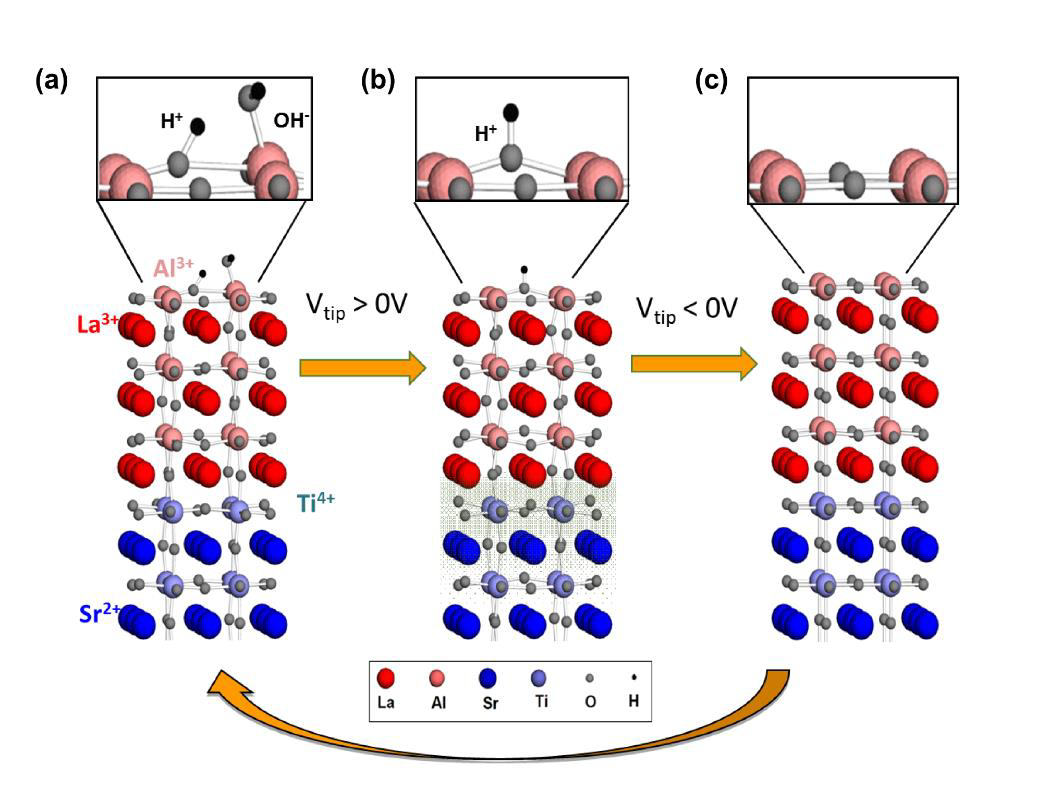
\includegraphics[width=0.8\textwidth]{Drawing/WaterCycle.png}
	\caption{A positively biased c-AFM tip removes removes the OH$^{-}$ and leave excessive H$^{+}$ on LAO surface, and the positive charges induce 2DEG on the interface underneath. A negatively biased c-AFM removes the H$^{+}$, and restores OH$^{-}-H^{+}$ balance. Adapted from Adapted from C. S. Hellberg's APS talk.}
	\label{FIG:WaterCycle}
\end{figure}

\subsection{Superconductivity}

Superconductivity has been found in STO since 1960s'\cite{schooley1964superconductivity}. Interface superconductivity on LAO/STO was first reported by Reyren et al in 2007\cite{reyren2007superconducting}, with a phase transition temperature $T_c$ of 200 mK. The in-plane and out-of-plane critical fields are around 1 T to 2 T and less than 1 T. Recently it was found that the electron pairing can persist up to a few T, much higher than the critical field of superconductivity, possible induced by strong correlation between electrons\cite{cheng2015electron}.

\subsection{Magnetism}

LAO and STO are both non-magnetic materials, however in 2007 the signature of magnetism was discovered on the interface from Kondo-like behavior of interface resistance \cite{brinkman2007magnetic}. More characterization of the interface magnetism were conducted with torque magnetometry\cite{li2011coexistence}, scanning quantum interference device (SQUID)\cite{bert2011direct}, and x-ray circular dichrism (XMCD)\cite{lee2013titanium}. In 2014, Feng et al found that the interface ferromagnetism is electronically tunable at room temperature, from MFM measurement\cite{bi2014room}. Optical measurements of the ferromagnetism will be discussed in Chapter \ref{SEC:Kerr}.

\section{Graphene}

Graphene is a single layer of carbon atom arranged in honey-comb structure and was first isolated and studied by Novoselov et al.\cite{novoselov2004electric}. It has proved to be a powerful and versatile platform for studying condensed matter phenomena due to the unique crystal structure and Dirac fermion behavior of electrons\cite{wilson2006electrons}. The Dirac cone band structure makes it possible to tune the carrier density continuously between electrons and holes. This duality of carriers in graphene results in many exotic properties of graphene, such as Klein tunneling\cite{allain2011klein, katsnelson2006chiral, young2009quantum, shytov2008klein}, edge state mixing\cite{williams2007quantum, abanin2007quantized, lohmann2009four, amet2014selective}, and recently the ``wedding cake'' structure of quantum Hall states\cite{gutierrez2018interaction}. Bandstructure engineering of graphene has been successful using moire pattern\cite{dean2013hofstadter, hunt2013massive}, interlayer interaction between twisted graphene\cite{cao2018correlated, cao2018unconventional} and external periodic electric fields\cite{forsythe2018band}. More exotic phases such as Hofstadter butterfly\cite{dean2013hofstadter, hunt2013massive, forsythe2018band}, Mott insulator\cite{cao2018correlated} and superconductivity\cite{cao2018unconventional} have been observed in graphene.

\subsection{Graphene band structure and Dirac fermion}

The band structure was first studied by Wallace et al. in 1947\cite{wallace1947band}. The orbital structure of C atom is $(1s)^2(2s)^2(2p)^4$. The $2s$ and $2p$ orbitals hybridize into $sp^2$ orbitals that form three $\sigma$ bonds with 120$^{\circ}$ angle, and a $\pi$ bond that provides free electrons. 

In in honey-comb lattice structure of graphene, there are two inequivalent sublattices that are mirror of each other, which can be labeled with $A$ and $B$. The Bravais lattice is hexagonal, and the primitive lattice vectors can be chosen to be: 
$$\mathbf{a_1} = \frac{a}{2}\left(3, \sqrt{3}\right), \ \ \ \mathbf{a_2} = \frac{a}{2}\left(3, -\sqrt{3}\right)$$

with $a = 1.42\mathrm{\AA}$ being the spacing between to adjacent C atoms. Using the relationship between the real space lattice and reciprocal lattice $\mathbf{a_i}\cdot\mathbf{b_j} = 2\pi\delta_{ij}$, the primitive reciprocal lattice vectors can be written as 
$$\mathbf{b_1} = \frac{2\pi}{3a}\left(1, \sqrt{3}\right), \ \ \ \mathbf{b_2} = \frac{2\pi}{3a}\left(1, -\sqrt{3}\right)$$

\begin{figure}[h!]
	\centering
	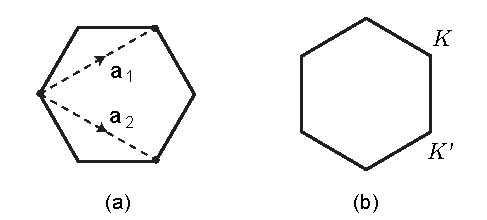
\includegraphics[width=0.7\textwidth]{Drawing/Bravais.pdf}
	\caption{(a) Primitive vectors of Bravais lattice. (b) First Brillouin zone of graphene.}
	\label{FIG:Bravais}
\end{figure}

The first Brillouin zone is also hexagonal shape. There are two types of corners, $K$ and $K'$, and their positions in the reciprocal space are:
$$\mathbf{K} = \frac{2\pi}{3a}\left(1, \frac{1}{\sqrt{3}}\right), \ \ \ \mathbf{K'} =  \frac{2\pi}{3a}\left(1, -\frac{1}{\sqrt{3}}\right).$$

The wavefunction of electron in graphene can be written as the superposition of states in the two sublattices $A$ and $B$:
$$\Psi(\mathbf{k}, \mathbf{r}) = \sum_{\alpha = A, B}c_{\alpha}(\mathbf{k}) \ \Phi_{\alpha}(\mathbf{k}, \mathbf{r}),$$
and the wavefunctions for the sublattice states can be written as Bloch wave functions:
$$\Phi_{\alpha}(\mathbf{k}, \mathbf{r}) = \frac{1}{\sqrt{n}}\sum_\mathbf{R} e^{-i \mathbf{k} \cdot \mathbf{R}} \ \phi_{\alpha}(\mathbf{r} - \mathbf{R}),$$
where $\phi_{\alpha}$ is the wavefunction at each atomic site, R is over the entire Bravais lattice, and $n$ is the number of unit cells in the crystal. 

The tight-binding model assumes that the hopping is only allowed for the nearest and next nearest neighbors, and therefore the Hamiltonian can be written as\cite{wallace1947band, neto2009electronic}:
\begin{equation}
\begin{split}
\mathbf{H} = & - t \sum_{ij=\mathrm{n.n.}, \ \sigma} (a_{i\sigma}^{\dagger} b_{j\sigma} + \mathrm{H. c.}) \\
& - t' \sum_{ij=\mathrm{n.n.n.}, \ \sigma} (a_{i\sigma}^{\dagger} a_{j\sigma} + b_{i\sigma}^{\dagger} b_{j\sigma} + \mathrm{H. c.}),
\end{split}
\label{EQN:Hamiltonian}
\end{equation}
where $t$ is the hopping energy, $a_{i\sigma}^{\dagger}$ is the creation operator for the state on the $i$th site of sublattice $A$ with spin $\sigma\in\{+1, -1\}$, and $b_{j\sigma}$ is the annihilation operator for state on the $j$th site of sublattice $B$ with spin $\sigma$. The summation is over all the nearest neighbors for the 1st term and next nearest neighbors for the 2nd term. For sublattice $A$, the three nearest neighbors in real-space are: 
$$\mathbf{\delta}_1 = \frac{a}{2}\left(1, \sqrt{3}\right), \ \ \ \mathbf{\delta}_2 =  \frac{a}{2}\left(1, -\sqrt{3}\right), \ \ \ \mathbf{\delta}_3 = -a(1, 0),$$
and the next nearest neighbors are:
$$\mathbf{\delta}'_1 = \pm \mathbf{a}_1, \ \ \ \mathbf{\delta}'_2 =  \pm \mathbf{a}_2, \ \ \ \mathbf{\delta}'_3 = \pm (\mathbf{a}_2 - \mathbf{a}_1).$$
The resulting eigen energies are\cite{wallace1947band, neto2009electronic}
$$E_{\pm}(\mathbf{k}) = \pm t \sqrt{3 + f(\mathbf{k})} - t'f(\mathbf{k}),$$
with
$$f(\mathbf{k}) = 2 \, \mathrm{cos}\left( \sqrt{3} k_y a \right) + 4 \, \mathrm{cos}\left(\frac{\sqrt{3}}{2} k_y a \right) \, \mathrm{cos}\left( \frac{3}{2} k_y a \right).$$
The plus sign is for the upper band and minus sign is for the lower band. 

For $\mathbf{k}$ close to $\mathbf{K}$ (or $\mathbf{K'}$), set $\mathbf{q} = \mathbf{K} - \mathbf{k}$, with $|\mathbf{q}| \ll |\mathbf{K}|$, then the band energies can be approximated by a linear dispersion relation
$$E_{\pm}(\mathbf{q}) \approx v_F|\mathbf{q}|,$$
with $\mathbf{q}$ being the momentum $\mathbf{k}$ relative to $\mathbf{K}$ (or $\mathbf{K'}$), and $v_F \approx c/300$ or $10^6$m/s. The Hamiltonian can be written as 
\begin{equation}
\mathbf{H}(\mathbf{q}) = 
\hbar v_F 
\begin{pmatrix}
0 & q_x + iq_y \\
q_x - iq_y & 0
\end{pmatrix}
=
\hbar v_F \hat{\mathbf{\sigma}} \cdot \mathbf{q}
\label{EQN:DiracHamiltonian}
\end{equation}
in the basis of \emph{sublattice states}, with the components of $\hat{\sigma}$ operator being the usual Pauli matrices. The eigenvectors for states around $\mathbf{K}$ and $\mathbf{K'}$ are
\begin{equation}
\psi_{\pm, \mathbf{K}}(\mathbf{q}) = \frac{1}{\sqrt{2}} 
\begin{pmatrix}
e^{-i\theta_{\mathbf{q}}/2} \\
\pm e^{i\theta_{\mathbf{q}}/2}
\end{pmatrix}, \ \ \
\psi_{\pm, \mathbf{K'}}(\mathbf{q}) = \frac{1}{\sqrt{2}} 
\begin{pmatrix}
e^{i\theta_{\mathbf{q}}/2} \\
\pm e^{-i\theta_{\mathbf{q}}/2}
\end{pmatrix}.
\label{EQN:Eigenstates}
\end{equation}
with 
$$\theta_\mathbf{q} = \mathrm{tan}^{-1}\left(\frac{q_x}{q_y}\right)$$
The plus and minus signs are corresponding to states in the conductance and valence bands. Notice that when $\mathbf{q}$ rotates around $\mathbf{K}$ (or $\mathbf{K'}$), the phase of $\psi_{\pm, \mathbf{K}}$ (or $\psi_{\pm, \mathbf{K'}}$) only changes by $\pi$ instead of $2\pi$. Therefore the sublattice states are also called ``pseudo-spin'' states\cite{neto2009electronic}. 

\begin{figure}[h!]
	\centering
	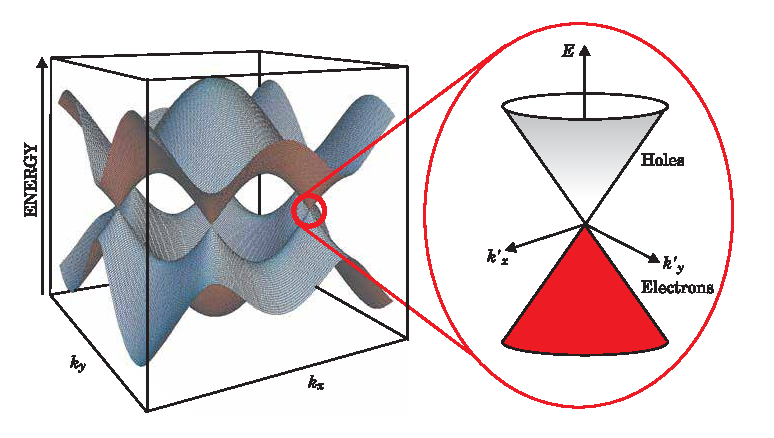
\includegraphics[width=0.8\textwidth]{Drawing/GrapheneBand.pdf}
	\caption{The band structure of Graphene. The low energy approximation around $\mathbf{K}$ and $\mathbf{K'}$ has linear dispersion relation. The conduction and valence bands are gapless and the electron behave like Dirac fermions. Adapted from \cite{wilson2006electrons}.}
	\label{FIG:GrapheneBand}
\end{figure}

A significant difference between graphene and normal semiconductor is that, the electron and hole states are described by the same wavefunction, and both are obtained from a Hamiltonian of the form of a relativistic particle described by the 2D Dirac equation\cite{neto2009electronic}. Therefore the electrons in graphene has the properties of Dirac fermions, such as handedness. Also notice that the spinors for $\mathbf{q}$ around $\mathbf{K}$ and $\mathbf{K'}$ differ by a phase of $\pi$ (equation \ref{EQN:Eigenstates}), therefore the states are opposite in handedness around $\mathbf{K}$ and $\mathbf{K'}$. However, at $\mathbf{K}$ and $\mathbf{K'}$ the wavefunctions are still the linear combination of the two sublattice states, or the pseudo-spin states. This degree of freedom will introduce extra degeneracies and will be discussed in the following section.

\subsection{Quantum Hall effect}

Quantum Hall effect is one of the most important discovery in physics in the 20th century. In the classical Hall effect, a Hall voltage will be built by in the transverse direction of current in magnetic field. In the quantum Hall effect however, the Hall voltage built up by the magnetic field is quantized. This section will start from the classical behavior of electron in magnetic field, and discuss the unique quantum Hall effect in graphene.

\subsubsection{Classical Hall effect}

In the classical Drude model, the electrons are colliding with scattering centers and the average velocity is zero without external electric field. When a field is applied, the drift velocity is 
\begin{equation}
\mathbf{v}_d = -\frac{e\mathbf{E}}{m}\tau,
\label{EQN:ClassicalE}
\end{equation}
where $\mathbf{E}$ is the external field, and $\tau$ is the mean free time between two collisions. The current density can be written as 
$$\mathbf{j} = -ne\mathbf{v}_d = \frac{ne^2\tau}{m}\mathbf{E},$$
where $n$ is the carrier density in the conductor. The conductivity is 
\begin{equation}
\sigma = \frac{\mathbf{j}}{\mathbf{E}} = \frac{ne^2\tau}{m} = n\mu e
\label{EQN:Conductivity}
\end{equation}
and $\displaystyle \mu \equiv \frac{e\tau}{m}$ is the mobility of carrier, which defines how fast the carriers move through a conductor. Usually when the scattering is less likely to happen, the mobility will be higher.

When a magnetic field is applied, the motion equation \ref{EQN:ClassicalE} is modified as 
\begin{equation}
\frac{m\mathbf{v}}{\tau} = -e(\mathbf{E} + \mathbf{v} \times \mathbf{B}).
\label{EQN:ClassicalEB}
\end{equation}
Assume the motion is in $x$-$y$ plane. The Ohm's law can be written as tensor form:
$$
\mathbf{j} = 
\mathbf{\sigma} \cdot \mathbf{E} =
\begin{pmatrix}
\sigma_{xx} & \sigma_{xy} \\
\sigma_{yx} & \sigma_{yy}
\end{pmatrix}
\begin{pmatrix}
E_{x} \\
E_{y}
\end{pmatrix}.
$$
The conductivity tensor $\mathbf{\sigma}$ can be solved using the motion equation \ref{EQN:ClassicalEB} and the definition of $\mathbf{\sigma}$ and $\mathbf{j}$:
$$
\mathbf{\sigma} = \frac{\sigma_0}{1 + \omega_c^2\tau^2}
\begin{pmatrix}
1 & -\omega_c\tau \\
\omega_c\tau & 1
\end{pmatrix},
$$
where $\sigma_0$ is the conductivity without magnetic field, and $\displaystyle \omega_c \equiv \frac{eB}{m}$ is the cyclotron frequency. The resistivity tensor can be calculated from $\mathbf{\sigma}$:
\begin{equation}
\rho_{xx} = \frac{1}{n\mu e}, \ \ \ \rho_{xy} = -\frac{B}{n e} = R_H B,
\label{EQN:Hall}
\end{equation}
with the Hall coefficient $\displaystyle R_H = -\frac{1}{ne}.$
The longitudinal resistivity $\rho_{xx}$ and transverse resistivity $\rho_{xy}$ are used to measure the carrier density and type $n$ and mobility $\mu$.

\subsubsection{Quantum Hall effect of Graphene}
\label{SEC:QuantumHall}

At low temperature and high magnetic field, the Hall resistance $R_{xy}$ is quantized into plateaus 
$$
R = \frac{1}{\nu}R_k = \frac{h}{\nu e^2},
$$
where $R_k = h/e^2 \approx 25812$ $\Omega$ is the von Klitzing constant, and the longitudinal resistance $R_{xx}$ is suppressed. The conductivity tensor becomes
$$ \displaystyle
\rho = 
\begin{pmatrix}
0 & \frac{\nu e^2}{h} \\ 
-\frac{\nu e^2}{h} & 0
\end{pmatrix}
$$

The quantum Hall effect can be understood semi-classically. In magnetic field, only the energy levels correspond to the quantized cyclotron orbits with integer flux are allowed:
$$E = \hbar\omega_c \left(n + \frac{1}{2}\right),$$
where $\omega_c$ is the cyclotron frequency and the orbitals are called Landau Levels.

The electrons that carry the current flow near the edge, while bouncing against the boundary and form chiral edge current channels. The backscattering is suppressed by the magnetic field, and therefore $R_{xx} = 0$ when the Fermi energy is between two Landau levels. The electrons in the bulk of the 2D conductor are trapped in the localized states induced by the scattering centers. When the Fermi energy is elevated to the next Landau level, the electrons start to fill the new localized states and the longitudinal resistance will be non-zero, while the Hall resistance transits to another plateau.

In graphene, the quantum Hall behavior was first observed by Novoselov et al.\cite{novoselov2005two} and Zhang et al.\cite{zhang2005experimental} in 2005. The Hall conductance follows
$$
\sigma_{xy} = \pm 4\left(n + \frac{1}{2}\right)\frac{e^2}{h}.
$$
The 4 is from the degeneracy of two spin degree of freedom and two pseudo-spin degree of freedom. The half-integer is the result Berry phase of electrons\cite{zhang2005experimental} in graphene.

\begin{figure}[p]
	\centering
	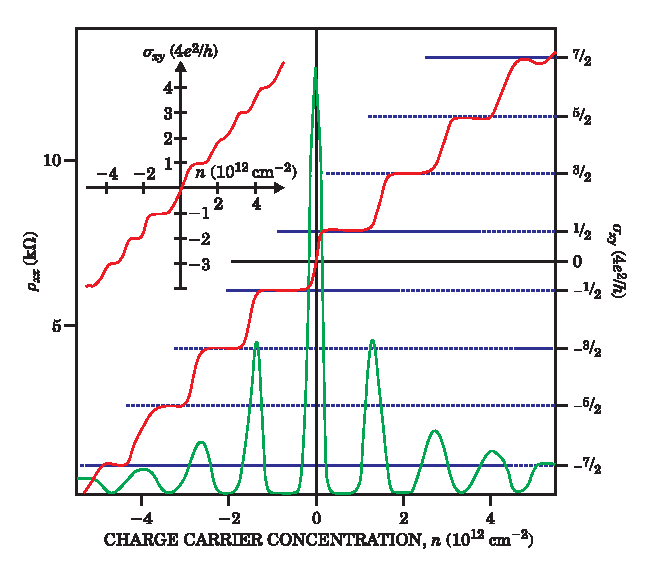
\includegraphics[width=0.8\textwidth]{Drawing/GrapheneQuantumHall.pdf}
	\caption{The quantum Hall effect in graphene. The Hall conductance (red line) follows $\displaystyle \sigma_{xy} = \pm4\left(n + \frac{1}{2}\right)\frac{e^2}{h}$, while the longitudinal resistance (blue line) shows peaks when the Fermi energy transits from one Landau level to another. Adapted from \cite{novoselov2005two}.}
	\label{FIG:GrapheneQuantumHall}
\end{figure}


\chapter{Experimental Methods}

\section{Sample growth}

\subsection{LAO/STO growth}
The properties of LAO/STO interfaces is extremely sensitive to growth conditions such as substrate temperature, background oxygen pressure, annealing conditions, etc\cite{}. The samples in my experiments are grown with pulsed laser deposition (PLD) by our collaborators at University of Wisconsin-Madison.

\subsubsection{Pre-growth treatment}

STO (001) substrates are purchased from commercial crystal suppliers. The substrates have a carefully controlled mis-cut angle $< 0.1^{\circ}$, so that the width atomic terraces on STO surface is about 500nm (Figure \ref{FIG:RHEED}(a)). It has been reported that the terraces on LAO/STO surface can affect the properties of the LAO/STO interface\cite{}, therefore I would like to place the nano-devices on a single terrace. If the terraces are too wide however, the LAO cannot grow evenly on STO surface during the PLD process due to the high activation energy for atomic migrations, and end up forming holes on the sample (FIG. \cite{}). 

Before PLD growth, the STO (001) substrates are etched with buffered HF acid to remove SrO and become TiO$_2$ terminated. Then they are annealed at $1000^{\circ}$C for several hours, so that the surface will reconstruct and form crystal terraces\cite{}. Then the samples are etched in HF acid for a second time for a clean surface to start with. 

\subsubsection{PLD deposition}

In PLD deposition, KrF excimer laser ($\lambda = 248$ nm) pulses are focused on a LAO target and plumes of target material are deposited on the pre-heated STO substrates. Two growth conditions are used for LAO/STO samples: (a) STO substrate is heated at $T_\mathrm{STO} = 550^{\circ}$C and chamber background oxygen pressure $P(O_2)$ is maintained at $1 \times 10^{-3}$ mbar, and sample is annealed in 1 atm of $O_2$ after growth. (b) STO substrate is heated at $T_\mathrm{STO} = 780^{\circ}C$ and chamber background oxygen pressure $P(O_2) = 7.5 \times 10^{-5}$ mbar; sample is annealed at $T_\mathrm{STO} = 600^{\circ}$C, $P(O_2) = 300$ mbar for 1 hour after growth, or the so called ``Augsburg condition''. Samples grown in condition (a) are used for nano-scale device lithography (i.e. the sub-critical thickness 3.4 uc LAO/STO samples), while condition (b) favors the formation of oxygen vacancies and sample grown in such conditions are used for magnetism experiments\cite{}. 

\begin{figure}[p]
	\centering
	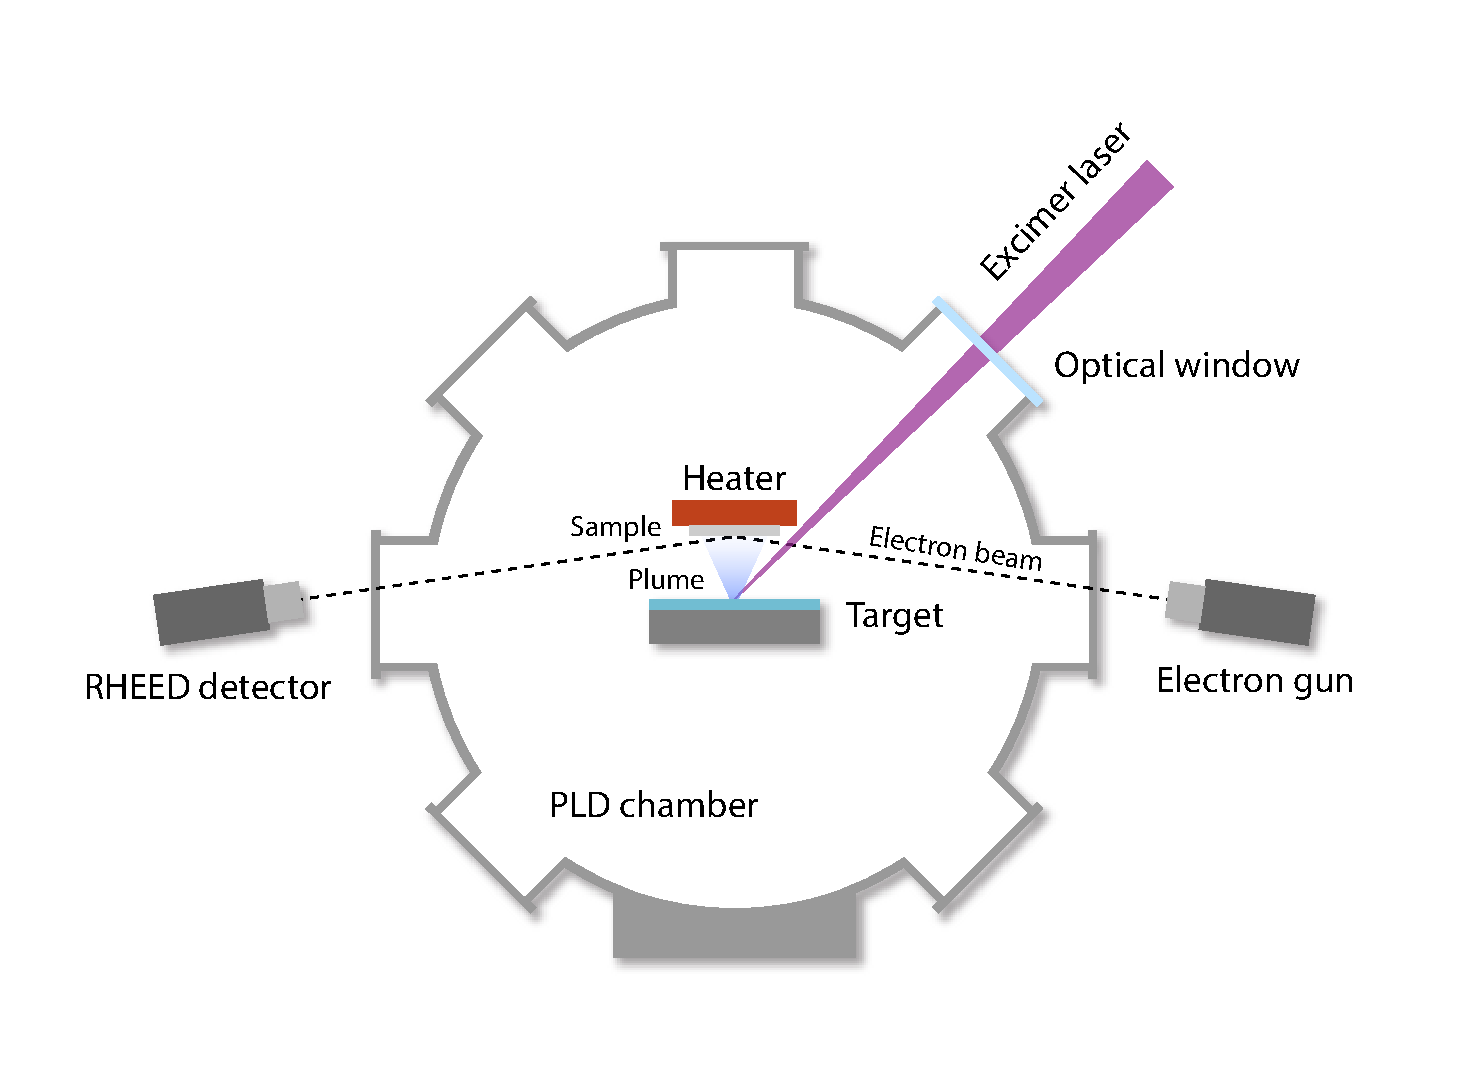
\includegraphics[width=1.0\textwidth]{Drawing/PLD.pdf}
	\caption{PLD epitaxial growth. The PLD chamber is back-filled with oxygen to the target pressure. A beam of pulsed deep-UV excimer laser is focused onto the LAO target. LAO is ablated off and a plume of plasma extends towards the heated substrate on top, and condensed into atomic layer films. RHEED signal is used to monitor the thickness of LAO.}
	\label{FIG:PLD}
\end{figure}

Figure \ref{FIG:PLD} illustrates PLD epitaxial growth of LAO. The sample is loaded in an ultra-high vacuum chamber, backed filled with oxygen to the target pressure. Deep UV excimer laser is focused on the LAO crystal target through an optical window on the chamber. The target material is ablated off by the laser and forms a plasma plume. The STO substrate is heated up and placed on top of the target. As the plume expands, target material would condense on the substrate and forms atomic-thin films epitaxially. The high temperature of the substrate facilitates crystallization and epitaxial growth of the target material. 

During the PLD growth, the reflection high-energy electron diffraction (RHEED) is used for \emph{in-situ} monitoring the thickness of epitaxial layers. A beam of electron is generated from a source and reflected from the substrate as the film growth. Electron diffraction signal is collected by a detector on the other side (Figure \ref{FIG:RHEED}(a) inset). The intensity of the diffraction oscillates as a function of film thickness. The thickness of LAO can be precisely controlled by counting the cycles of RHEED signal (Figure \ref{FIG:RHEED}(b)).

\begin{figure}[hp!]
	\centering
	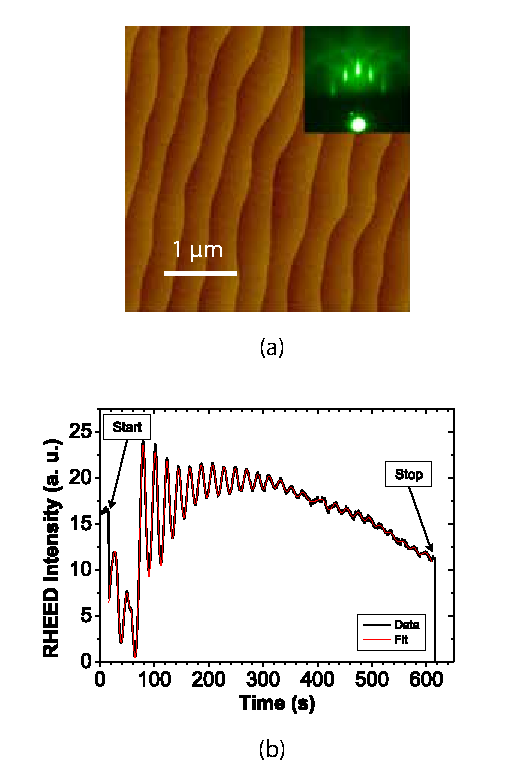
\includegraphics[width=0.7\textwidth]{Drawing/PLD_RHEED.pdf}
	\caption{AFM image of the sample after PLD growth and RHEED signal for PLD. (a) shows is the AFM Image. The stripes are the crystal terraces, with $h \approx 4 \mathrm{\AA}$. Inset of a is the raw diffraction sigal of RHEED. (b) is the RHEED signal oscillation during the film epitaxial growth. Each cycle indicates the completion of one unit cell. Adapted from \cite{podkaminer2016real}.}
	\label{FIG:RHEED}
\end{figure}

\subsection{Graphene growth}

The two most popular methods to obtain single-layer/few-layer graphene are mechanical exfoliation and chemical vapor deposition (CVD). 

The mechanical exfoliation isolate single layer graphene directly with adhesive tapes. Graphene is a type of Van der Waals material, which means that the carbon atoms within a layer are tightly bonded with covalent bond while the layers are bonded by the much weaker Van der Waals force. Adhesive tapes can easily separate graphene layers. After multiple exfoliation steps, single layer graphene flakes can be separated and identified\cite{}. One key aspect of the exfoliation method is choosing a proper substrate so that single layer graphene can be easily identified with optical microscopes. Although graphene has the highest absorption coefficient in the visible light regime\cite{}, spotting a single layer graphene flake on a transparent substrate is still challenging, and is always assisted with other characterization methods such as Raman spectroscopy\cite{} to ensure the graphene is single layer. The most commonly used substrate is silicon wafer with 400 nm thick silicon oxide coating. The graphene on SiO$_2$ surface modifies the interference of visible light between the top and bottom layer of the coating, and make graphene layers distinguishable\cite{}. 

CVD is another method to obtain single layer graphene. Graphene flake from mechanical exfoliation is mostly a few micrometers or tens of micrometers; the size and shape cannot be well controlled. CVD on the other hand, can grow continuous graphene of wafer sizes\cite{}, and then etch it into any desired shapes through post processing. 

The CVD process uses gaseous organic molecules (methane, ethylene, etc) as carbon source, and graphene lattice-matching crystal such as SiC, Ni and Cu as substrate. In high temperature (about 1000 $^{\circ}$C), the metal surface has highly reactive and can serve as a catalyst, so the gas molecules will react with the surface and carbon atoms are detached. At the high temperature, the carbon atoms will self-assemble into graphene. Over the entire process the substrate is in continuous gas flow so the gaseous byproducts are flushed away. Hydrogen is used to assist the growth. Without hydrogen molecules, graphene will grow simultaneously on the entire surface and form many small domains. Hydrogen will etch away the smaller domains while the larger domains are growing\cite{} until the domains meet or the process is terminated. If the hydrogen portion is too high however, the larger graphene domains will also be etched. CVD is a dynamic process of etching and growth. The ratio of methane and hydrogen need to be carefully controlled.

\begin{figure}[h!]
	\centering
	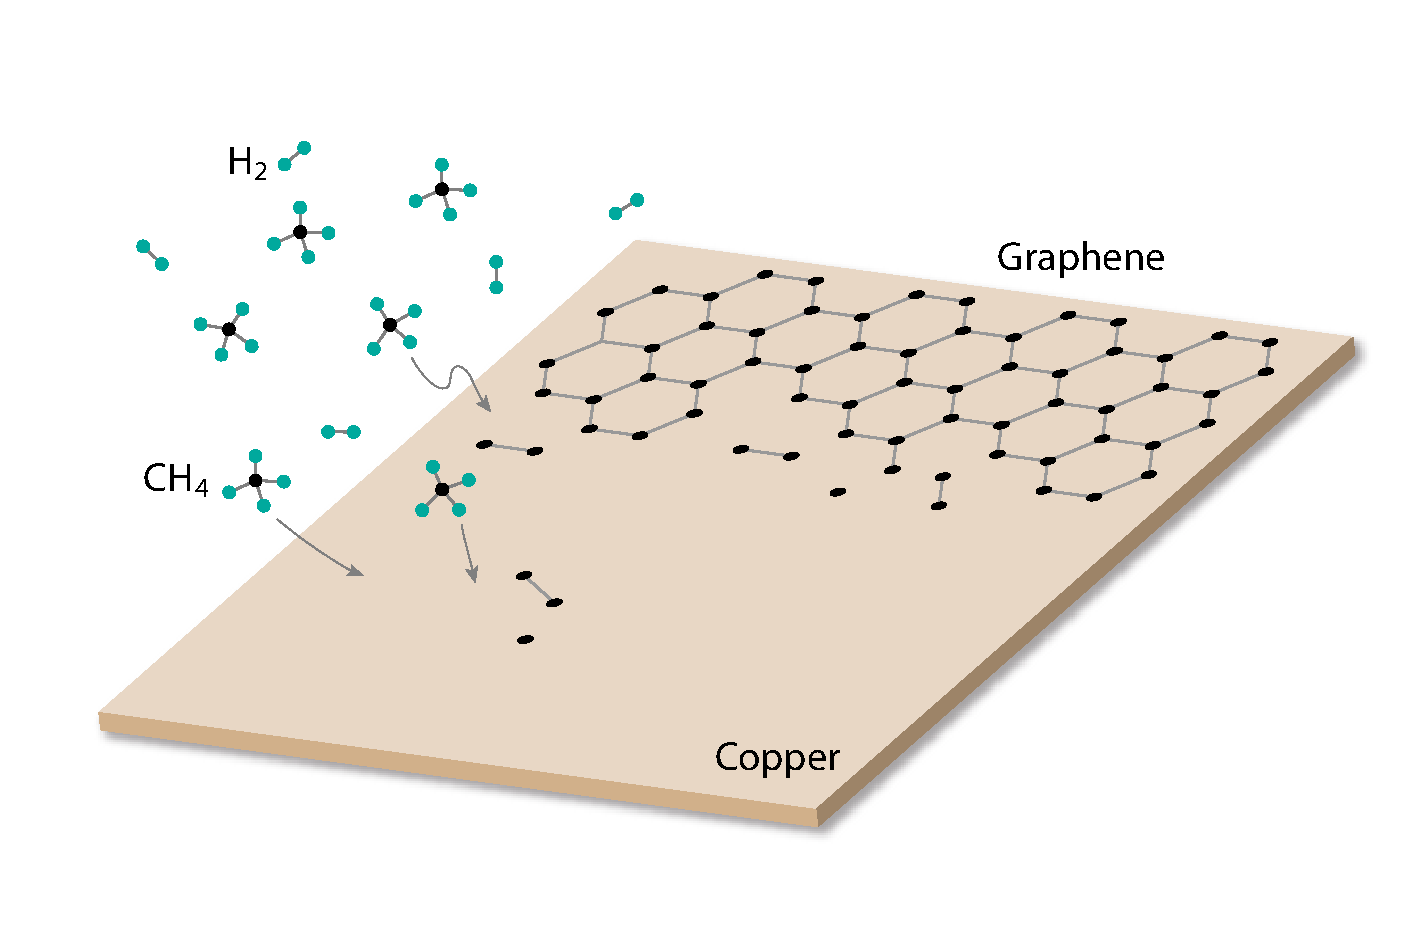
\includegraphics[width=.90\textwidth]{Drawing/CVD.pdf}
	\caption{Graphene CVD growth. At a temperature $T \approx$ 1000 $^{\circ}$C, methane molecules will react with copper surface and leave carbon atom on the surface. Carbon atom will self-assemble into graphene due to lattice-match between graphene and copper super-cell. Hydrogen is used to etch away the smaller domain so that the final single layer graphene domains is as large as possible. If the hydrogen is too much, the larger domain will be etched as well. Ratio of methane and hydrogen has to be carefully controlled.}
	\label{FIG:CVD}
\end{figure}

\subsubsection{Copper substrate preparation}

Various materials are used for graphene growth, most commonly SiC, Ir, Ni and Cu. Cu is the most common choice due to the low carbon solubility scalability\cite{Bae2010}. Compared to other substrate materials, copper is also easy to be etched with wet chemicals. In CVD growth, the carbon atoms form into graphene following the shape of the substrate. Therefore, the graphene quality is directly related to the substrate. Surface roughness and contaminants on copper provide nucleation centers for graphene, and can cause polycrystalline structure and multi-layer growth\cite{eres2014cooperative}. The issue of surface roughness can be addressed with electrochemical polishing\cite{Bae2010}, or mechanical polishing. In my experiment I used a graphene substrates polishing procedure developed by Dr Brian D'Urso's graduate students, by using diamond turning machine to reduce the roughness from several hundred of nanometer to a few nanometers\cite{dhingra2014chemical}. Compared to electrochemically polished substrates, this method can produce surface 50 time smoother and the copper domain sizes are 5 time larger. 

Diamond turning machine (DTM) is commonly used for high precision manufacturing, such as laser reflective mirrors. The DTM works like a lathe, where the workpiece is fixed on a turning spindle, and the cutting tool approaches the workpiece and shape or polish the surface by steps. Figure \ref{FIG:DTM} shows the DTM at work. The cylindrical metal piece in \ref{FIG:DTM}(a) is the spindle of DTM. Copper piece is fixed on the spindle by vacuum and spins at 2000 rpm. The diamond tool approaches the copper surface from the opposite side.  \ref{FIG:DTM}(b) is an image taken in the middle of a cutting step. Mineral spirit is sprayed from a nozzle from the left, cools down the surface and blow away the metal debris to the right. Reflection of the tool shows a flat finishing.

\begin{figure}[h!]
	\centering
	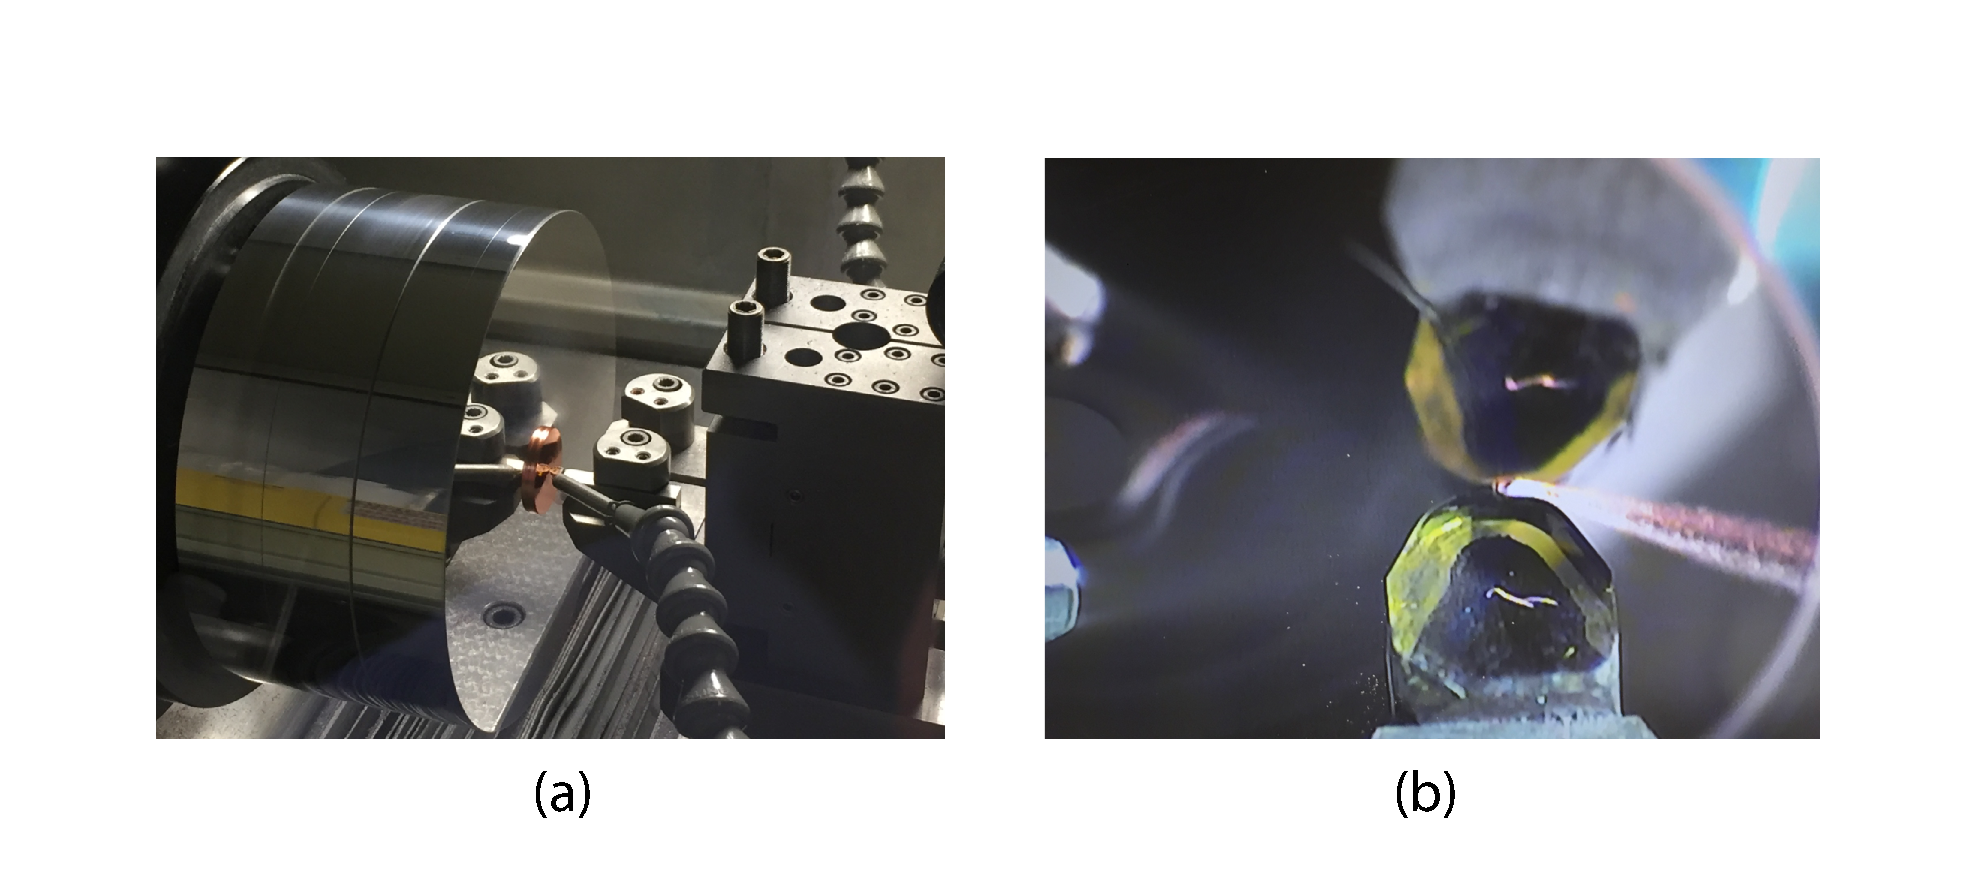
\includegraphics[width=1.0\textwidth]{Drawing/DTM.pdf}
	\caption{Diamond turning machine at work. (a) Copper is fixed onto a turning spindle with vacuum. (b) Mineral spirit is sprayed to the tool and cutting spot, to cool down the surface and blow away the debris.}
	\label{FIG:DTM}
\end{figure}

Instead of using high-speed-steel tool, the DTM uses a curved-edge (radius of curvature $r$ = 1.5 mm) diamond tool for cutting (Figure \ref{FIG:DiamondTool}). By reducing the incremental step to 10 $\mu$m, as shown in Figure \ref{FIG:DTMFinishing}, the roughness of the finishing surface can be smaller than 2 nm. The diamond tool sometimes have dents on the surface, which can leave a trace after each revolution.

\begin{figure}[h!]
	\centering
	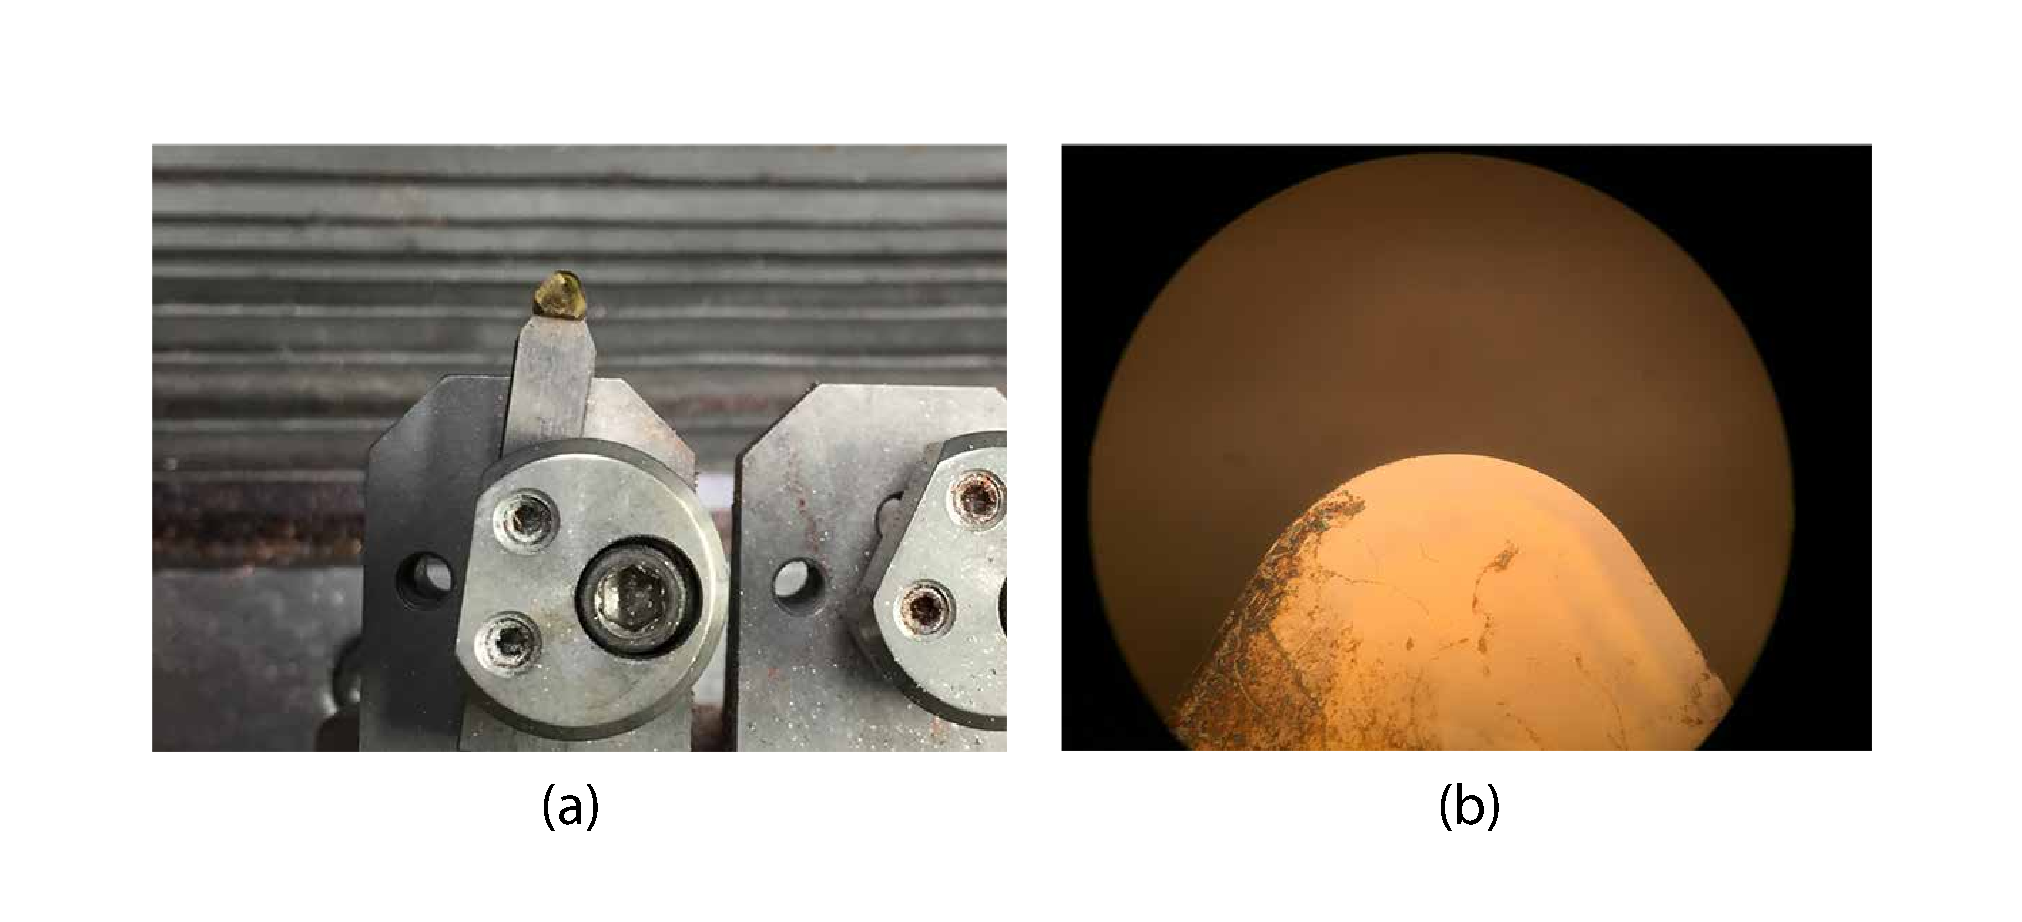
\includegraphics[width=1.0\textwidth]{Drawing/DiamondTool.pdf}
	\caption{(a) Diamond cutting tool. (b) Magnified image of the tool tip. The radius of curvature $r = 1.5$ mm.}
	\label{FIG:DiamondTool}
\end{figure}

\begin{figure}[h!]
	\centering
	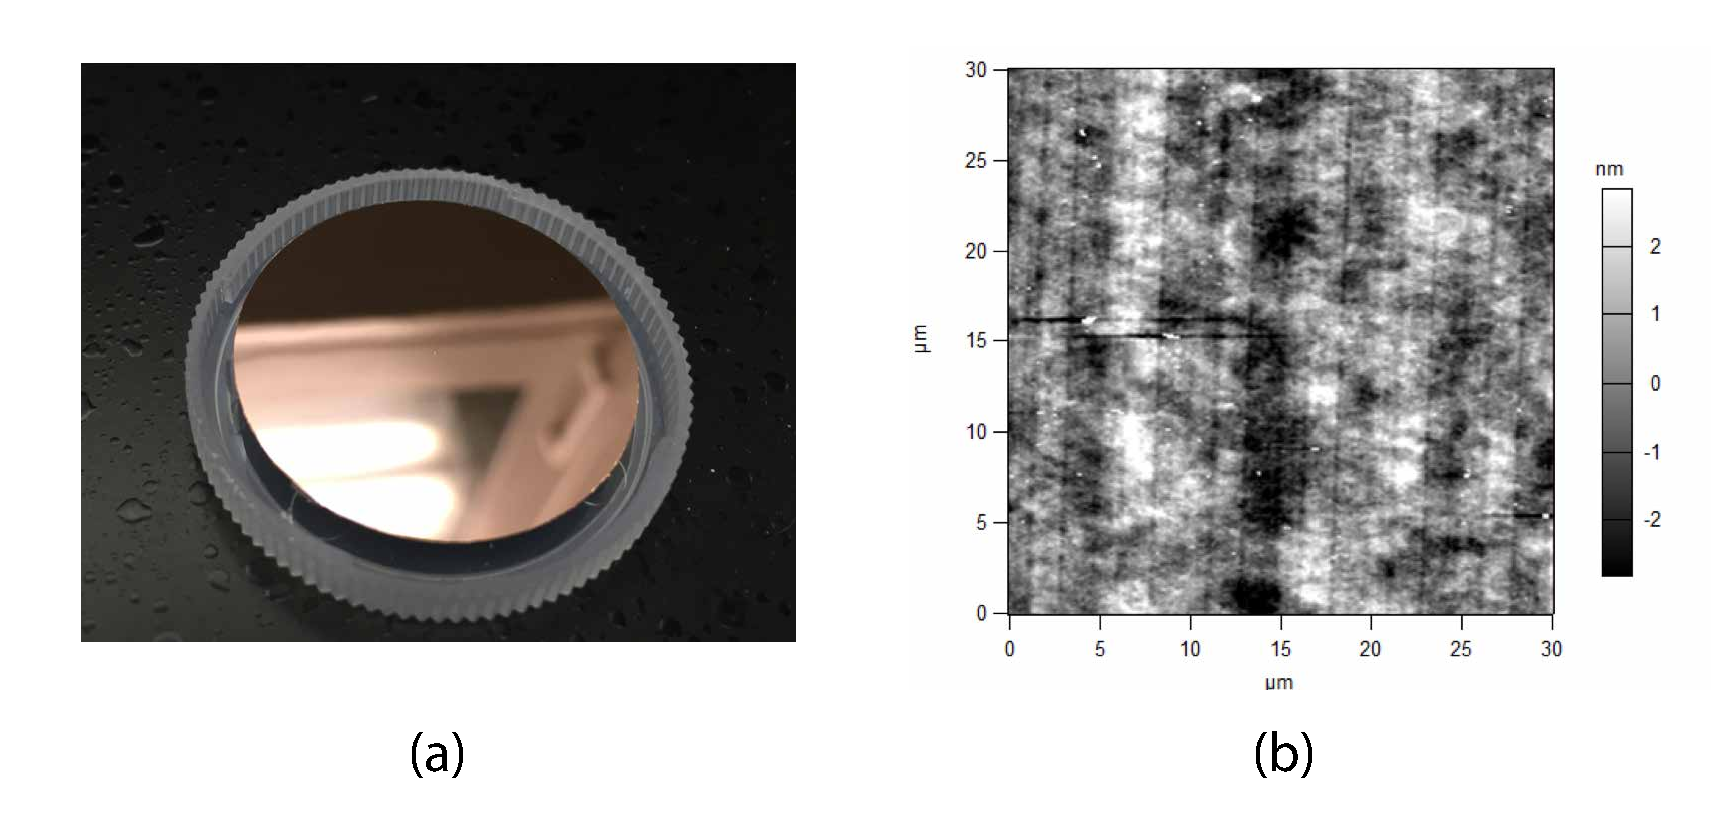
\includegraphics[width=1.0\textwidth]{Drawing/DTMCopper.pdf}
	\caption{(a) The copper foil after DTM thinning and polishing. The final thickness is about 100 $\mu$m. (b) The AFM image of the copper foil surface. The roughness is within 2 nm. Some nanoscale particles can be seen. They will serve as nucleation centers for graphene CVD growth. Reducing the density of surface contaminants will reduce the density of nucleation centers and enlarge the domain size. The vertical groves are left by the dents on the diamond tool for each revolution. The spacing between groves is the same as the approaching speed of the tool towards the center. The copper is annealed at $T = 1050^{\circ}$C for another time before growth starts and the surface will reconstruct, possibly remove those groves.}
	\label{FIG:DTMFinishing}
\end{figure}

Other than surface roughness, the copper domain size is another limiting factor for large single domain graphene growth. Although it was not clear the effect of copper substrate domains on the graphene quality\cite{kim2012direct, wang2012controllable, wofford2010graphene}, larger copper domain sizes gives us a chance to grow larger graphene single crystals. Annealing the copper at high temperature will reconstruct and merge the polycrystalline domains into larger domains, but mechanical processing will introduce defects and break the single domains, therefore the substrate needs to be re-annealed several times before graphene growth starts.

\begin{figure}[p]
	\centering
	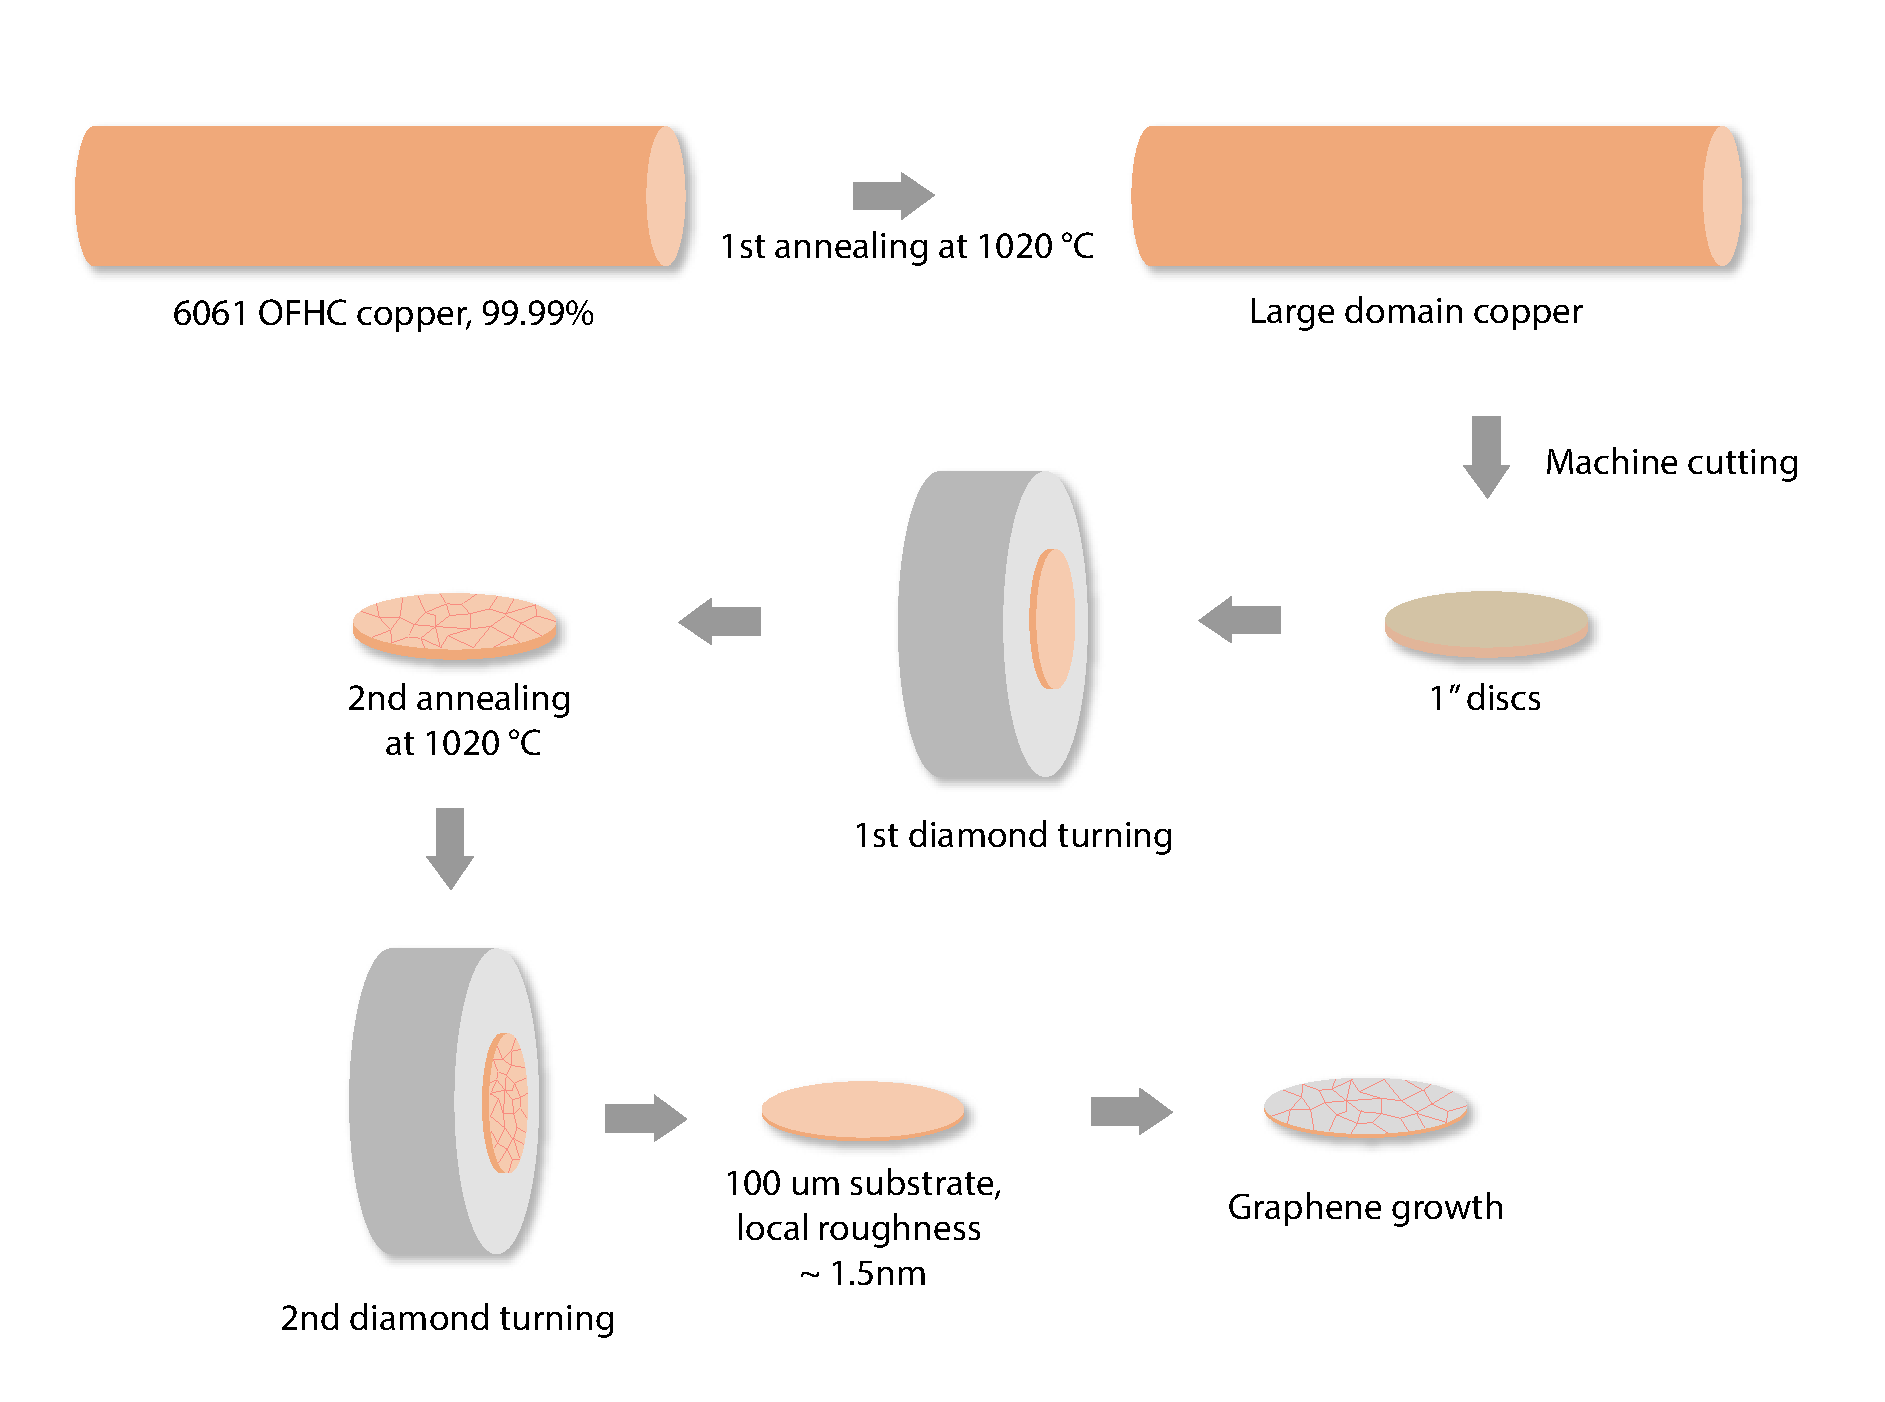
\includegraphics[width=1\textwidth]{Drawing/CopperProcessing.pdf}
	\caption{Procedure of cutting copper rods into 100$\mu$m foils for graphene growth. High purity OFHC copper rods are purchased from McMaster Carr. The rod is first annealed at 1050$^{\circ}$C for 24 h so that the polycrystalline domains merge into larger domains. Then the rod is cut into 2 mm thick copper discs in the machine shop. The discs are cleaned with DTM and then annealed again to ``heal'' the domains broken by the mechanical cutting. Domain re-formation would cause surface corrugation, therefore the copper disc surface is cleaned with DTM and then cut into 100 $\mu$m foils and ready for graphene CVD growth. }
	\label{FIG:CopperProcessing}
\end{figure}

The procedure of making copper rods into copper foils for graphene growth in shown in Figure \ref{FIG:CopperProcessing}. 1' long oxygen-free high thermal conductivity copper (OFHC) rods with ultra high purity (99.99\%) are purchased form McMaster Carr. The rod is first annealed at $T=1050^{\circ}$C for 24 h, and the polycrystalline domains will merge into larger domains within the rod. Then the rod is cut into copper discs of 2 mm thick in the machine shop. The mechanical cutting process will break the domains and introduce surface contaminant, so the surfaces copper discs are cleaned on the DTM, and then annealed again at 1050 $^{\circ}$C for 8 h. After annealing, the domain re-formation in the disc will cause corrugation on the surface. Therefore, the copper surface is cut with DTM for a second time. Then the copper discs are cut into 100 $\mu$m foils, by 10$\mu$m steps. During the thinning procedure, the copper will expand on the cutting face and cause deformation, and eventually break the vacuum sealing between the disc and spindle on the backside. Therefore the copper disc needs to be flipped several times to balance out the expansion and keep it flat when thinned from 2 mm to 100 $\mu$m. The process takes about 5 h. 

\subsubsection{CVD growth}

The CVD graphene growth can be performed in low pressure (LPCVD) or atmospheric pressure (APCVD). LPCVD grows graphene at a pressure lower than 100 mTorr, in continuous flow of pure hydrogen and methane and 1000 $^{\circ}$C substrate temperature. The problem with LPCVD is that the melting point of copper ($T_m = 1085^{\circ}$C) is close to the growth temperature. As a result, the copper will evaporate severely and contaminate the furnace\cite{vlassiouk2013large}. Also the pure precursor gases bring fire hazard. APCVD can eliminate those difficulties associated with the low pressure and improve the graphene quality\cite{vlassiouk2013large, dhingra2015quadratic}. Instead of using pure hydrogen and methane, APCVD uses gas mixture of 2.5 vol \% H$_2$, balance Ar and 0.1 vol \% CH$_4$, balance Ar. The furnace is pumped into low vacuum, and then backed-filled with hydrogen and methane mixture with argon to atmospheric pressure. The pressure from argon will suppress the evaporation of copper at annealing and growth temperature. The growth procedure are as follows\cite{dhingra2015quadratic}. 

\begin{itemize}
	\item The furnace is pumped down to $\sim$ 10 mTorr.
	\item Backfill the furnace with H$_2$/Ar mixture at 186 sccm, up to $\sim$ 100 Torr.
	\item Start the furnace temperature controller to ramp up to $T = 1050 ^{\circ}$C, and let the furnace stay at this temperature for 1 h.
	\item Start flowing mixture of CH$_4$/Ar at 14 sccm into the furnace, and let the copper foil stay in graphene CVD growth condition for 1.5 h.
	\item Cool down the system to room temperature. The flow of CH$_4$/Ar mixture is turned off at $\sim$ 650$^{\circ}$C. H$_2$/Ar mixture keeps flowing overnight until the system is below 50$^{\circ}$C. 
	
\end{itemize}

\begin{figure}[p]
	\centering
	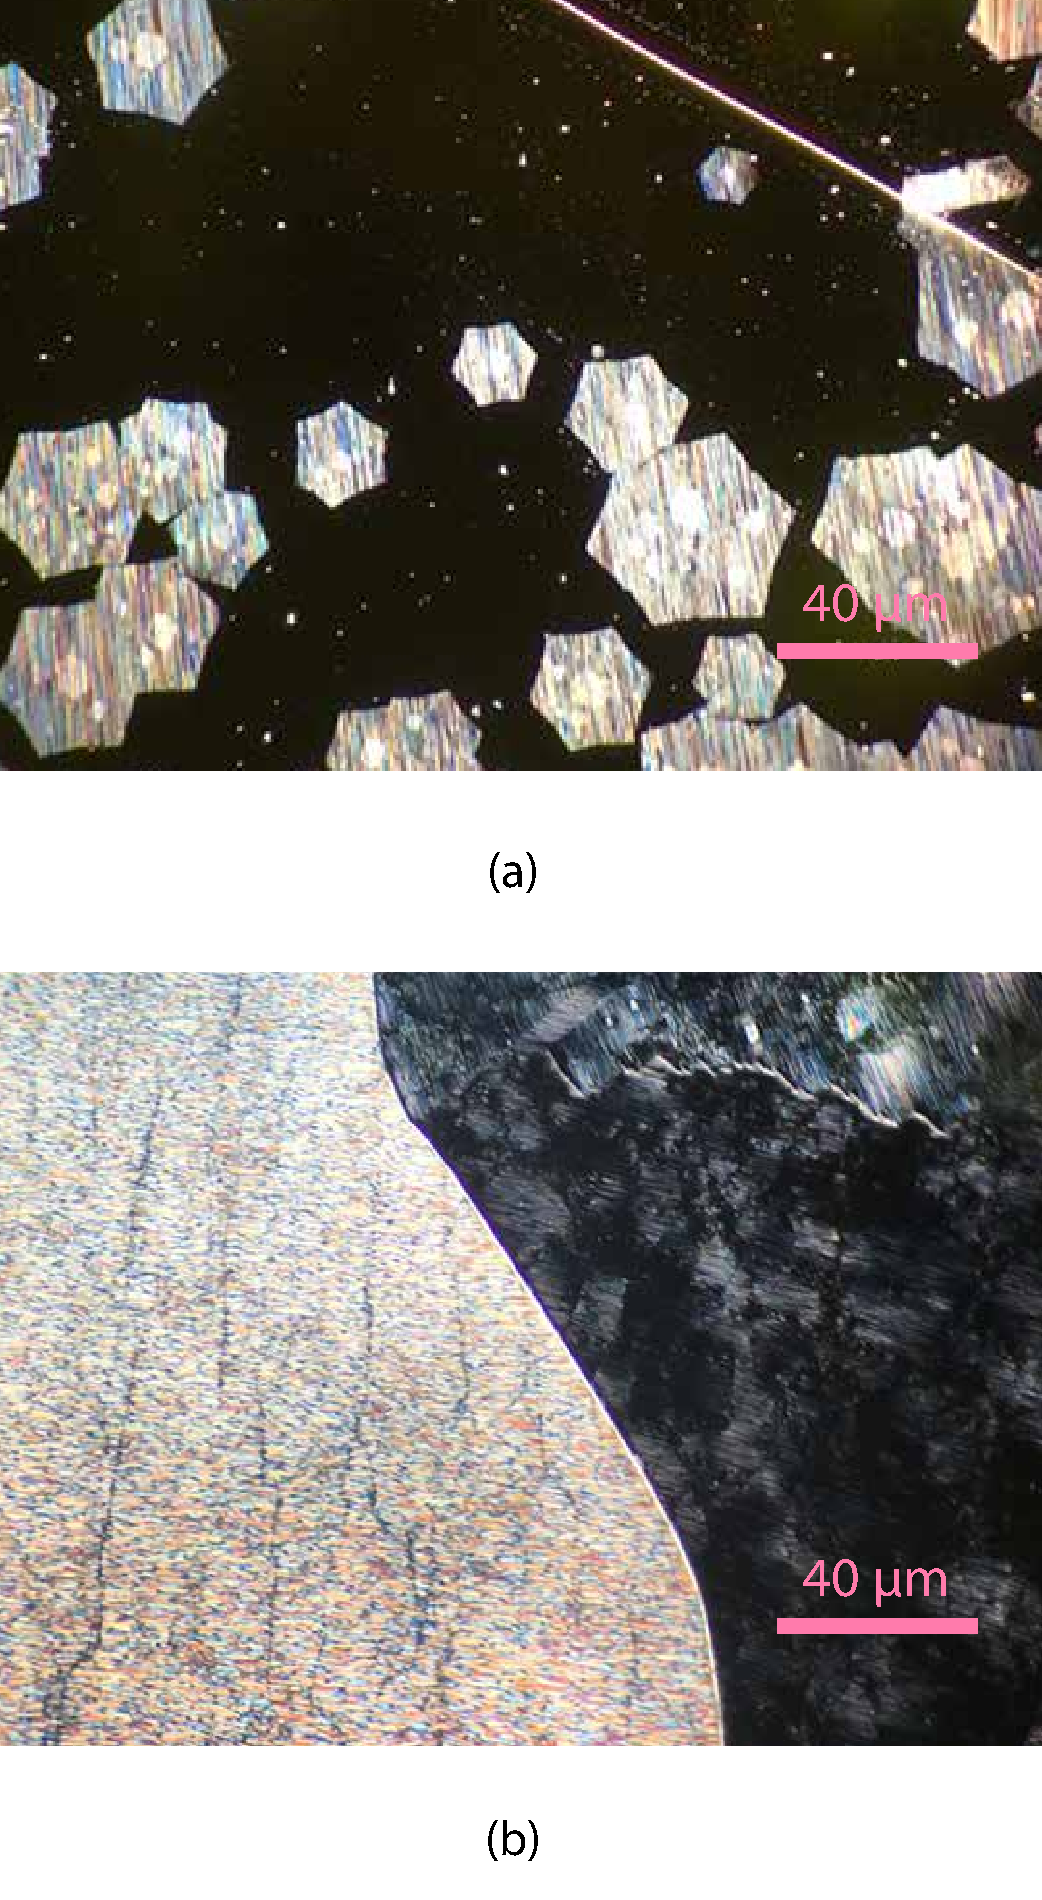
\includegraphics[width=0.6\textwidth]{Drawing/CVDGraphene.pdf}
	\caption{Dark field mode microscope images of CVD graphene on copper substrates. (a) The copper substrate is partially covered with graphene. Hexagonal shape single domain graphene can be observed. Growth was terminated before graphene fully covered the substrate. (b) Graphene covers the entire copper substrate. Copper domains of two different orientations can be observed. }
	\label{FIG:CVDGraphene}
\end{figure}

In Figure \ref{FIG:CVDGraphene} the dark-field mode of optical microscope clearly shows the CVD graphene on copper substrates. In \ref{FIG:CVDGraphene}(a) the copper substrate is partially covered with graphene. Growth process was terminated before graphene fully covered the substrate. Hexagonal shape of single domain graphene flakes can be identified. Some double layer can also be observed. On the top right corner of \ref{FIG:CVDGraphene}(a) a copper domain boundary can also be identified. \ref{FIG:CVDGraphene}(b) is the image of graphene grown in another run. The substrate is fully covered with graphene. The image shows two copper domains with different orientations, and therefore the graphene grown on the two domains look different. Wrinkles on graphene can be observed, resulting from different thermal expansion coefficient of copper and graphene. 

\section{LAO/STO sample processing}

One of the challenges with experiments on LAO/STO interface is to make good electrical contact from the bonding pads to the interface. A major part of my research is process the samples before the c-AFM writing can be performed, or graphene can be transferred. The processing methods have to be carefully chosen, so that the 2DEG and interface switchability will not be affected. Sample cleanness is another concern. Any nano-particles introduced in the processing would affect sample quality, considering that the dimensions of devices are also nanoscale. The procedure has those steps. Details of each steps can be found in the following subsections.

\begin{itemize}
	
	\item \textbf{Initial cleaning}: the sample is cleaned with acetone and isopropanol alcohol (IPA) in ultrasonic cleaner so that the particles introduced in shipping are cleaned. Usually I do not use deionized-water (DI-water) for cleaning. Proton from the water can get adsorbed on sample surface and affect the interface \cite{}.
	
	\item \textbf{Photolithography}: the sample is patterned with standard UV photolithography procedures, either with optical mask and UV lamp or with direct laser writer, for further processing. The finest features in my design are 2 $\mathrm{\mu}$m wide.
	
	\item \textbf{Ion milling}: after the desired patterns are developed on the photoresist, the sample is bombarded with Ar$^+$ ion flow so that the LAO/STO interface is exposed for electrical contact.
	
	\item \textbf{Deposition}: titanium and gold are used for making contact with the exposed LAO/STO interface either by electron-beam evaporation or sputtering.
	
	\item \textbf{Lift-off}: the excessive metal outside the patterns are removed by the lift-off process following the metal deposition. Like the initial cleaning process, I use IPA and acetone and do not use water as solvent.
	
	\item \textbf{Oxygen plasma cleaning}: the sample is covered with residue from liquid and photoresist, until it is cleaned with oxygen plasma cleaner. Then the atomic steps can be seen with AFM.
	
\end{itemize}
	
% The sample processing procedures are shown in FIG. \ref{}. 

% figure of processing

\subsection{Photolithography}
\label{SEC:Photolithography}

Photolithography is a commonly used technology in semiconductor industry. The substrate is covered with a thin layer of photosensitive material, and exposed under UV with designed pattern. UV would change the solubility of photoresist, and the pattern can be developed in buttered base solution after exposure. The modern state-of-the-art photolithography technology can reach resolution of 10 nm, and is the pillar of support for the semiconductor industry. There are two types of photoresists: positive and negative. Positive photoresist will be washed off after been exposed to UV, while negative photoresist is stabilized by UV and the unexposed parts are removed by developers. In my experiment, three types of positive photoresists are used: AZ4620, AZ4210 and AZ4110. For each sample, a 3'' carrier wafer is used as a fixture, because dimensions of the sample (5 mm $\times$ 5 mm $\times$ 1 mm) is non-standard and most photolithography instruments are designed for 3'' or 4'' wafer in the university facility. AZ4620 is used to fix the sample to the carrier wafer during spin-coating, exposure and other steps, as a cleanroom-safe ``epoxy''. 


\subsubsection{Spin-coating}

There are two limiting factors of the feature resolutions in photolithography: diffraction limit of light and photoresist thickness. Spin-coating is a standard technique to keep the photoresist thin and uniformly covering the sample surface. When the sample is spinning at a speed between 1000 rpm and 6000 rpm, the photoresist solution on sample surface would spread out. The liquid will be finally in equilibrium of viscosity, roughness of sample surface and centrifugation from spinning. After the spin-coating the sample is baked at a temperature around 100$^{\circ}$C to vaporize the remaining solvent in photoresist and stabilize the film before UV exposure. In my experiment, the spinning speed is 4000 rpm. Thickness of AZ4210 and AZ4110 are 2.1 $\mu$m and 1.1 $\mu$m, respectively. These two types of photoresists have the same chemical composition. They have different concentrations so they end up with different thickness at the same speed. Usually thinner films will have more stable performances for fine features (2 $\mu$m, to be specific). In the cases where photoresists are consumed in the processing, such as reactive ion etching, thicker photoresist will be a better option.

The spin-coating conditions are listed in Table \ref{tab:photoresistsCoating}.

\begin{table}
	\centering
	\begin{tabular}{l|cc}
		\hline
		Photoresist	&	AZ4210	&	AZ4110 \\ \hline
		Spinning speed	&	4000 rpm	& 4000 rpm	\\ 
		Spinning time	&	30 s	&	30 s	\\
		Baking temperature	&	95 $^{\circ}$C	&	95 $^{\circ}$C \\ 
		Baking time	&	60 s	&	60 s	\\
		Thickness	&	2.1 $\mu$m	&	1.1 $\mu$m \\ \hline
	\end{tabular}
	\caption{Spin-coating conditions for AZ4210 and AZ4110}
	\label{tab:photoresistsCoating}

\end{table}

% image of sample spin coated with photoresist. Explain the color stripes.

\subsubsection{UV exposure}

The UV exposure is to use short wavelength photon to change the solubility of photoresist, so that the following developing step can selectively remove the photoresist. Like all optical system, the resolution of exposure is limited by diffraction limit of light. Historically, mercury gas-discharge lamp is used, and 436 nm (``g-line''), 405 nm (``'h-line') and 365 nm (``i-line'') are selected as UV source. Besides Hg lamp, solid state laser and excimer laser with shorter wavelengths are also commonly used UV source. Samples are exposed with two different methods: mask exposure and direct laser writing. 

Mask exposure is performed by a mask aligner (Suss MJB3 or MA6, see Figure \ref{FIG:Suss}). Incoherent and collimated UV is generated from a Hg lamp and an area of 4'' $\times$ 4'' is exposed with UV at constant intensity of 10 mW/cm$^2$. The sample is covered with a photomask (Figure \ref{FIG:MASK}), a square piece of soda glass (to reduce UV absorption) coated with chromium on one side. The desired pattern is pre-printed on the chromium by chemical etching. The patterns on photoresist will be the copy of the patterns on the photomask. 

\begin{figure}[h!]
	\centering
	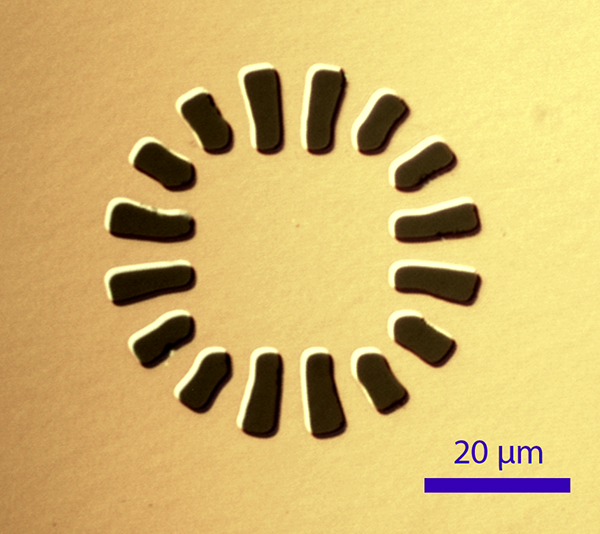
\includegraphics[width=0.5\textwidth]{Drawing/MASK.png}
	\caption{Mask for photolithography. The dark parts are transparant, while the bright parts are covered with chromium. Sample will be exposed where UV is not blocked by chromium. The figure shows the electrodes of a canvas for writing. The pedal shape area to be exposed will be etched away on the sample, and filled with titanium and gold to make contact with the LAO/STO interface.}
	\label{FIG:MASK}
\end{figure}

\begin{figure}[hp!]
	\centering
	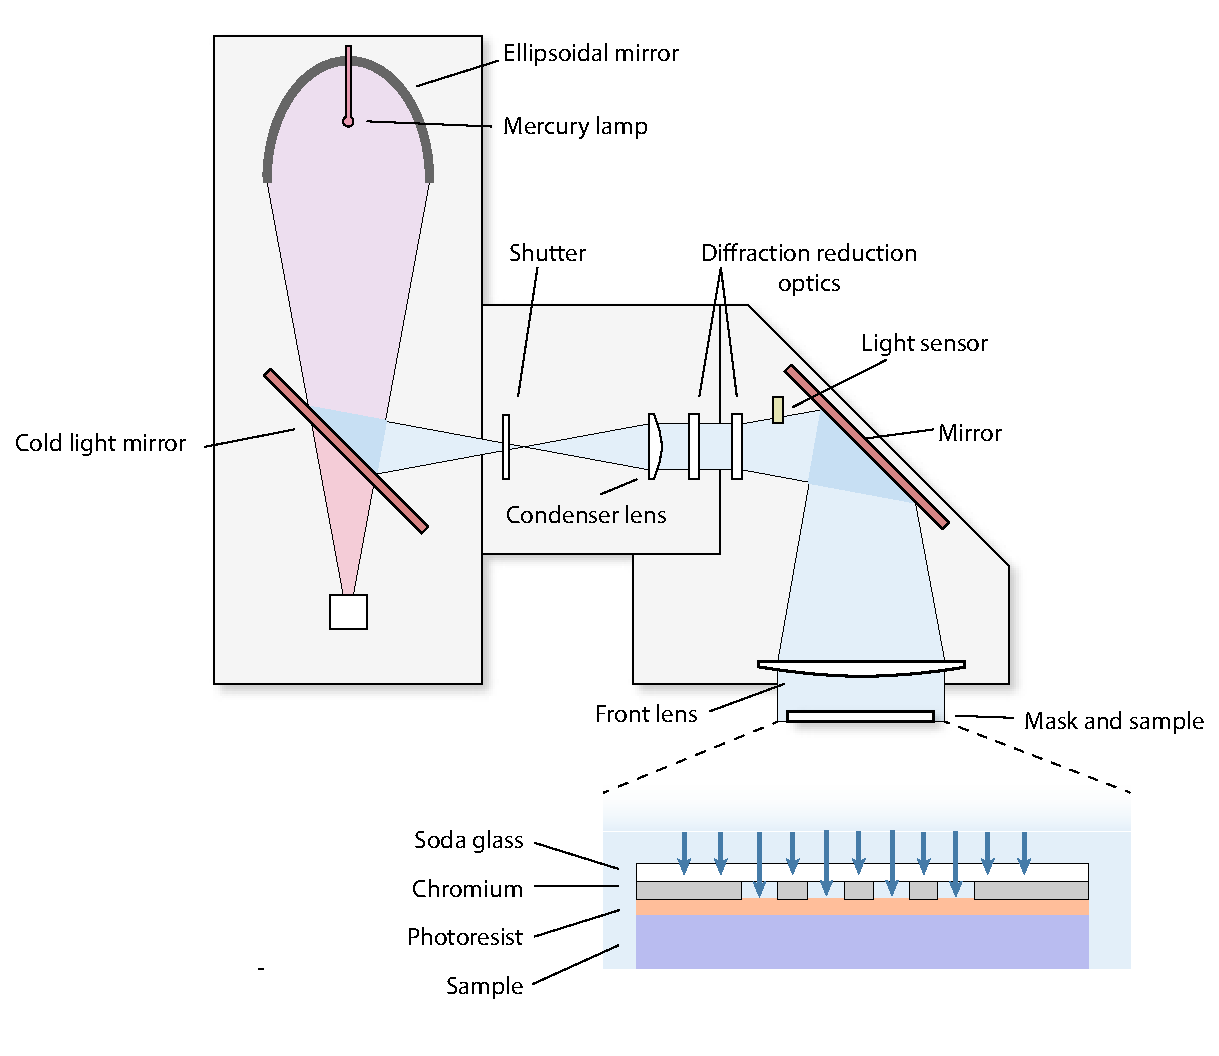
\includegraphics[width=1.0\textwidth]{Drawing/Suss.pdf}
	\caption{Suss UV mask aligner. The mercury lamp generates broad band light from arc. The light is reflected by an ellipsoidal mirror and focused on a cold light mirror, where the UV is selected. The exposure time and dose is controlled by a shutter. The UV is collected by a condenser lens and diffraction reduction optics for collimation and resolution enhancement. Finally, the UV is shed on the sample with a folding mirror and front lens. The sample is in close contact with a mask, where chromium is partially removed. UV exposes the photoresist on sample and print the mask pattern on it.}
	\label{FIG:Suss}
\end{figure}

Direct laser writing uses focused laser beam to write micro-patterns directly on photoresist, without using a mask. This is usually how the photomask is manufactured, but it can also be used to pattern samples. In my experiment I use Heidelberg MLA100 (Figure \ref{FIG:Heidelberg}), with 405 nm wavelength UV generated from a solid state laser. The laser is expanded and filtered with a pinhole, and focused on the sample with a high-NA objective. The focusing objective is fixed, and the sample is placed on a piezostage controlled with computer, to follow the designed pattern. The UV dose is determined by both the laser power and laser spot dwell time. It is important to keep the sample surface horizontal, so that laser spot will not defocus while moving through the entire sample surface. Sometimes, especially when the critical dimension is close to 2 $\mu$m, the photoresist patterns are not evenly developed, and it is caused by sample tilting and laser defocussing. Focusing quality can be checked with a real-time CCD image, while the sample is illuminated with red light from a second diode.

\begin{figure}[hp]
	\centering
	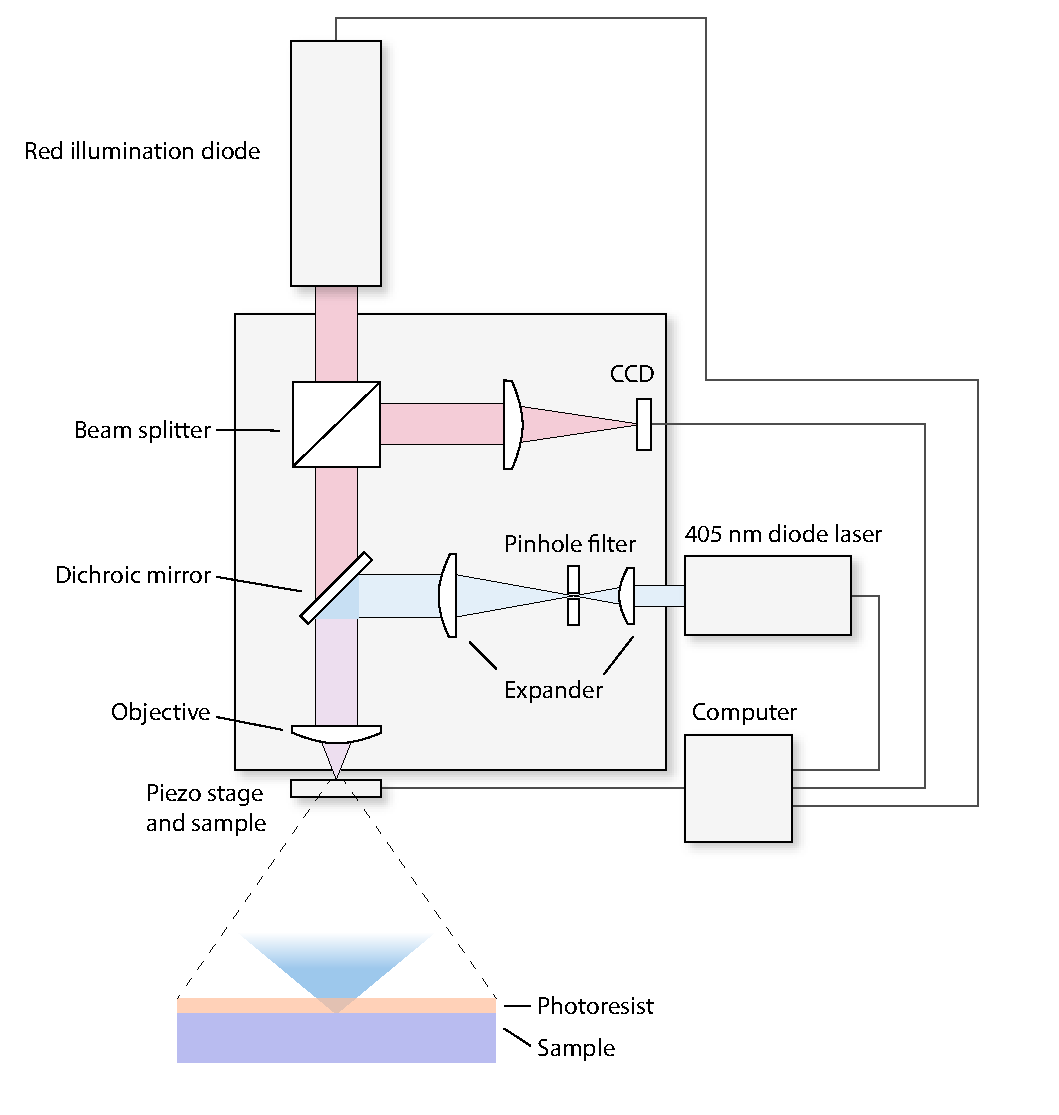
\includegraphics[width=1.0\textwidth]{Drawing/Heidelberg.pdf}
	\caption{Heidelberg direct laser writer. The sample is illuminated by red light from a diode, and realtime image of sample surface can be monitored with a CCD. UV with $\lambda=405$ nm is generated from a laser diode. The laser is expanded and filtered, and focused on the sample surface with a high-NA objective. The sample is fixed on a piezo-driven stage. The CCD image, laser power, sample movement and layer alignment are all controlled with computer, so that the laser path and dose control is fully automatic.}
	\label{FIG:Heidelberg}
\end{figure}

\subsubsection{Developing}

Developing is the process using buffered base solution to washed away the unwanted parts of photoresist after exposure and reveal the pattern on sample, for future processing steps. Depending on the type of photoresist, either the exposed parts (positive photoresist, such as AZ4210) or unexposed parts (negative photoresist, such as AZ5214) are removed. In my experiment I use AZ400K (potassium borate) for developing. The developer is diluted with DI-water, by 1:3 or 1:4 ratio. Different concentration will maintain different pH level and developing speed. The sample is washed with DI-water after developing, to remove the excessive developer. 

A picture of sample after UV exposure and developing is shown in Figure \ref{FIG:Developed}. Photoresist in the bright area are washed away while the rest of the sample is still covered with photoresist. Note that the edges of the pattern are less sharp than the mask, because of the resolution limit from diffraction. 
\\
\begin{figure}[h!]
	\centering
	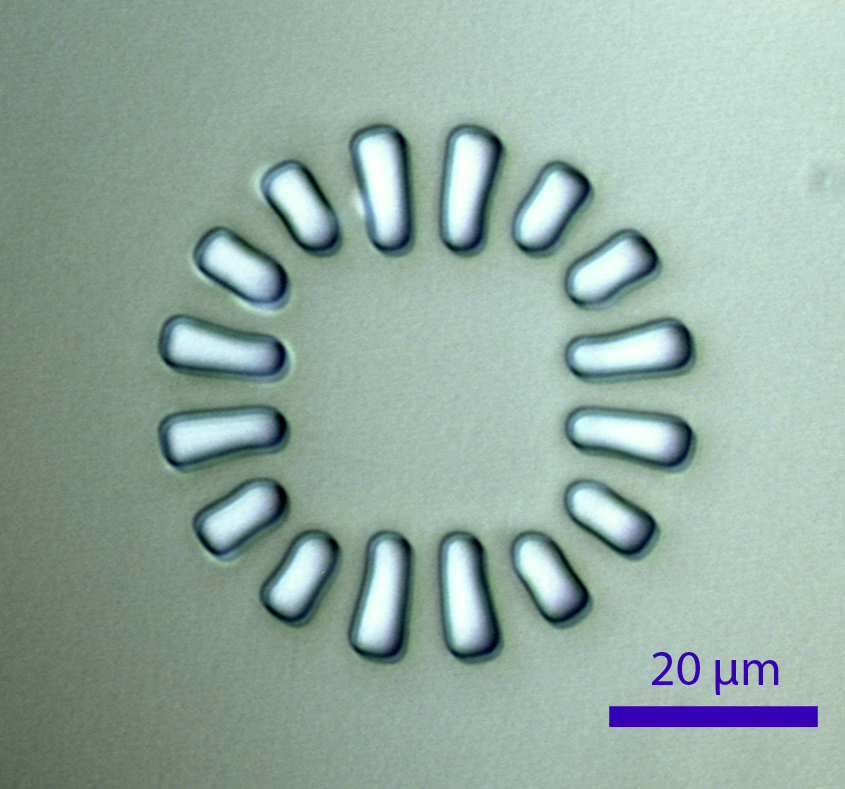
\includegraphics[width=0.5\textwidth]{Drawing/Developed.png}
	\caption{Exposed and developed sample. The bright regions are free of photoresist while the rest of the sample is still covered.}
	\label{FIG:Developed}
\end{figure}

The conditions for exposure and developing are listed in Table \ref{tab:photoresistsExposureDeveloping}.

\begin{table}[h!]
	\centering
	\begin{tabular}{l|cc}
		\hline
		Photoresist	&	AZ4210	&	AZ4110 \\ \hline
		UV Dose	&	170 m$J$	& 100 - 120 m$J$	\\ 
		Developer : Water	&	1 : 4	&	1 : 4	\\
		Developing time	&	120 - 180 s	&	120 - 180 s \\ 
		Resolution	&	3 - 5 $\mu$m	&	2 $\mu$m	\\ \hline
	\end{tabular}
	\caption{UV exposure and developing conditions for AZ4210 and AZ4110}
	\label{tab:photoresistsExposureDeveloping}	
\end{table}

 Photolithography is the part that has the most uncertainty in the entire processing, and can affect some samples (like graphene/LAO/STO) more significantly. This will be discussed in future sections. 

\subsection{Ion milling}
\label{SEC:IonMilling}
LAO/STO interface is buried underneath LAO, so if contact need to make with the interface the LAO has to be etched. Usually there are three methods for etching: wet chemical etching, dry plasma etching and ion milling. Wet chemical etching using reactive chemical solutions (such as HF, HCl) to etch away the materials. This is  cheaper but less controlled, and etching is isotropic. Plasma etching, uses the plasma or free radicals of active gas molecules (such as O$_2$, SF$_6$, etc) to react and remove materials, at pressure between 0.1 and 5 Torr. It is better controlled in etching rate and directionality, but the instrument is more expensive, and finding the right gas to selectively etch the target material while keeping the protecting layer intact is not always feasible. Although there are mature industrial solutions for silicon, alumina and silica etching with plasma, there is not a good solution to etch complex oxides like LAO/STO with our facility plasma etcher. Ion mill uses accelerated ionized argon plasma to physically bombard sample. The etching rate is slower than the previous two methods, but performs well on most inorganic materials including LAO/STO. Also, the etching is more directional. In Table \ref{tab:etching} is a comparison of the three etching methods.

\begin{table}
	\centering
	\begin{tabular}{l|ccc}
		\hline
		Method	&	Chemical etching	&	Plasma etching	& Ion milling \\ \hline
		Cost	&	low	& high	& high \\ 
		Directionality	&	anisotropic	&	anisotropic	&	isotropic \\ 
		Selectivity	&	high	&	high	&	low \\
		Speed control	&	poor	&	good	&	good \\
		Target material	&	inorganic	&	organic or inorganic	&	inorganic \\
		Environment	&	aqueous, ambient	&	0.1 - 5 Torr, vacuum	&	$< 10^{-4}$ Torr, vacuum \\
		\hline  
		
	\end{tabular}
	\caption{Comparison of etching methods.}
	\label{tab:etching}
	
\end{table}

Ion mill accelerates Ar ions to a certain kinetic energy and physically etch samples with bombardment. As shown in Figure \ref{FIG:IonMill}, Ar$^+$ is generated from the discharge chamber. The entire chamber is pumped to high vacuum ($< 10^{-6}$ Torr), and back filled with Ar gas to $10^-4$ Torr. On the right-hand-side of the figure, a filament is heated up and a biased voltage is applied between the filament and chamber wall. Electrons are extracted from the filament and ionize the argon molecules. Usually a magnetic field is applied through a solenoid to increase the path and ion yield before the electrons reach the chamber wall. At the opening side of the discharge chamber, there are two or three layers of electrically isolated screen grids (made of sputter-resisting materials like Mo or W). A voltage of 500eV is applied between the grids so that Ar$^+$ can be accelerated to the same energy. The pores on the grids are aligned so that the Ar$^{+}$ flow is collimated. Right after the Ar$^{+}$ exits the chamber, it is mixed with free electrons from a neutralizer filament, so that flow will not be diverged by coulomb attraction between Ar$^{+}$ before they reach the sample. The sample is 20$^{\circ}$ to 30$^{\circ}$ off the normal direction, to create undercut and facilitate electrical contact between the interface and the electrodes. The kinetic energy of the plasma is converted to heat on the sample surface. Either the sample is cooled down with flowing water inside the chuck, or the plasma flow is shutoff with a duty cycle so that the sample can cool down by radiation. Temperature over 150 $^{\circ}$C will cause phase transition of the photoresist on the sample, and make hard to remove by lift-off.

\begin{figure}[hp]
	\centering
	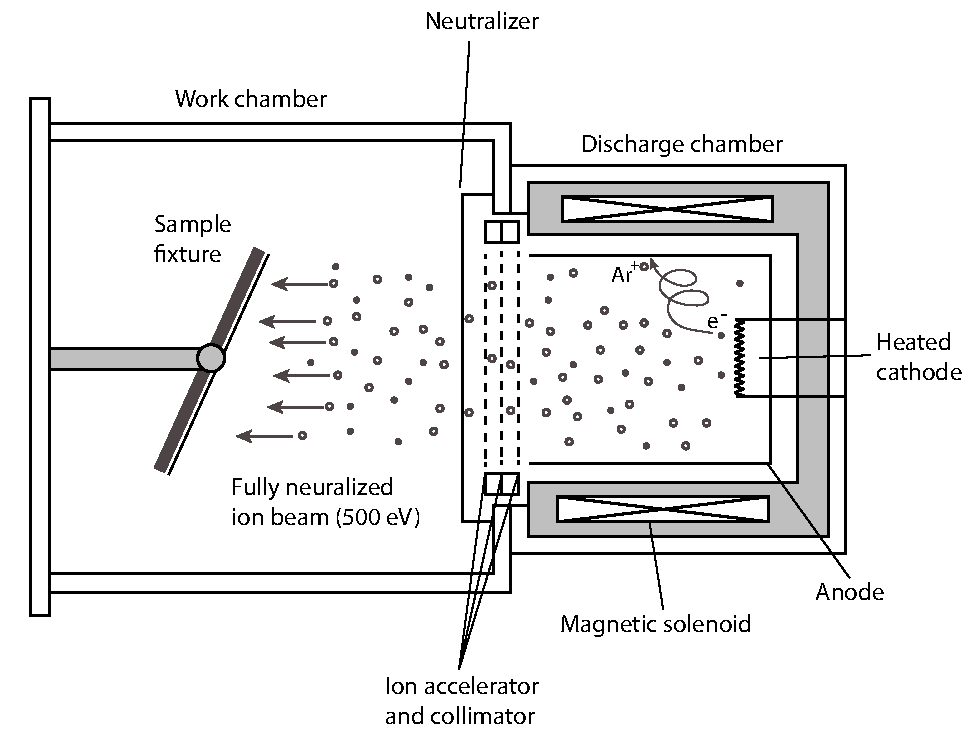
\includegraphics[width=1.0\textwidth]{Drawing/IonMill.pdf}
	\caption{Simplified view of ion mill. The argon ions are generated from the discharge chamber on the right hand side. Electrons are extracted from the heated cathode and ionize Ar molecules before they reach the chamber, which works as an anode cup. A magnetic field is applied through a solenoid to increase electrons' path. Ar$^{+}$ are accelerated and aligned by the grids to 500 eV. Electrons from the neutralizer are mixed with the Ar$^{+}$ plasma flow so that the collimation can be maintained. Sample is tiled by an angle of 22.5$^{\circ}$.}
	\label{FIG:IonMill}
\end{figure}

\subsection{Deposition}

Titanium and gold are used for making contact with the interface of LAO/STO. I use two methods to deposit the material: sputtering and electron-beam (e-beam) evaporation. Sputtering is similar to ion milling, but instead of using Ar$^{+}$ plasma flow to bombard and etch the sample, it is directed towards the target materials (Ti, Au, etc). The binding energy of the target material atoms is much smaller than the kinetic energy of Ar$^{+}$, and are ejected from the target and deposit onto the sample surface. E-beam evaporation (Figure \ref{FIG:Ebeam})controls electron-beam to heat up the target material and vaporize it. The vapor is thrown through a long distance ($> 10$ cm) before it reaches the sample. Compared to sputtering, the e-beam evaporation is more directional, because of the long throw-distance of evaporated material, compared to sputtering. 

As can be seen in Figure \ref{FIG:Ebeam}, a beam of electron is accelerated by a high voltage of 10 kV. The direction and shape of the beam is controlled by magnetic field. The material is loaded in a crucible and heated up by the e-beam, and evaporated. The material is thrown upward, towards the loading chamber where the sample is located. A shutter is used to control the deposition time of material. Deposition rate is controlled by the e-beam current. The sample can be tilted if needed, to improve the electrical contact to the interface.

The pressure of the chamber is maintained at $< 10^{-6}$ Torr to avoid any oxidation of material during deposition. Also, when titanium is used to make contact between gold bonding pads and LAO/STO interface, a pre-deposition evaporation of 10 minutes is required. The evaporated titanium can trap the remaining oxygen molecules in the chamber, and further reduce the oxidation on the target metals. 

\begin{figure}[p]
	\centering
	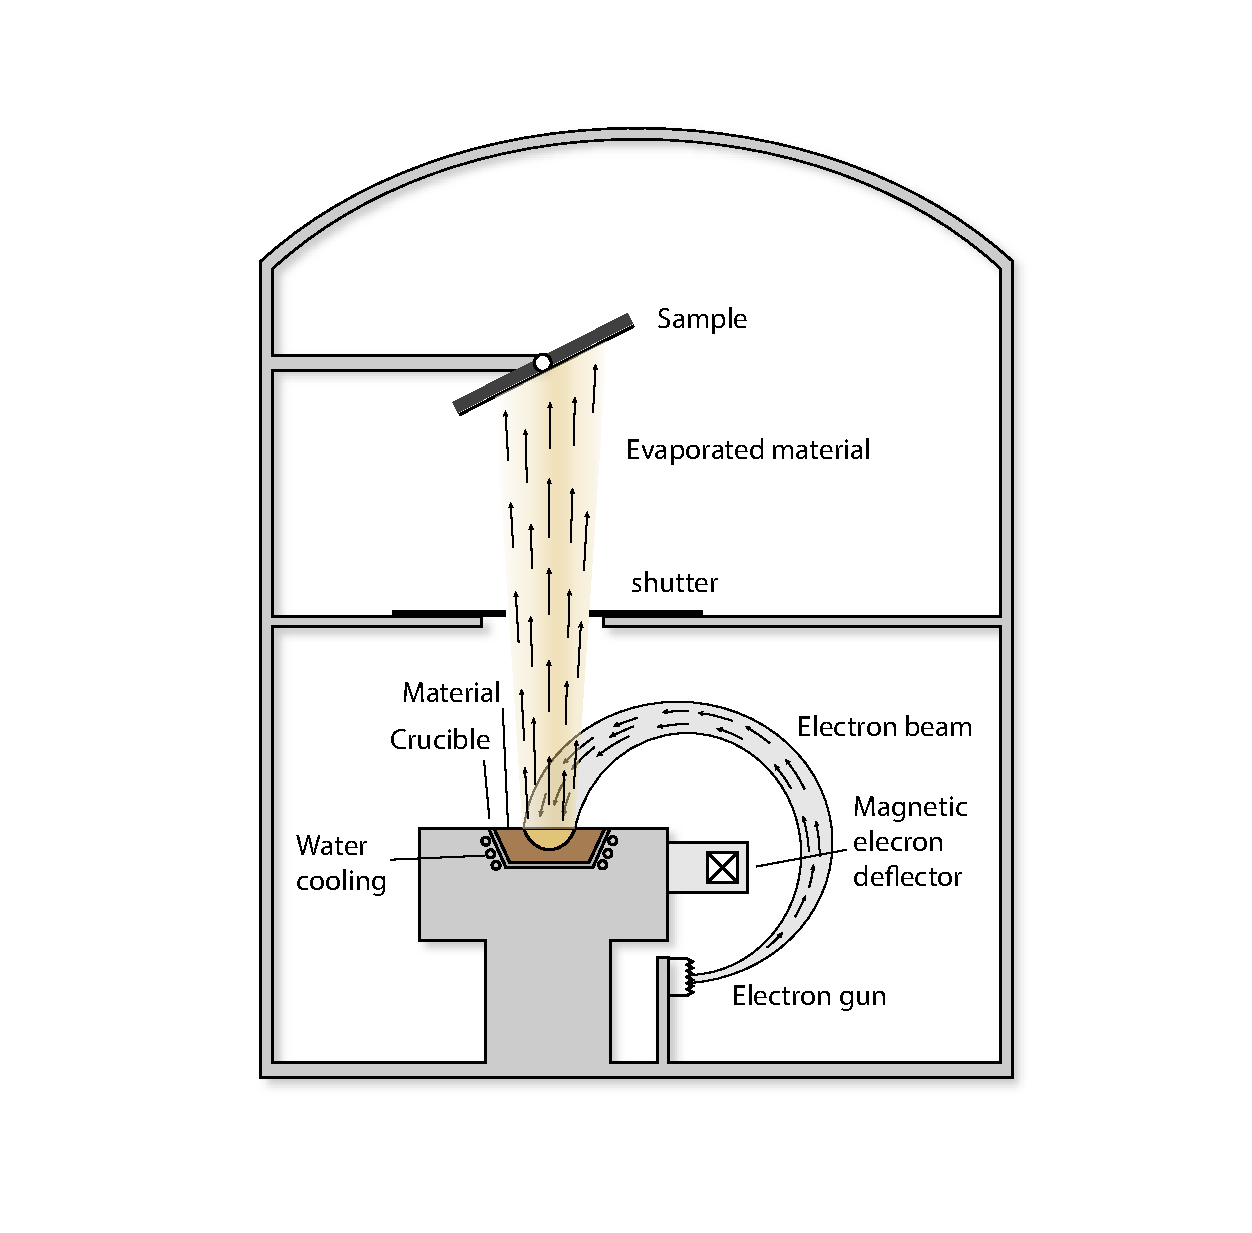
\includegraphics[width=1.0\textwidth]{Drawing/Ebeam.pdf}
	\caption{E-beam evaporator. The electron beam is generated from an electron gun on the bottom. The beam is deviated and shaped by magnetic field, towards the material. Them material is loaded in a crucible and heated up to melting point. The vapor of the material is thrown towards the sample on top. Deposition time is controlled by a shutter.}
	\label{FIG:Ebeam}
\end{figure}

\subsection{Lift-off}

When the sample is patterned with photolithography and coated with metal, the photoresist and the excessive metal need to be removed. Photoresist can dissolve in organic solvents such as acetone. Acetone has high vapor pressure, so it is not suitable to be heated up to increase solubility of photoresist. Also, when acetone dries up on sample it forms streaks. Therefore the sample needs washed with IPA to remove the acetone residue. When the photoresist is heated up to 140 $^{\circ}$C, it will cross-link and its solubility in will decrease. 1165 remover (1-methyl-2-pyrrolidone, or NMP) need to be used for lift-off in such cases. It has low vapor pressure and can be heated up to 80 $^{\circ}$C. If 1165 still cannot fully remove the photoresist after sample is immersed in it for 24 hours, oxygen plasma cleaner is needed.

\subsection{Oxygen plasma cleaning}

The oxygen plasma cleaner activates oxygen molecules with a high frequency voltage (kHz to MHz) in low pressure, and forms plasma or oxygen radicals when electrons recombine with oxygen ions. The mixture is highly reactive and interactive with organic materials like photoresist residue on sample surface. Oxygen plasma cleaning can be categorized as a form of RIE (as discussed in Section \ref{SEC:IonMilling}), but it usually operates at high end of 100 mTorr and the etching is less directional. Compared to chemical solvent, oxygen plasma removes the photoresist residue at a much lower speed (about 10 nm/min), but the finishing is much cleaner, while less invasive compared to RIE. Therefore, oxygen plasma is used as a final step for sample processing.


\section{Atomic force microscope}
\label{SEC:AFM}

The atomic force microscope (AFM) is a type of of instrument that uses a nanoscale probe to interact with the surface, and characterize the properties (topography, coulomb interaction, conductivity, etc) of a sample. It was invented in IBM lab by Bin, Quate and Gerber \cite{} in 1986 and later commercialized in 1989. The development of AFM technology benefited from the advancement of STM and precise closed-loop spatial control using piezoelectric effect. However, AFM was invented to overcome the drawback of STM --- only conductive or semi-conductive samples can be measured. AFM can measure various types of interaction between the probe and surface, such as surface potential, magnetic force, Van de Waals force, etc. Also, unlike the scanning electron microscopy (SEM) or tunneling electron microscopy (TEM), the AFM can be operated in various environment (aqueous, ambient, vacuum or cryogenic), and does not require the sample to be pre-treated (such as metal coating) or being conductive. The robustness and non-invasive nature of AFM make it a powerful tool for studying surface phenomena including charge density, magnetic dipole moment, capacitance, chemical bonding, nano-device lithography, and even biomacromolecules. AFM can also be integrated with other techniques, such as infrared spectroscopy\cite{}. The limitation of AFM is that the imaging cannot be as fast as SEM or TEM, as it relies on the physical movement of the tip.

\subsection{Working principle}


The AFM is mainly consist of three parts, as shown in Figure \ref{FIG:AFM}, AFM tip, laser optics, and piezoelectric scanning system. The AFM tip has a sharp end, with a radius of curvature in nanometer scale. A laser is reflected from the top surface the AFM tip and collected by a quad detector. The quad detector determines the position by
\begin{equation}
\begin{split}
I_\mathrm{sum} & = I_A + I_B + I_C + I_D \\ 
I_\mathrm{vdiff} & = (I_A + I_B) - (I_C + I_D) \\ 
I_\mathrm{hdiff} & = (I_A + I_C) - (I_B + I_D),
\end{split}
\end{equation}
where $I_A$, $I_B$, $I_C$ and $I_D$ are the intensities on the four quadrants of the detector. $I_\mathrm{sum}$ is the total intensity. $I_\mathrm{hdiff}$ and $I_\mathrm{vdiff}$ are the horizontal difference and vertical intensity difference. Assume the laser spot has Gaussian distribution. When the center of laser spot changes, the distribution of intensity on the four quadrant would change. The detector can monitor the movement by the horizontal and vertical differences in intensities. 

\begin{figure}[h!]
	\centering
	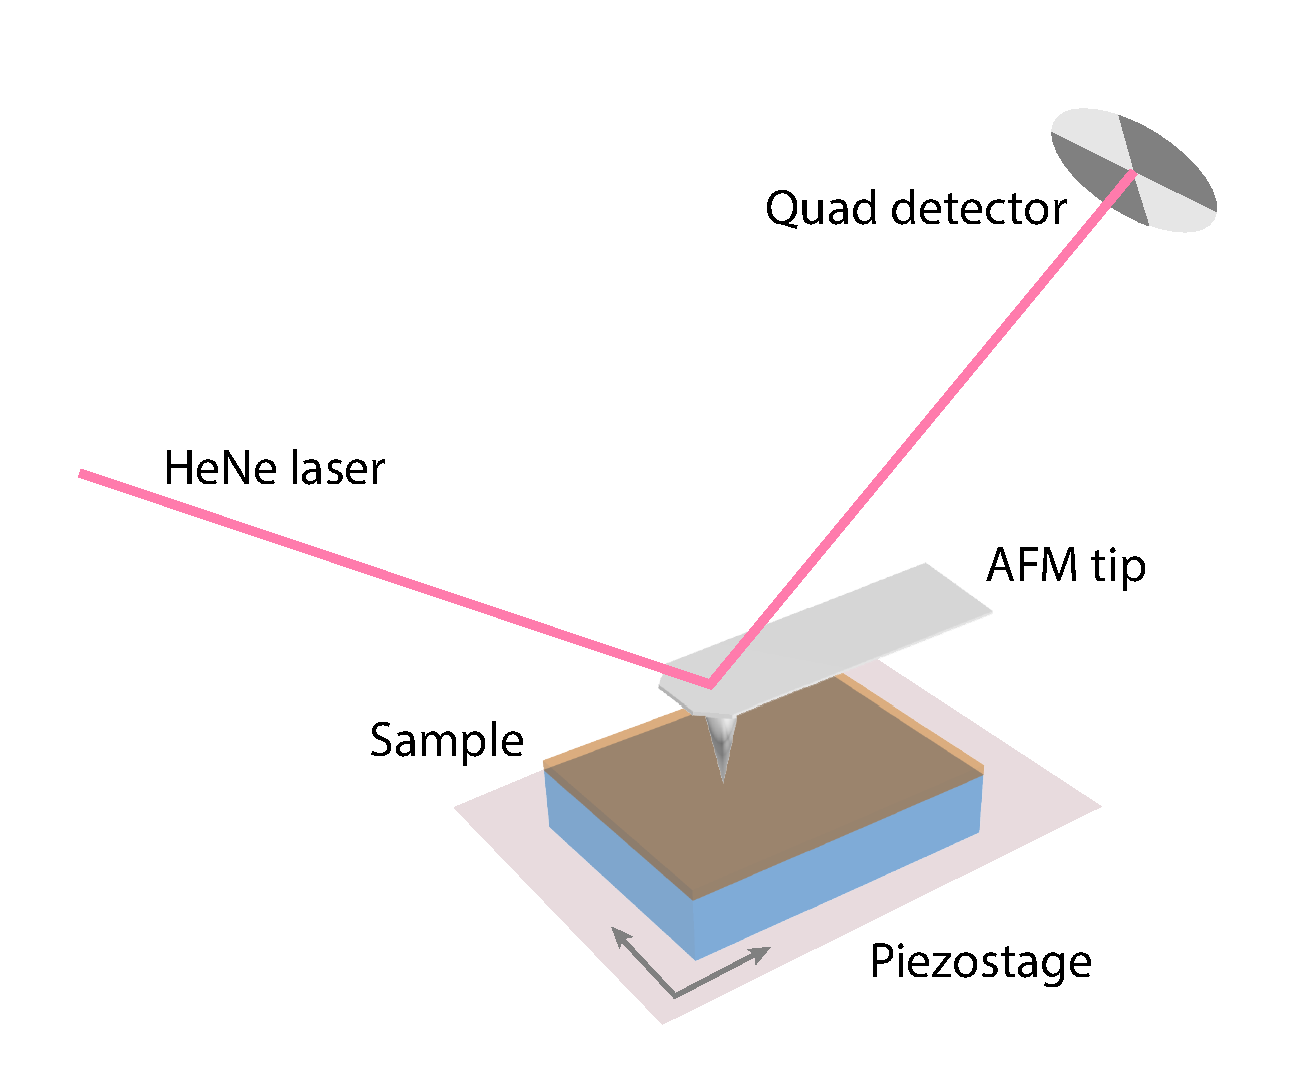
\includegraphics[width=0.8\textwidth]{Drawing/AFM.pdf}
	\caption{The schematics of AFM. A laser is reflected from the top surface of the AFM tip, and collected by a quad detector. A small amount of deformation would cause the center of laser spot to move on the quad detector, and measured as a change of differential voltage.}
	\label{FIG:AFM}
\end{figure}

When the interaction between the tip and sample surface changes and the tip is is slightly deformed, the laser spot would move on the quad detector. The deformation of tip follows Hooke's law:
$$F = -k \cdot x$$
Where $x$ is the amount deformation, and $k$ is the spring constant of the tip cantilever. $k$ is mostly between 1 N/m and 100 N/m, depends on the type of the tip. In my experiment I use tips with spring constant $k = 3$ N/m. The interaction between the AFM tip and sample surface is a function of distance. The attractive interaction decays slower than the repulsive interaction, therefore the total interaction follows the curve in Figure \ref{FIG:Interaction}.

\begin{figure}[h!]
	\centering
	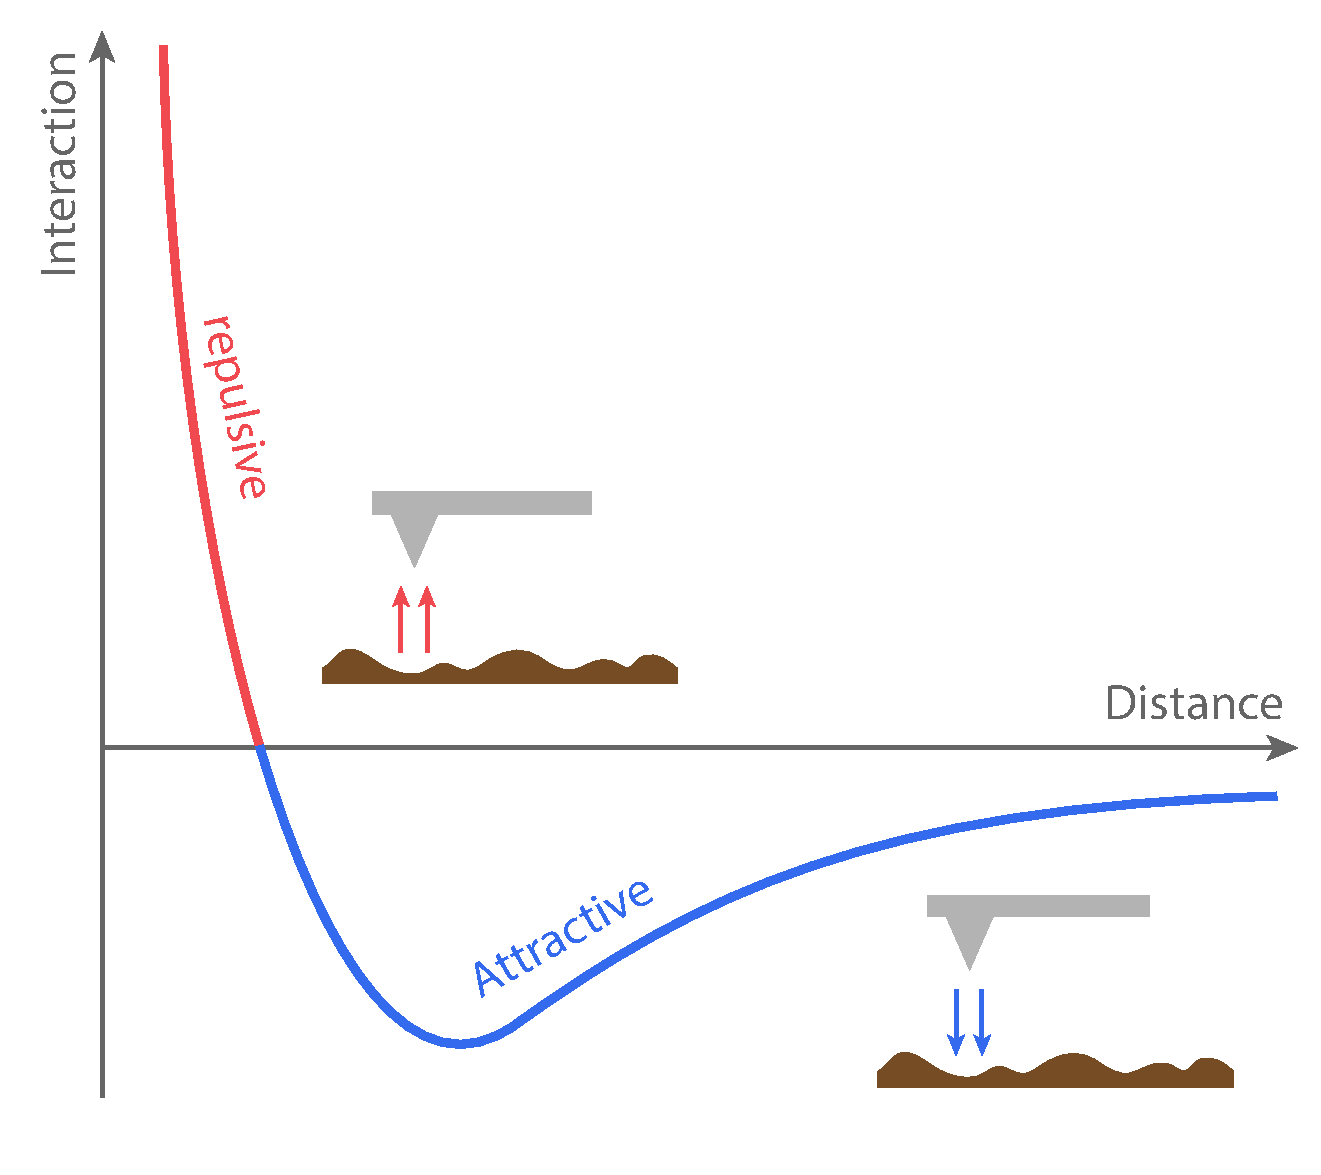
\includegraphics[width=0.7\textwidth]{Drawing/Interaction.pdf}
	\caption{The interaction between tip and the sample surface. At long distance the interaction zero. When the tip moves towards the sample, the interaction is attractive. As the tip gets closer, the interaction would switch from attraction to repulsion, and gets larger and larger the tip moves closer.}
	\label{FIG:Interaction}
\end{figure}

The sample is located on the piezoelectric scanning stage. The movement of the sample and the tip, and signal from the laser optics system are controlled and monitored by a computer. The type of signal depends on the working mode of AFM and nature of the interaction it is targeting. More details are discussed in the following sections. 

\subsection{Contact mode}

In contact mode, the AFM tip is in close contact with the sample. The distance between the tip and sample is controlled by a piezoelectric actuator. As shown in Figure \ref{FIG:ContactAFM}, When the tip approaches the sample surface, repulsion from the sample would deforms the tip and changes the reflection angle of laser spot. The intensity difference on the quad detector would also change, in terms of a voltage signal. When the sample is driven by the piezostage and cause the tip moves relative to the sample, the repulsive force between the tip and sample surface is regulated by a feedback loop between voltage on the piezoelectric actuator, and the voltage difference on the quad detector, so that the amount of tip deformation and repulsive force is a constant. 

\begin{figure}[h!]
	\centering
	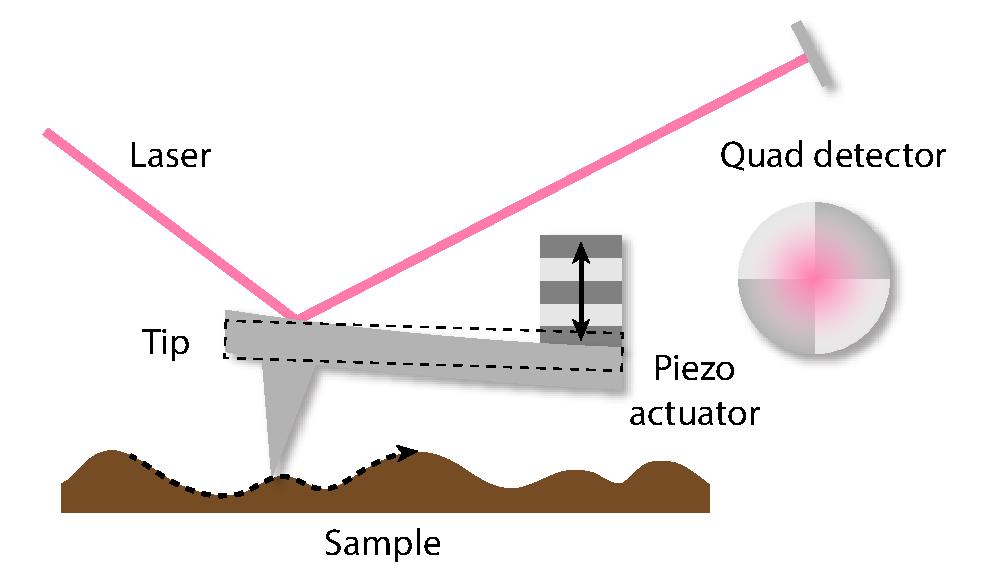
\includegraphics[width=0.6\textwidth]{Drawing/ContactAFM.pdf}
	\caption{AFM contact mode. The tip is pressed to the sample surface by the piezoelectric actuator. The deformation of the tip is monitored by the quad detector. The voltage of the piezoelectric actuator is controlled with a feedback loop with the deflection voltage on the quad detector.}
	\label{FIG:ContactAFM}
\end{figure}


\subsection{AC mode}

In AC mode, the AFM tip is driven by a sinusoidal electrical signal on the tip piezoelectric actuator, as shown in Figure \ref{FIG:ACAFM}. The electric frequency is close to the resonance frequency of the tip (10 kHz - 500 kHz). The driving frequency is not exactly at the resonance frequency, so that the gradient of amplitude change is maximized and the system is most sensitive to the interaction change. The laser spot and difference signal also oscillates at the same frequency. When the tip approaches the sample surface, the interaction between the tip and surface will cause the resonance frequency to shift and change the amplitude $A$ and phase $\theta$ of the tip oscillation and monitored by the differential voltage signal on the quad detector. The measurement can be integrated with lock-in amplifier technique for noise reduction. When the tip scan through the surface, $A$ and $\theta$ are recorded for each position on the sample surface and mapped onto a 2D image. The voltage on the piezoelectric actuator ($z$ voltage) is controlled by a feedback loop so that the amplitude $A$ is maintained at a set point. During the scan the tip is not continuously in contact with the sample surface, but ``tapping'' the sample with oscillations, therefore AC mode is sometimes called ``tapping mode''. Compared to contact mode, in the AC mode the tip does not scratch the sample surface, so it has less effect on the sample. 

\begin{figure}[h!]
	\centering
	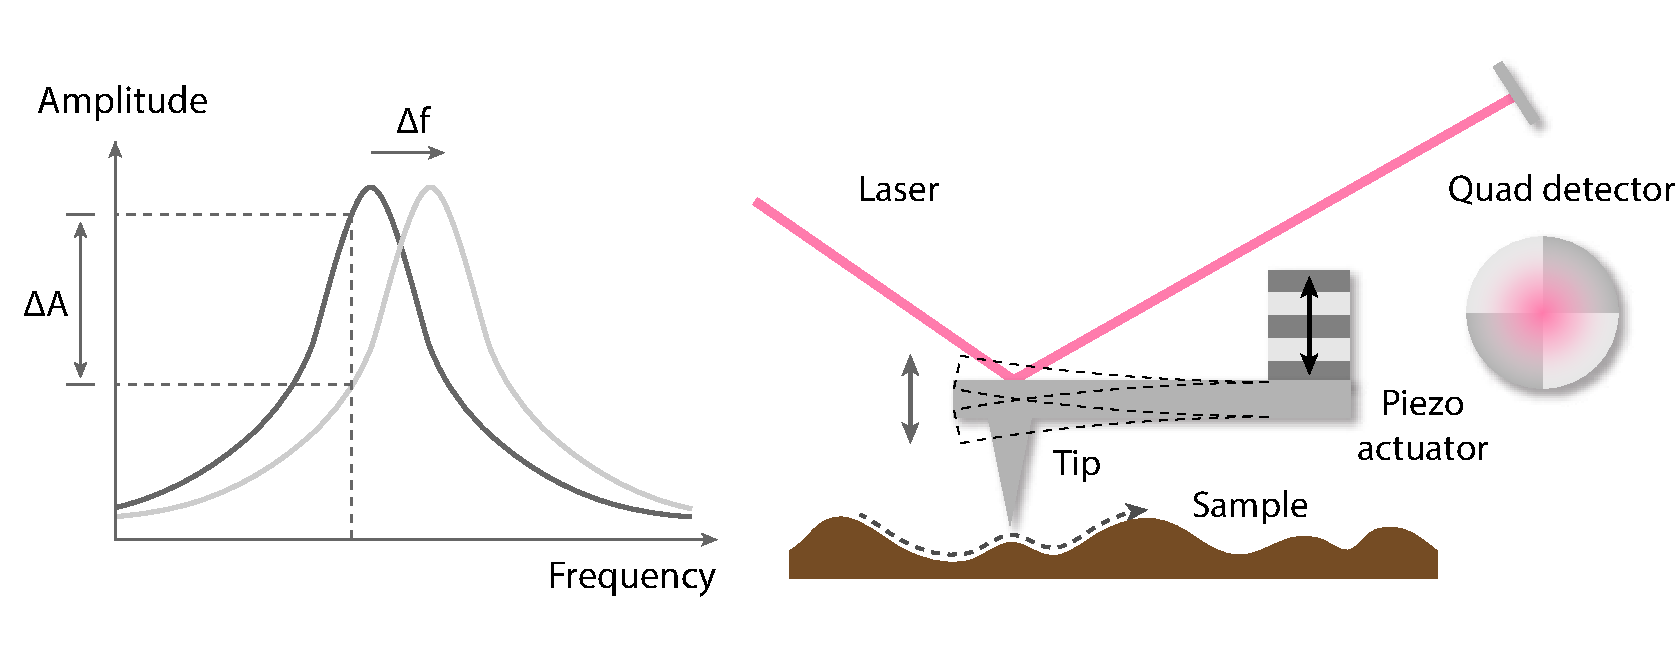
\includegraphics[width=1.0\textwidth]{Drawing/ACAFM.pdf}
	\caption{AFM AC mode. Left: the tip is driven at a frequency close to the resonance frequency. When the resonance frequency shifts as the interaction between the tip and the sample changes, the Change of oscillation amplitude is monitored by the quad detector and sent to the computer.}
	\label{FIG:ACAFM}
\end{figure}

\subsection{Non-contact mode}

In the non-contact mode, the tip is maintained at the attractive regime so that the sample does not have direct contact with the tip. The tip and the sample is maintained at distance that the interaction is always attractive while the tip is scanning through the sample (Figure \ref{FIG:NonContactAFM}). This is especially important for biomacromolecules and organism. 

\begin{figure}[h!]
	\centering
	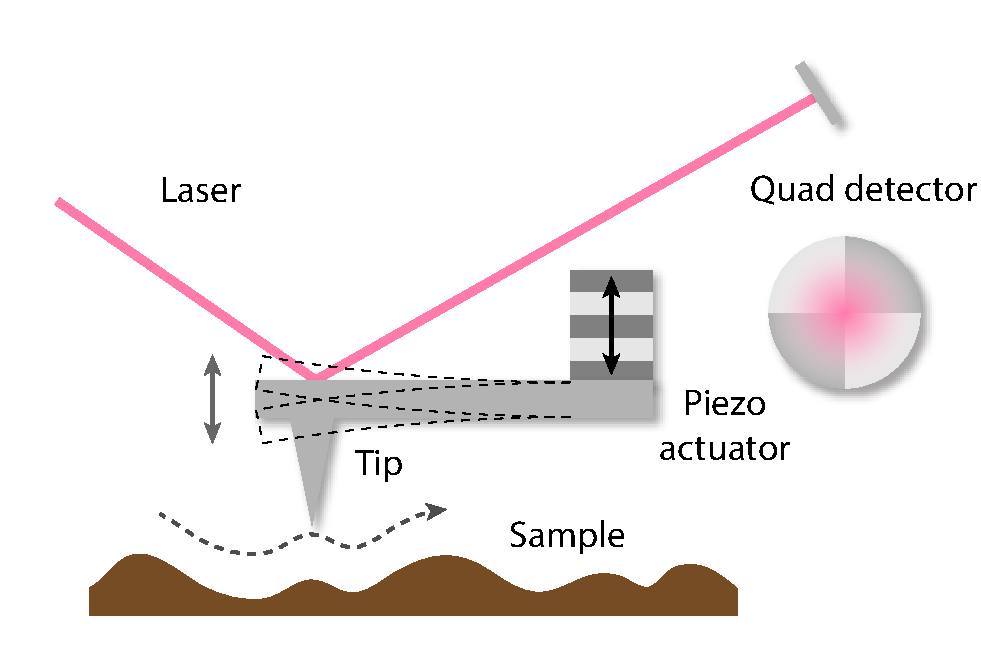
\includegraphics[width=0.6\textwidth]{Drawing/NonContactAFM.pdf}
	\caption{AFM Contact mode. The tip is kept at a distance from the sample so that the interaction is always attractive. The tip does not have direct contact with the sample during the scanning.}
	\label{FIG:NonContactAFM}
\end{figure}

\subsection{Magnetic force microscopy}
\label{SEC:AFMMFM}

When the tip is coated with ferromagnetic materials (e.g. Co, Fe), the AFM is able to measure the magnetic interaction with magnetic force microscopy (MFM). Similar to AC mode, the tip is driven by an oscillating AC voltage close to the resonance frequency (about 100 kHz in my experiments), and the change of interaction is monitored by the amplitude $A$ and phase $\theta$ of the differential voltage on quad detector. The challenge of MFM is that the magnetic and Van der Waals interactions are coupled together. The two-pass technique is used to solve this problem, considering that Van der Waals interaction is short-ranged and decays much faster than the magnetic interaction. First, the tip scans the sample close to the surface, and measures the topography. Second, the tip is lifted and maintained at a constant distance (such as 50 nm) from the sample surface using the height information obtained from the previous scan, so that the Van der Waals interaction is negligible, and the spatial gradient of magnetic force can be measured\cite{hartmann1999magnetic}:
\begin{equation}
%\begin{split}
\label{EQN:MFM}
\Delta A \approx \frac{2 A_0 Q}{3\sqrt{3k}} \cdot \frac{\partial F_z}{\partial z}, \ \ \ \
\Delta \phi \approx \frac{Q}{k} \cdot \frac{\partial F_z}{\partial z}, \ \ \ \
\Delta f \approx -\frac{f_0}{2k} \cdot \frac{\partial F_z}{\partial z}, 
%\end{split}
\end{equation}
where $\Delta A$, $\Delta \phi$ and $\Delta f$ are the change of amplitude, phase and resonance frequency; $A_0$ and $f_0$ are the original amplitude and frequency; $Q$ and k are the resonance quality factor and cantilever spring constant. $\partial F_z/\partial z$ is the spatial gradient of magnetic force. 

Like contact and AC mode of AFM, the resolution of MFM is limited by the tip radius of curvature. Ferromagnetic coating of the MFM tip is about 40 nm in my experiments, so the resolution is in the same order of magnitude. 

The advantage of MFM is that, the resolution and sensitivity is higher than other methods such as magneto-optical effect imaging. Also, like contact and AC mode AFM imaging, MFM does not require special treatment on the sample. The downside of MFM is that the imaging speed is limited by the raster scanning speed. The two-pass method takes twice as long as usual AFM AC scanning. Also, as equation (\ref{EQN:MFM}) shows, MFM signal is not determined by the absolute value of magnetic force, but is proportional to the spatial gradient of the force $\partial F_z/\partial z$, therefore the scanning speed would also affecting the signal. The field from the AFM tip can also affect the magnetic dipoles on the sample, and MFM image can change after each scan. Other long range interaction such as coulomb interaction cannot be eliminated by the two-pass method, and need to be taken care of. More details are discussed in the next chapter. In spite of these disadvantages, the MFM is still a power tool to study surface magnetism for its robustness and simplicity of operations.

\begin{figure}[h!]
	\centering
	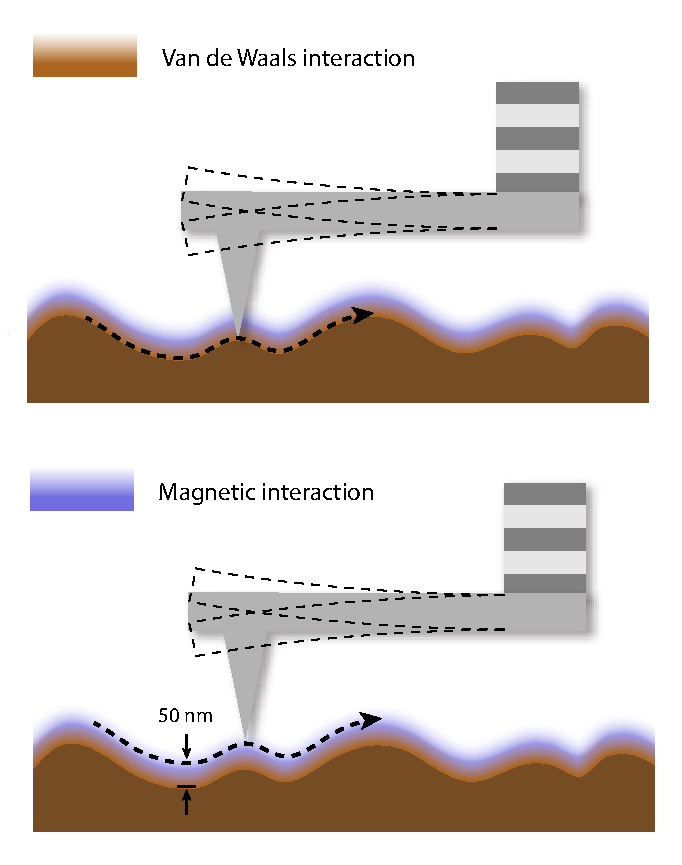
\includegraphics[width=0.5\textwidth]{Drawing/MFM.pdf}
	\caption{MFM mode. The first scan is close to the sample surface, so that the topographical information can be obtained. In the second scan the tip is lifted to a constant distance from the sample surface, so that the Van der Waals interaction is negligible and only the long-ranged magnetic interaction is measured.}
	\label{FIG:MFM}
\end{figure}

\subsection{Piezoresponse force microscopy}

The high sensitivity and extendability of AFM make it a versatile tool to measure different types of interactions between the tip and sample. One important variant is piezoresonse force microscopy (PFM). Piezoelectric effect is the phenomenon when an external stress or strain is applied to a piezoelectric material, the deformation will induce electric dipole moments and build up an internal electric potential across the sample. Inversely, the external electric field can also induce mechanical deformation. Depending on the properties of the material, the deformation can be either expansion or contraction. The effect can be described with
$$
X_i = d_{ki}E_k,
$$
where $X_i$ is the strain tensor, $d_{ki}$ is the piezoelectric tensor and $E_k$ is the electric field. For a tetragonal system, 
$$
\begin{bmatrix}
X_{1} \\
X_{2} \\
X_{3} \\
X_{4} \\
X_{5} \\
X_{6}
\end{bmatrix} =
\begin{bmatrix}
0 & 0 & d_{31} \\
0 & 0 & d_{32} \\
0 & 0 & d_{33} \\
0 & d_{15} & 0 \\
d_{15} & 0 & 0 \\
0 & 0 & 0
\end{bmatrix}
\begin{bmatrix}
E_{1} \\
E_{2} \\
E_{3}
\end{bmatrix}
$$
When a field is applied in $E_3$ direction, the resulting non-zero strain terms are $X_1 = d_{31}E_3$, $X_2 = d_{32}E_3$ and $X_3 = d_{33}E_3$. Therefore, an electric field in the c-axis of the crystal will cause elongation in the c-axis and contraction in the other two orthogonal directions, or vice versa. The piezoresponse of sample can bring insights of the sample properties such as carrier concentration\cite{}, ferroelectric domain orientation\cite{}, domain boundary\cite{}, etc. The piezoresponse of the LAO/STO system can be used to characterize the carrier density change on the interface. More details will be discussed in the following section.

\begin{figure}[p]
	\centering
	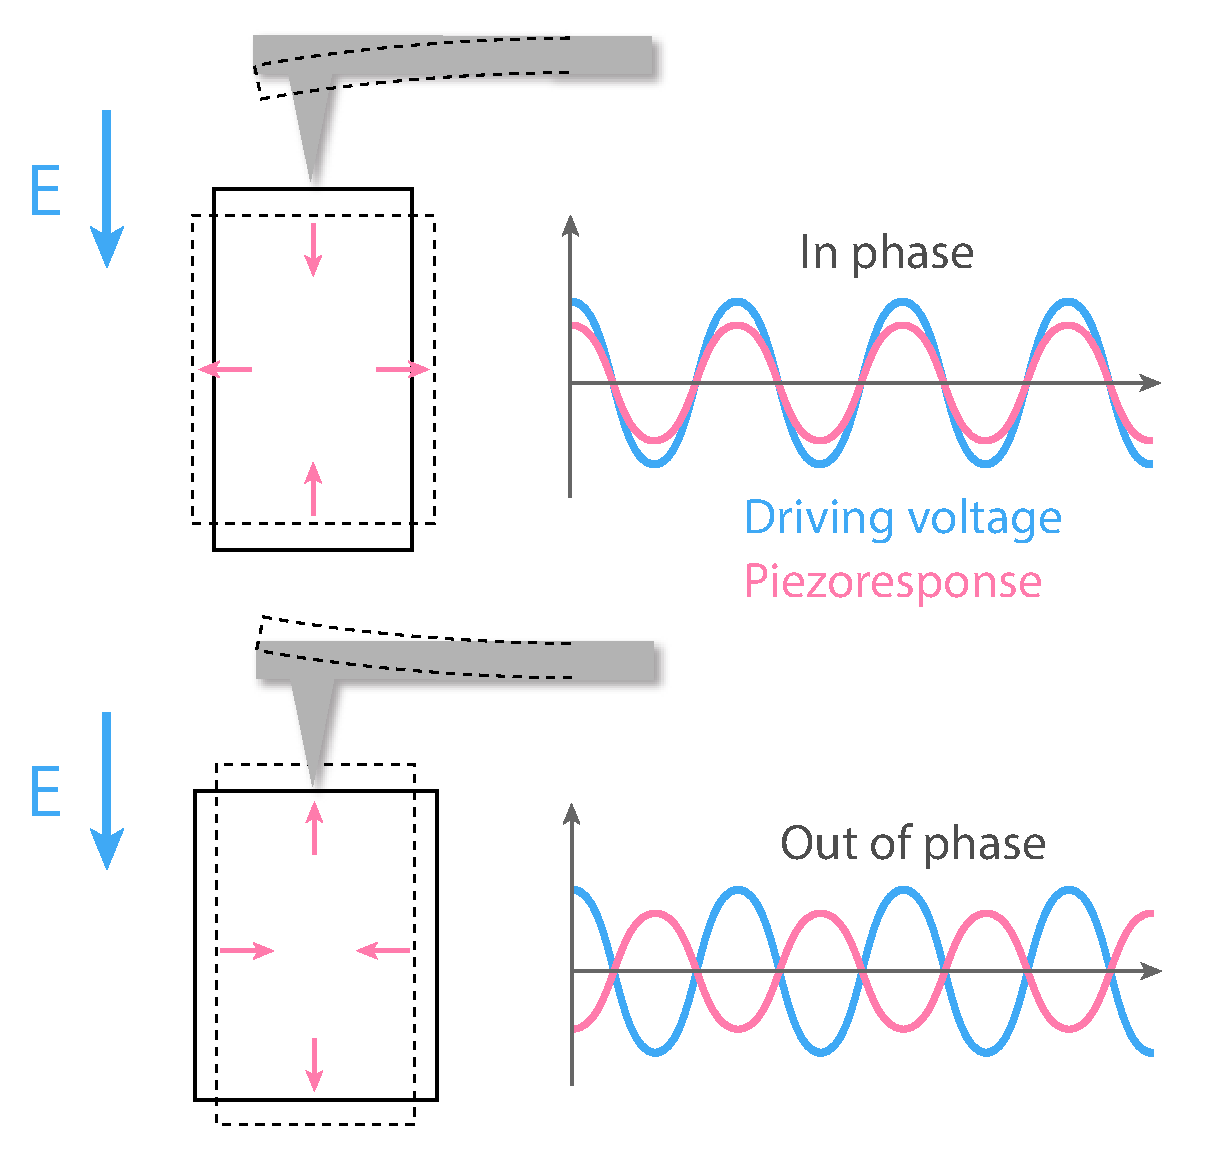
\includegraphics[width=0.7\textwidth]{Drawing/PFM.pdf}
	\caption{PFM measurement. The external electric field is applied on the sample through a conductive tip. The sample deforms and slightly bend the tip, and the deformation signal is monitored with a quad detector (not shown). If the sample contract in the direction of the field, the deformation signal is in phase with the driving voltage (above); if the sample elongate in the direction of the field, the signal would be out of phase with the driving voltage (below).}
	\label{FIG:PFM}
\end{figure}

In PFM measurement, a conductive tip made of doped silicon or coated with metal is in contact with the sample and a sinusoidal voltage signal is applied to the tip. For a sample with piezoresponse, the electric field will cause a deformation of the sample topography sinusoidal in time. Since the sample is in contact with the tip, the topographical change of sample will cause slight change of tip deformation and the change is recorded by the differential voltage on the quad detector. The sample deformation is usually in the order of 10 pm/V (e.g. 85.6 pm/V for BaTiO$_3$\cite{}). Therefore, PFM signal is measured with lock-in technique for the best signal-to-noise ratio. As shown in Figure \ref{FIG:PFM}, If the sample contract in the direction of the electric field, the piezoresponse signal will be in phase with the electric signal; if the sample elongate in the direction of the field, the signal will be out of phase.

\subsection{LAO/STO nano-device c-AFM lithography}
\label{SEC:AFMLitho}

Other than performing surface characterization, the main application of AFM in our lab is to create nano-scale structures on the interface of LAO/STO. As discussed in Section \ref{}, the ``water-cycle'' mechanism\cite{bi2010water} and surface protonation\cite{} are central for the reversible AFM lithography on LAO/STO interface. In contact mode, the AFM tip is in direct contact with the LAO/STO sample surface. When a positive voltage is applied to the conductive AFM tip, and $V_\mathrm{tip} > +6$V\cite{cen2008nanoscale}, the electric field from the tip will dissociate the water molecules between the tip and sample surface, and leaves a trace of proton, as the tip scans through the LAO surface. 

\begin{figure}[p]
	\centering
	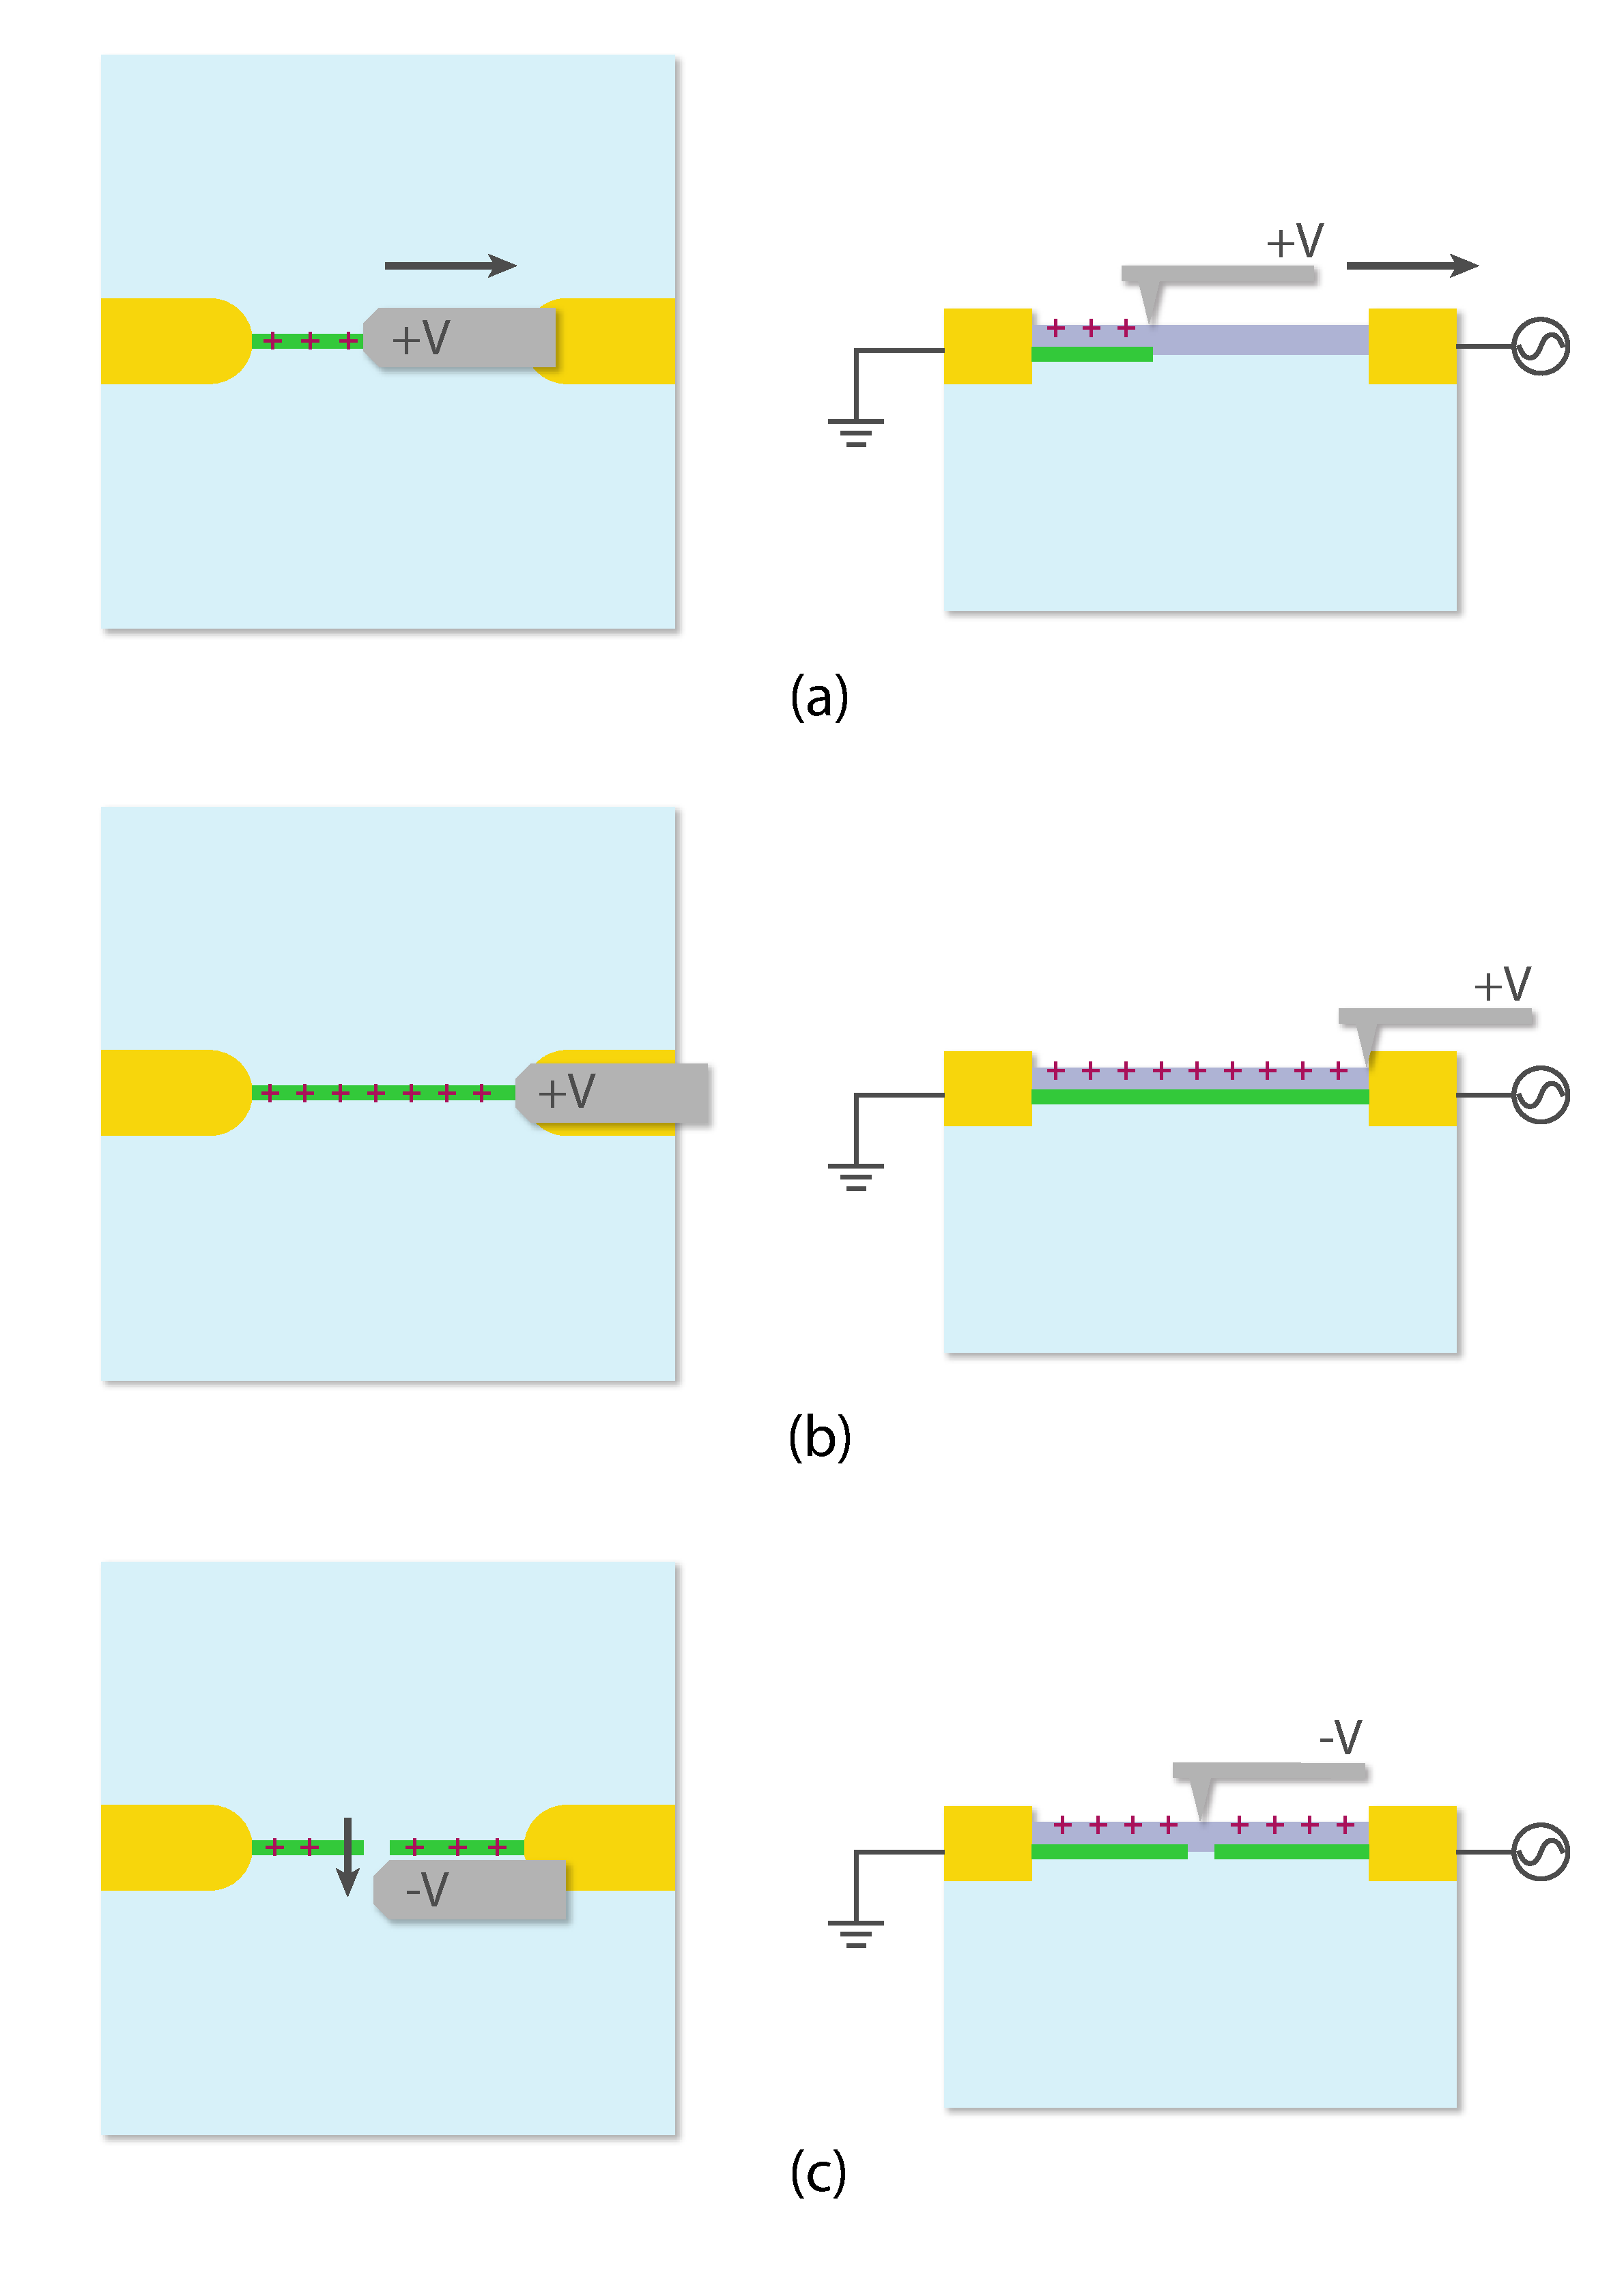
\includegraphics[width=.80\textwidth]{Drawing/Lithography.pdf}
	\caption{AFM lithography on LAO/STO. (a)(b) The AFM is set in contact mode. A positive bias voltage is applied to the tip. A trace of proton is left on the path of AFM tip, and 2DEG is formed underneath the path. Conductivity of the two interface electrodes are monitored, and a conductance jump will be observed once a closed loop is formed. (c) A negative voltage can remove the proton and cut the nanowire previously written.}
	\label{FIG:Lithography}
\end{figure}

As shown in Figure \ref{FIG:Lithography}, the golden regions are a pair of electrodes connected to the LAO/STO interface. An AC voltage of $\pm100$ mV is applied to one electrode, while the other one is grounded. Before the c-AFM lithography starts, the interface between the two electrodes is insulating. The current between them is monitored in real-time as the c-AFM tip scans through the surface (zero before lithography starts). A positive voltage is applied, and protons are dissociated from the water meniscus and left behind the tip (plus signs in the Figure). 2DEG is formed under the protonated region and makes the interface conductive (green region). Once the two electrodes are connected by the conductive channel, a conductance jump can be observed. When a negative voltage on the tip is applied, the protons will be removed from the surface and make the interface insulating again. A typical resistance of the nanowire right after the writing is about 200 k$\Omega$/$\mu$m, and the width is in the same order of magnitude as the c-AFM tip\cite{cen2008nanoscale}.

The sample is patterned in such a way that I can do AFM lithography and electrical measurement in real-time. Figure \ref{FIG:Regular} show the pattern of a typical LAO/STO sample for c-AFM lithography. The dimension of the sample is 5 mm $\times$ 5 mm. There are two layers of metals. The blue layer is in direct contact with the LAO/STO interface. The sample is first etched with Ar ion mill and the etched areas are backed-filled with 4 nm of Ti and 25 nm of Au (as discussed in \ref{SEC:IonMilling}). The orange regions are for electrical connections and wire-bonding. 4 nm of Ti and 50 nm of Au are directly coated on the LAO surface without etching. The orange crosses on the corners indicate the corners of the sample. the blue crosses and triangle are guidance for alignment. The zoomed-in image shows the region where c-AFM lithography is performed. The patterns are written inside the 20 $\mu$m $\times$ 20 $\mu$m area, and connected with the interface electrodes.

% image of the conductance jump
% image of the interface of measurement
% PFM image of LAO/STO nanowire

\begin{figure}[p]
	\centering
	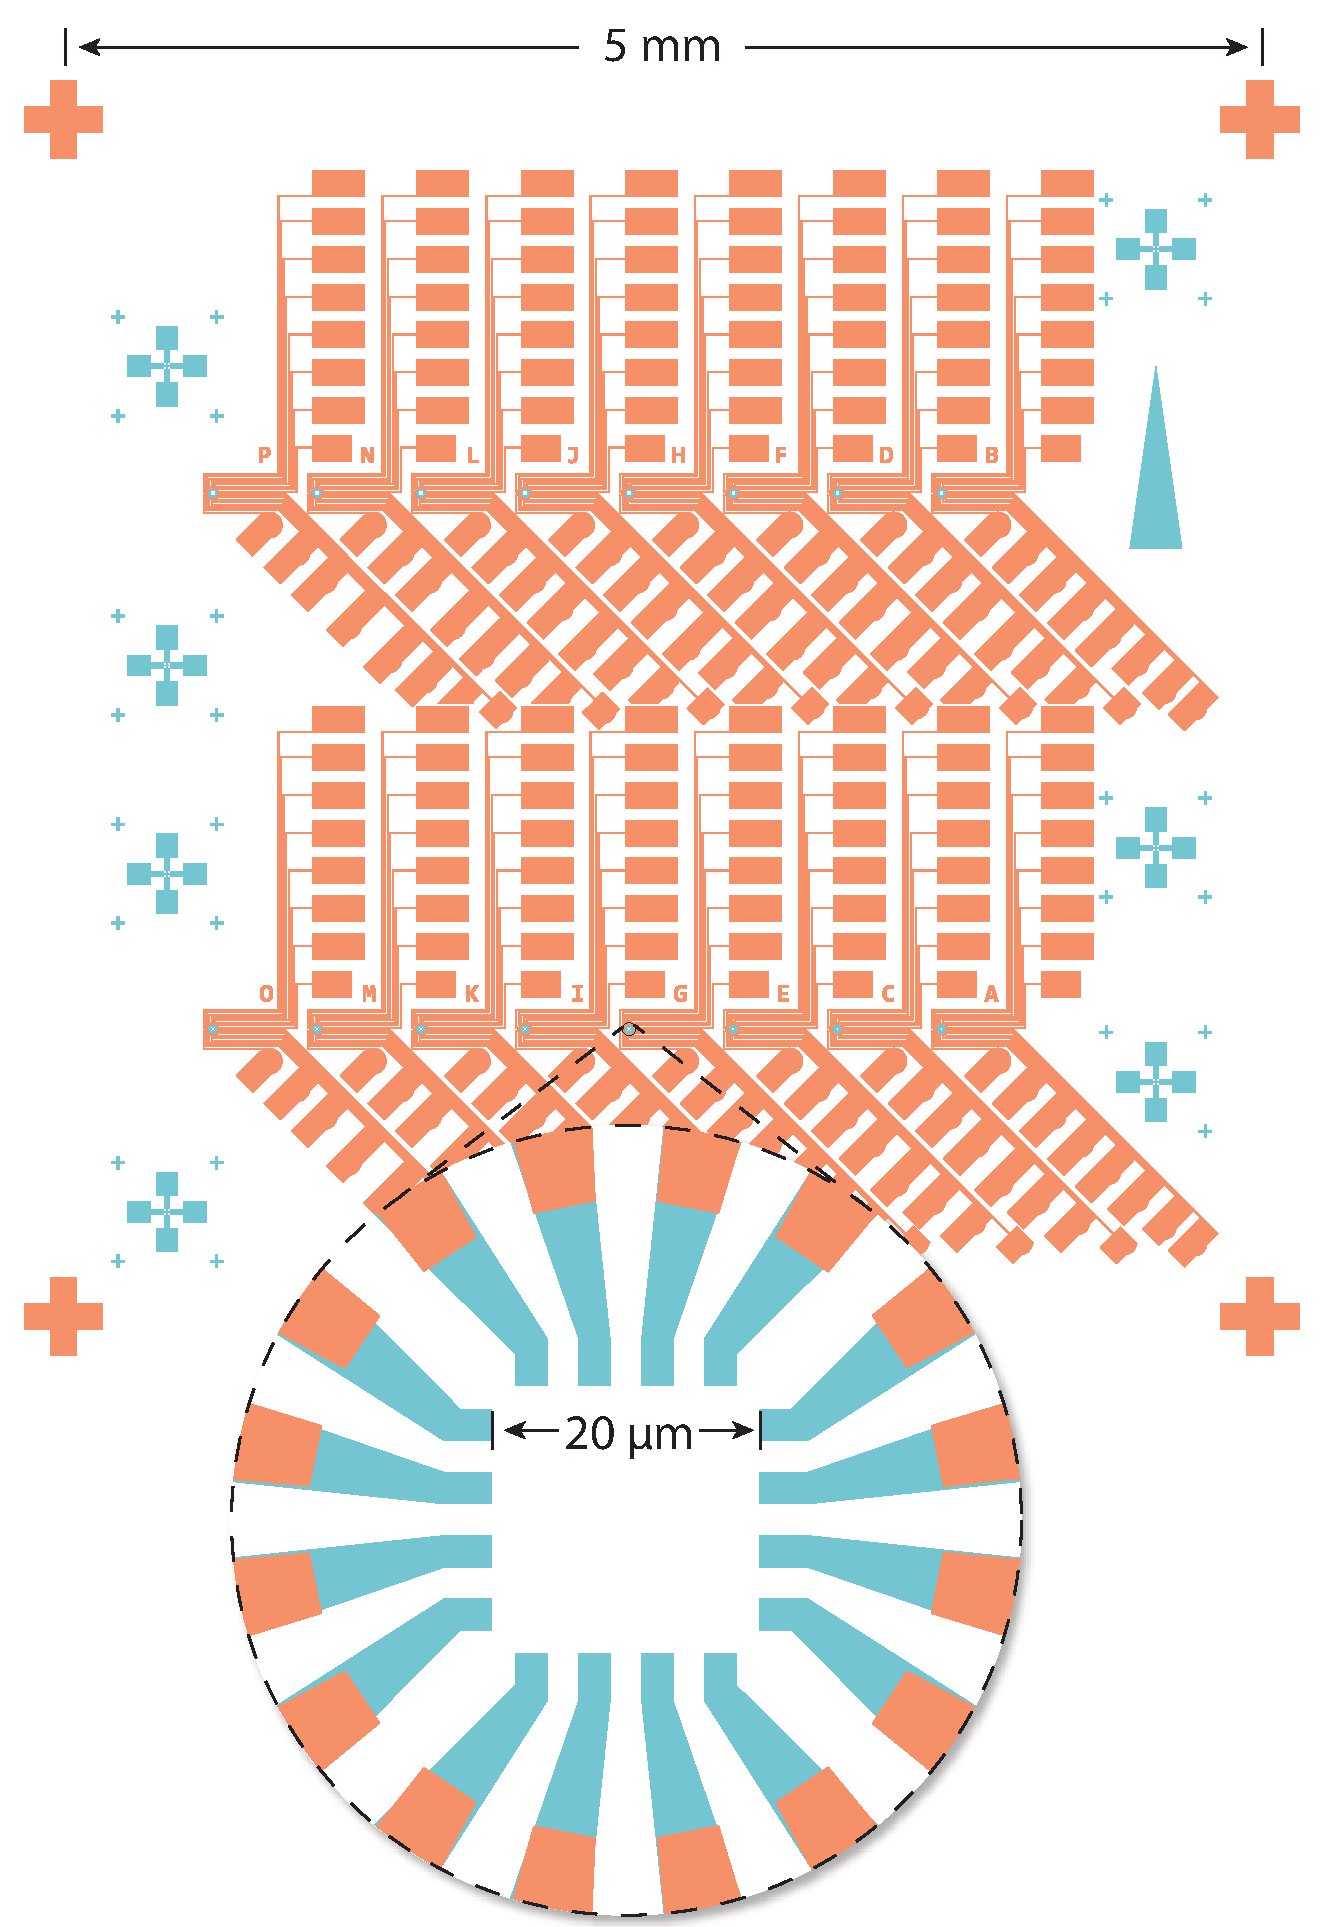
\includegraphics[width=1\textwidth]{Drawing/Regular.pdf}
	\caption{LAO/STO sample pattern for c-AFM lithography. The sample size is 5 mm $\times$ 5 mm. Canvas are 20 $\mu$m squares.}
	\label{FIG:Regular}
\end{figure}

%\section{Electric signal measurement}

%The electrical signal (voltage, current, etc) measured in my experiments are 

%\subsection{Lock-in amplifier}

%\subsection{Virtual lock-in}

%\subsection{IV-curve measurement}

%\subsection{Probe station}

\section{Graphene/LAO/STO device fabrication}

Current state-of-the-art high quality graphene devices are fabricated from mechanically transferred exfoliated graphene encapsulated with hexagonal boron nitride (h-BN)\cite{dean2010naturenano}, where the mean-free-path of the electron can exceed the dimension of the device\cite{Novoselovaac9439} (tens of micrometers). For applications requiring an arbitrary substrate and graphene shape like my experiment, graphene grown from CVD method and transfer in liquid (``wet-transfer'') is preferred. The basic idea of wet-transfer is to use wet chemical etchant such as nitric acid, hydrochloric acid, FeCl$_3$ or ammonium persulfate (AP) to etch away the metal substrate while the graphene is floating on the liquid surface. The graphene is then scooped out and rinsed in DI-water for several times while floating on water. The substrate is then immersed in the DI-water and used to catch the graphene piece from the bottom. Conventionally, the wet-transfer needs polymers like poly(methyl methacrylate) (PMMA) a scaffold layer to support  graphene on the liquid surface before it is transferred onto the substrate\cite{li2009transfer, reina2008transferring, reina2008large}. The PMMA is then patterned with deep UV exposure or e-beam lithography, so that graphene can be etched in to the designed shape. In the end the PMMA is cleaned with organic solvent. The procedure of using PMMA to transfer and pattern graphene shown in Figure \ref{FIG:PMMATransfer}. 

\begin{figure}[p]
	\centering
	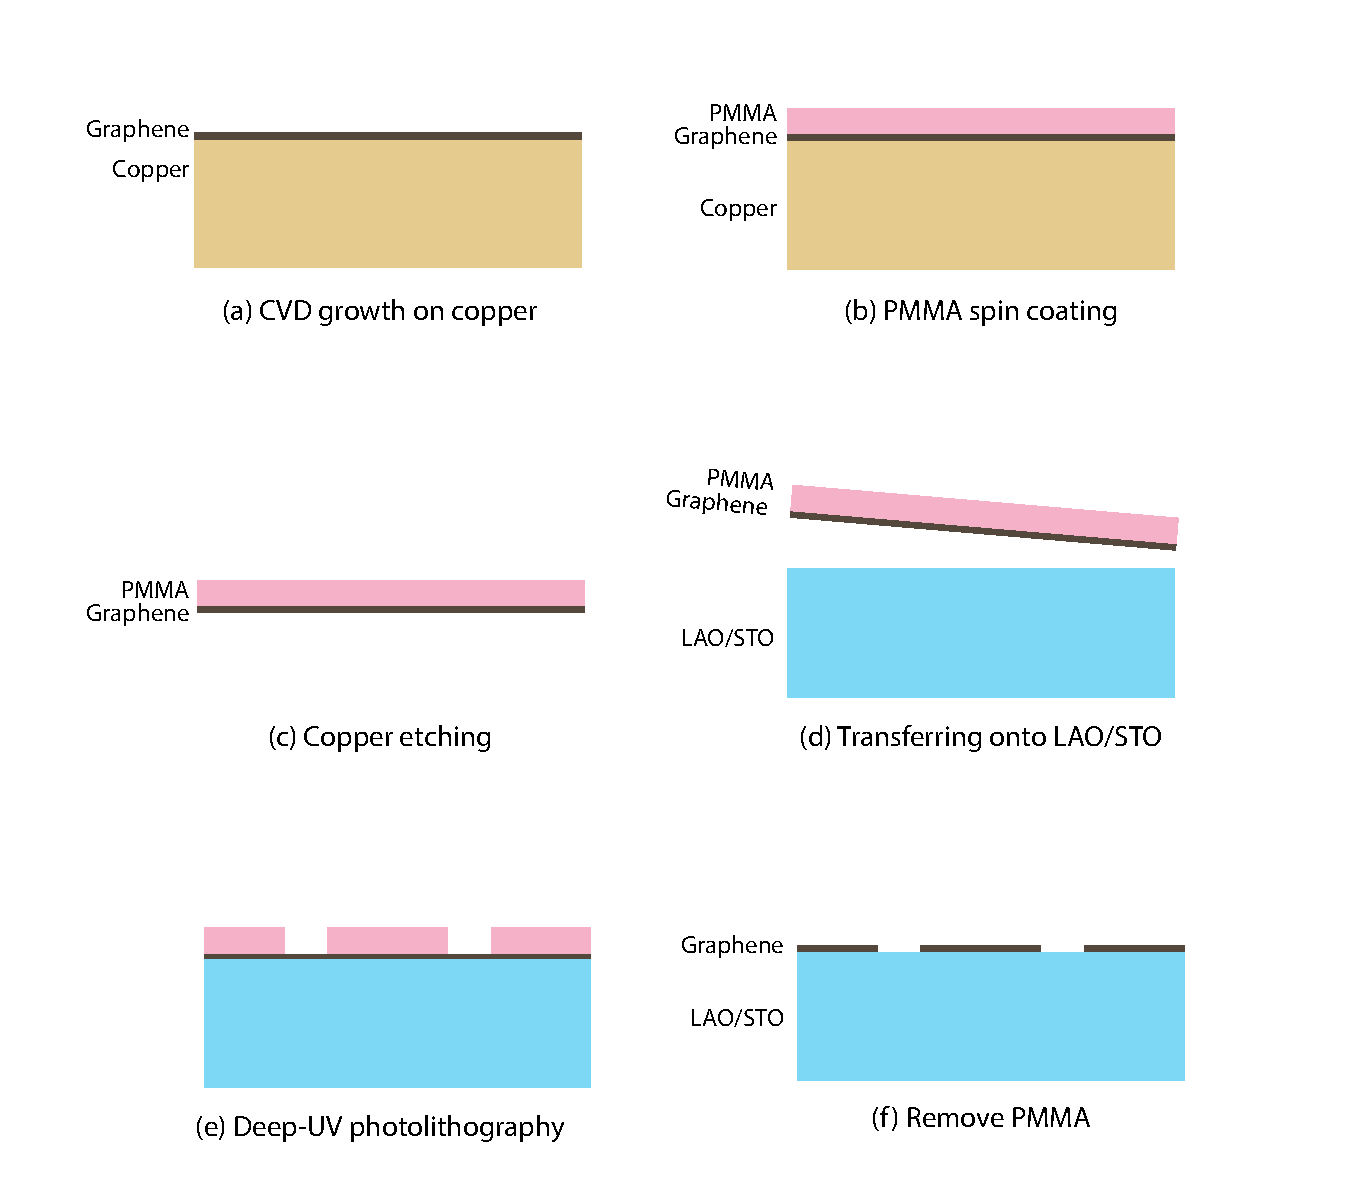
\includegraphics[width=.90\textwidth]{Drawing/PMMATransfer.pdf}
	\caption{CVD graphene transfer and patterning with PMMA. (a) Graphene is grown on copper with CVD. (b) PMMA is spin-coated onto graphene surface. (c) Copper is etched chemically, while graphene floats on the liquid surface. (d) Graphene is transferred onto LAO/STO, using PMMA as a supporting layer. (d) PMMA is patterned with deep-UV lithography. (f) Graphene is etched with oxygen plasma and then PMMA is removed with organic solvent.}
	\label{FIG:PMMATransfer}
\end{figure}

The issue with PMMA as transfer medium is that, the residual PMMA is known to be a source of electron scattering, and would significantly reduce the electron mobilities\cite{pirkle2011effect, lin2011graphene, cheng2011toward}. Annealing the sample in H$_2$/Ar environment proves to partially remove the residue, but the process can also introduce structural defects to graphene\cite{lin2011graphene}, or increase coupling between graphene and the substrate and result in extrinsic doping and deterioration of mobility\cite{cheng2011toward}. 
\\

\begin{figure}[h!]
	\centering
	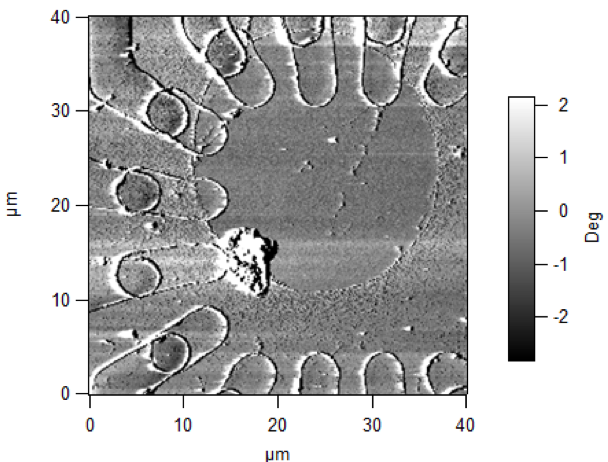
\includegraphics[width=0.60\textwidth]{Drawing/PMMAResidue.png}
	\caption{AFM phase image of graphene on LAO/STO, transferred with PMMA. The circular region is graphene. Particles can be seen outside graphene, on LAO/STO surface. Other features are the metal electrodes for grahene and interface contact.}
	\label{FIG:PMMAResidue}
\end{figure}

Another drawback of using PMMA as a transfer medium is that LAO/STO substrate is susceptible to PMMA contaminants. Figure \ref{FIG:PMMAResidue} shows the AFM AC phase image of  LAO/STO with a graphene piece transferred and patterned with PMMA. The inside the circular region is graphene. On the LAO/STO surface, contamination particles can be seen. Many experiments in my project require tuning the 2D electron gas on the interface of LAO/STO with c-AFM (will be discussed in Section \ref{SEC:AFM}). Most of the LAO/STO samples were found to lost the interface tunability after the graphene transfer with PMMA. 

A replacement for PMMA is a type of perfluoropolymer Hyflon from Solvay. Our collaborator Brian D'Urso has used Hyflon for hydrodynamic experiment, and suggested it might work as a perfect protection layer for graphene. Hyflon is a type of perfluorinated polymer (similar to Teflon), and is highly hydrophobic and chemically stable. Hyflon has been reported to be widely used in membrane applications such as fuel cells, due to the inertness of C-F bonds\cite{arcella2005hyflon, merlo2007membrane, zhang2012recent}. It has also been reported that the Hyflon membrane between graphene and substrates like SiO$_2$ can reduce the extrinsic p-type doping in graphene by preventing water molecule adsorption to the dangling bonds on the substrates\cite{mattevi2012solution}. It means that, unlike PMMA that leaves residue and deteriorate graphene quality, Hyflon can actually preserve the graphene while used as a transfer medium. Hyflon is also high selectivity to solvent. Most of the organic or inorganic solvent such as acetone, IPA or DI-water cannot dissolve Hyflon, which makes it a perfect protection layer for graphene. 

The commercially available Hyflon is in power form. It is only soluble in a few types of perfluorinated solvent. In my experiment I used FC-40 to make Hyflon solutions. There are different types of Hyflon available, mainly Hyflon AD 40 and Hyflon AD 60, with different molecular weights and phase transition temperature. I have tested both types, and found that graphene transferred with Hyflon AD 60 has higher quality. Although AD 40 has smaller molecular weight and easier to be dissolved, the sample soft-baking temperature is higher than the phase transition temperature of AD 40, and would cause cross-linking of the polymer chains. This makes Hyflon AD 40 hard to be removed and affects graphene quality as a result. 

\subsection{Overview of the Hyflon transfer method}

\begin{figure}[p]
	\centering
	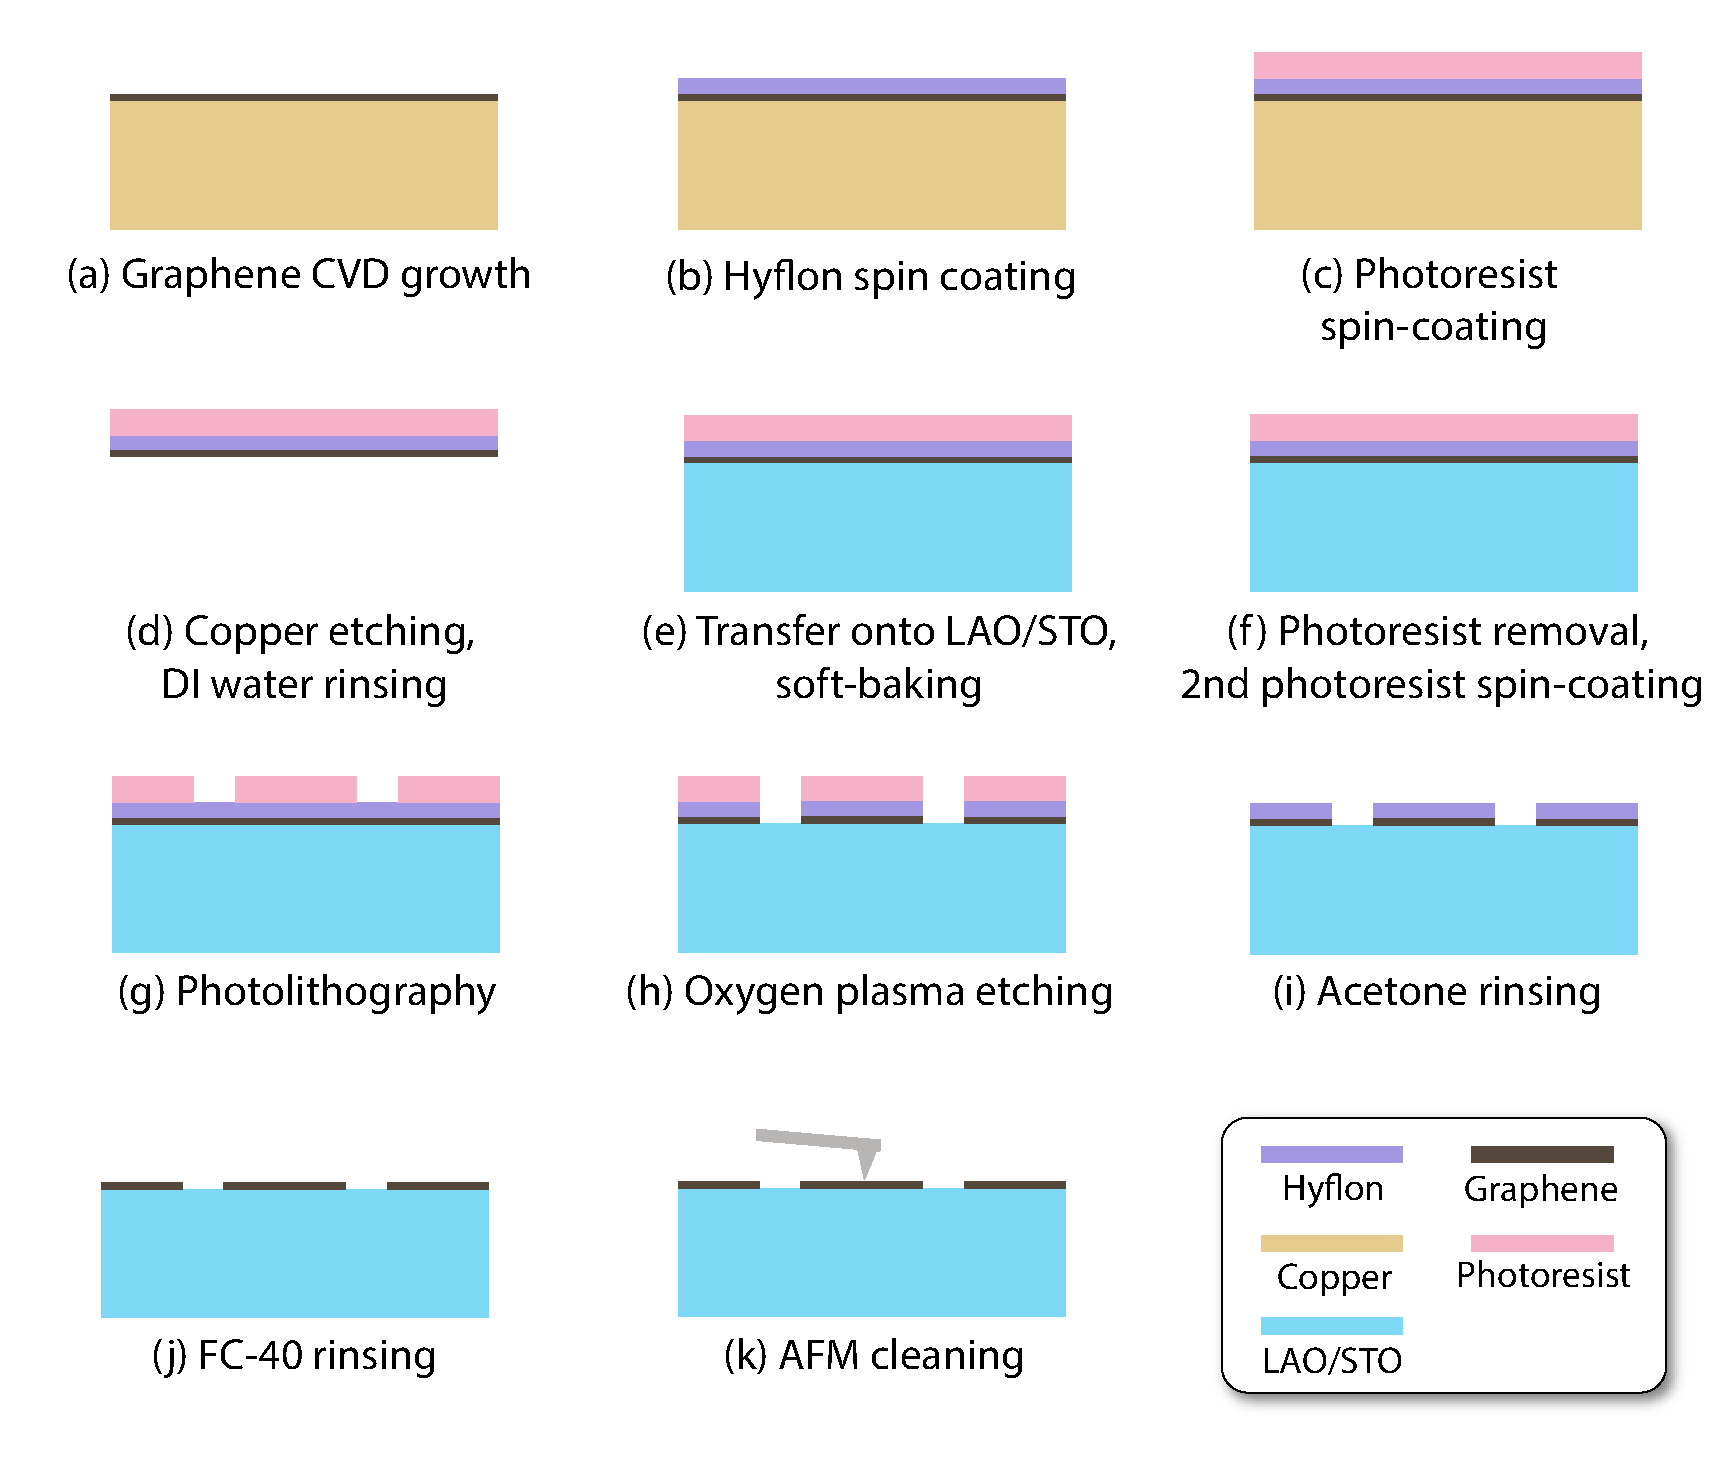
\includegraphics[width=1.0\textwidth]{Drawing/HyflonTransfer.pdf}
	\caption{Hyflon transfer and patterning procedure. (a) Graphene is grown with CVD on a copper substrate. (b) Hyflon in spin-coated on graphene. (c) A layer of photoresist is coated on Hyflon as a supporting layer for wet-transfer. (d) Copper substrate is etched with ammonium persulphate; graphene is rinsed in DI-water for several times. (e) Graphene is transferred onto LAO/STO surface. (f) Photoresist for transfer assistance is removed; another layer of photoresist is coated. (g) Standard UV photolithography. (h) Oxygen plasma etching on the excessive graphene. (i) Photoresist removal with acetone. (j) Hyflon removal with FC-40. (k) Residue particle cleaning with AFM.}
	\label{FIG:HyflonTransfer}
\end{figure}

The procedure for graphene transfer with Hyflon is similar to the PMMA transfer method. As shown in Figure \ref{FIG:HyflonTransfer}, the graphene on copper is spin coated with Hyflon. The Hyflon film is only 50 nm, therefre a second supporting layer, photoresist, is spin-coated on top of the Hyflon. The copper is etched with ammonium persulphate while graphene with Hyflon and photoresist floats on the surface of chemical. The graphene is then rinsed 4 to 5 times and then transferred onto a pre-patterned LAO/STO substrate, and soft-baked to remove the DI water between graphene and LAO. The photoresist is then removed, and another layer of photoresist is spin-coated. The sample is patterned into Hall bars with standard photolithography. Excessive graphene is etched away with oxygen plasma, along with the Hyflon covering it. The patterned graphene/LAO/STO sample is rinsed with acetone to remove the photoresist, and then Hyflon is removed with FC-40. The particles left on the patterned graphene surface is cleaned by AFM in contact mode scans. 

\subsection{Hyflon solution preparation and spin-coating} 

% image of Hyflon in powder form.

Hyflon solutions in FC-40 are made by adding 2.5 grams of Hyflon powder into 100 ml FC-40 (nominally 2.5\%). The solution is shaken at 100 rpm for 48 hours. Before spin-coated on sample, the Hyflon solution needs go through a series of filters of 450 nm, 200 nm and 100 nm in size to remove any undissolved particles. When spin-coated at 3500 rpm, the thickness of Hyflon film is about 50 nm. In the past I also used 0.5\% Hyflon solution and spin-coated at 1000 rpm to make coatings of 50 nm, but it turned out that higher concentration of Hyflon solutions spin-coated at a higher speed would yield more uniform films on graphene samples. 

\subsection{Graphene preparation, copper etching and wet transfer}

\begin{figure}[p]
	\centering
	\includegraphics[width=1.0\textwidth]{Drawing/Transfer.pdf}
	\caption{(a) The graphene with copper foil is cut into squares. The graphene single domains can be seen. (b) copper foil with CVD graphene is fixed onto a silicon wafer as a spin-coating carrier. The edges of the copper foils are carefully sealed with Kapton tape to prevent Hyflon solution leaking into the space between copper and silicon substrate. (c) After the copper is fully etched by ammonium persulfate, the graphene flake with Hyflon and photoresist floats on the surface of the liquid. (d) Graphene transferred onto pre-patterned LAO/STO. Liquid between the graphene LAO is evaporated in an oven or on a hot plate.}
	\label{FIG:Transfer}
\end{figure}

The as-grown CVD graphene is on 100 $\mu$m thick circular copper foil. The LAO/STO substrates that graphene will be transferred on are 5 mm $\times$ 5 mm squares. Therefore, the graphene on copper needs to be cut into 5 mm $\times$ 5 mm shape with a razor blade as shown in Figure \ref{FIG:Transfer}(a). Graphene single domains can be seen in the Figure. The square shape copper foil is then fixed onto a 3'' silicon wafer for spin coating, with Kapton tapes, prepared for Hyflon spin coating. The edges of the graphene need to be carefully sealed, so that the Hyflon solution will not leak into the space between the copper and silicon wafer. In the past, I used to leave the edges open, and the Hyflon will be left on the backside of the copper. After copper etching and graphene transferred onto the LAO/STO, the Hyflon on the backside will be trapped between graphene and substrate and impossible to be removed.

Transferring graphene with only the 50 nm Hyflon proved to be very hard. To address this issue, an additional layer of AZ4210 photoresist is spin-coated on Hyflon. However, since the Hyflon is highly hydrophobic, the photoresist solution cannot stick to the surface and form a film of 2.1$\mu$m thick, as it usually does on hydrophilic surfaces. A mild oxygen plasma etching is performed to modified the Hyflon surface and improve surface hydrophilicity. The parameters of plasma etching need te be carefully tested. Etching will not only change the Hyflon hydrophilicity, but also change the solubility of Hyflon in FC-40. In the last step where Hyflon is removed by FC-40 from graphene, if the previous Hyflon surface treatment is too strong, the modified Hyflon can cross-linked and hard to be fully removed from graphene. In practice, etching the Hyflon for only a few nanometers would drastically improve the hydrophilicity and make photoresist spin-coating possible.

After spin coating, the copper foil is taken off the silicon substrate. 1 mol/L concentration ammonium persulfate ((NH$_4$)$_2$S$_2$O$_8$) DI-water solution is prepared beforehand. Ammonium persulfate is a type of oxidation agent widely used as copper etchant in printed circuit board industry. Compared to other chemicals like ferric chloride, ammonium persulfate does not leave metal ion to graphene, which is critical for experiments on magnetism or transport. The ammonium persulfate solution also needs to go through a 450 nm polymer filter before the copper foil is place on the surface of it. Copper etching usually takes 3-4 hours. 

\begin{figure}[h!]
	\centering
	\includegraphics[width=1.0\textwidth]{Drawing/PreClean.pdf}
	\caption{(a) Without copper substrate backside cleaning, the graphene transferred onto LAO/STO has contaminant trapped. (b) The graphene on LAO/STO is much cleaner if the backside is cleaned.}
	\label{FIG:PreClean}
\end{figure}

After the graphene transferred onto the LAO/STO, the sample is sometimes found dirty, and the contaminants seemed to be introduced by the transfer procedure. AFM scanning showed that the contaminants were trapped between graphene and LAO. One possibility was that the contaminants were the graphene grown on the backside of the copper. When the copper was etched away by ammonium persulfate, the backside graphene did not sinked into the etchant, but transferred with the topside graphene onto the sample and got trapped between graphene and LAO. 

The \emph{two-step etching} procedure can be used instead. After the copper top surface is coated with Hyflon, it is placed on the surface of ammonium persulfate solution and left inside an ultrasonic cleaner for 15 minutes. While the backside of the copper is been etched, it is also scratched by the ultrasound wave so that the backside graphene can be removed. After 15 minutes, the backside is washed by spraying DI-water on it. The graphene on the topside is protected by Hyflon, and will not be affected by the backside cleaning. Then the copper foil is placed back on the surface of ammonium persulfate. After 3--4 hours the copper foil is fully etched, and the graphene with Hyflon and photoresist would float on the surface, as shown in Figure \ref{FIG:Transfer}(c). The gray color of the floating flake is from the AZ4210 photoresist. The dark spot on the lower-left corner of the flake is a piece of contaminant. 

The graphene flake is then scooped out with e mesh and place on the surface of DI-water, repeated for 4--5 times to make sure the ammonium persulfate is washed off the backside of the flake. Then the LAO/STO substrate is immersed in the DI-water where the flake is floating. The substrate is slowly lifted up towards the flake on the liquid surface, and catch the flake when it comes out of the water. The substrate with the graphene flake on surface is then baked in an oven pre-heated to 50$^{\circ}$C, or on a hot plate at 70$^{\circ}$C for 5--10 minutes so that the DI-water between graphene and substrate is evaporated and graphene firmly adheres to LAO (Figure \ref{FIG:Transfer}(d)).

\subsection{Graphene/LAO/STO sample pattern}

The metal electrodes and bonding pads on LAO/STO are patterned before graphene is transferred. Therefore, electrodes are making contacts with graphene from below. The patterns are slightly modified from the one in Section \ref{SEC:AFMLitho}, so that there are electrodes dedicated for making contacts to graphene. As shown in the zoomed-out image in Figure \ref{FIG:GCO}, the graphene Hall bars are located on the canvas for c-AFM lithography. The graphene is in direct contact with the metal electrodes on LAO/STO surface (orange in color), while LAO/STO are in contact with the interface electrodes (blue in color). Therefore, the two layers can be measured separately. 

\begin{figure}[p]
	\centering
	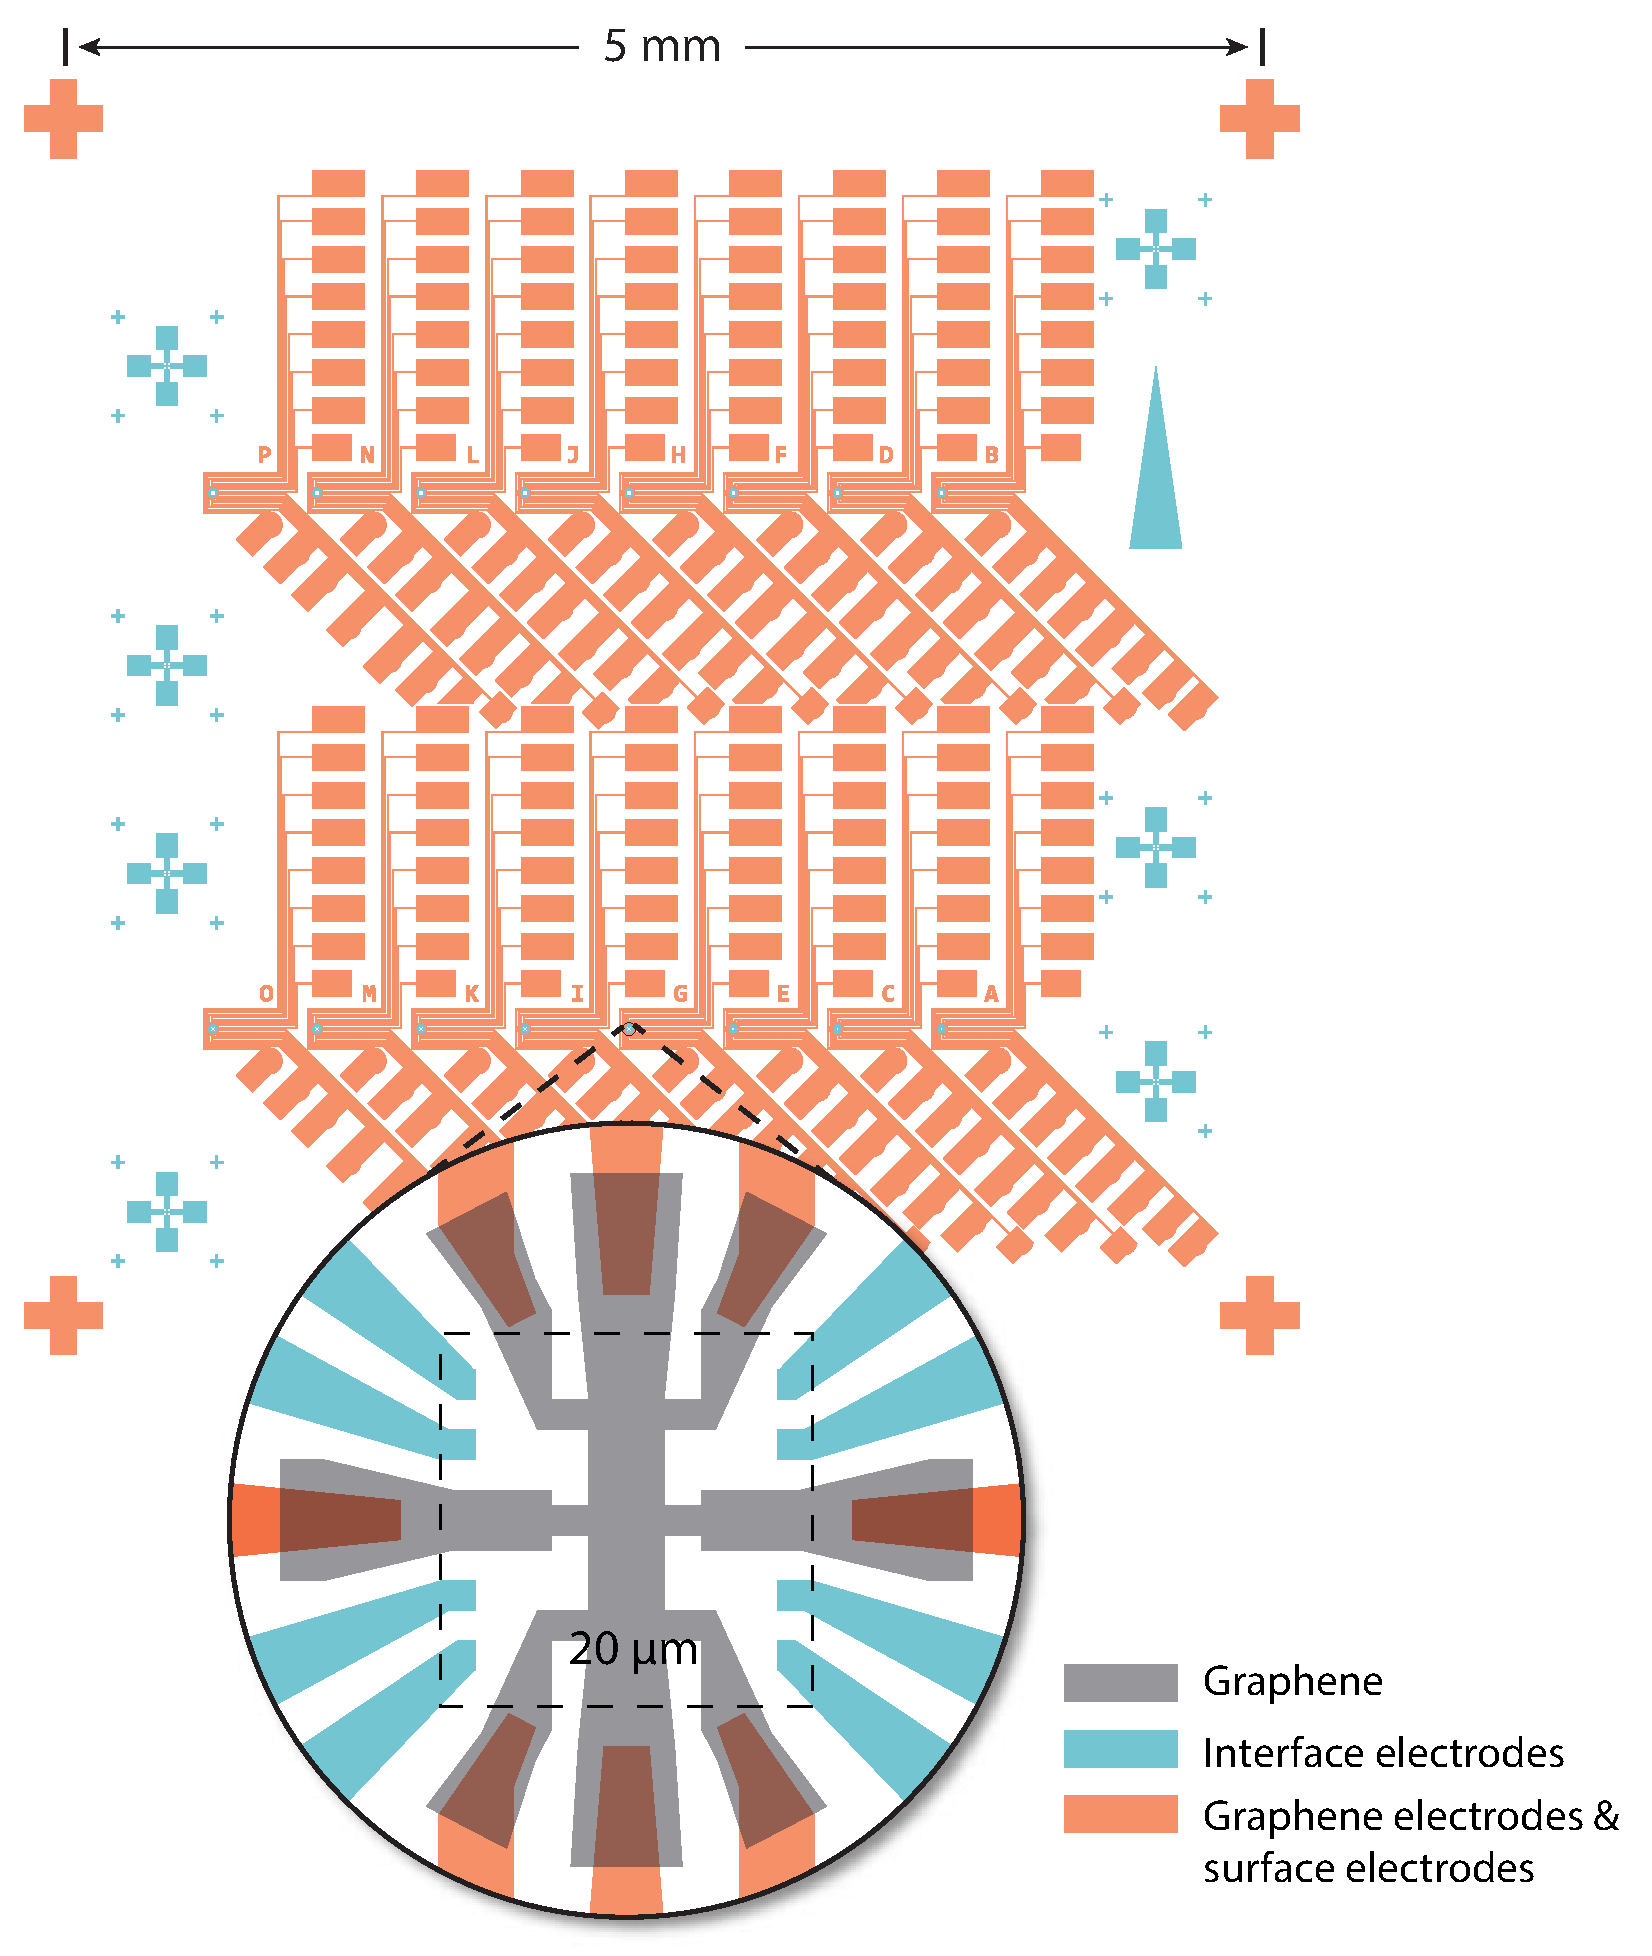
\includegraphics[width=1\textwidth]{Drawing/GCO.pdf}
	\caption{Patterns for graphene/LAO/STO. Two sets of electrodes are patterned separately, for interface and graphene contact.}
	\label{FIG:GCO}
\end{figure}

\subsection{Photolithography and etching}

The graphene transferred onto LAO/STO is patterned with standard UV photolithography, as discussed in Section \ref{SEC:Photolithography}. Although there is already photoresist on graphene flake to assist wet transfer, it needs to be washed off and re-coated, because it is exposed to UV and chemical etchant. Unlike the photolithography for LAO/STO electrodes, patterning graphene into Hall bars need to wash off the photoresist outside of the Hall bars and leave the Hall bar region covered with photoresist, so that the graphene is protected from oxygen plasma etching. The oxygen plasma barrel etcher and RIE proved to be effective for patterning graphene. However, other than the Hyflon and graphene, there are usually contaminant introduced by wet-transfer procedure that need to be cleaned with RIE as well (Figure \ref{FIG:SampleContaminant}). 

\begin{figure}[p]
	\centering
	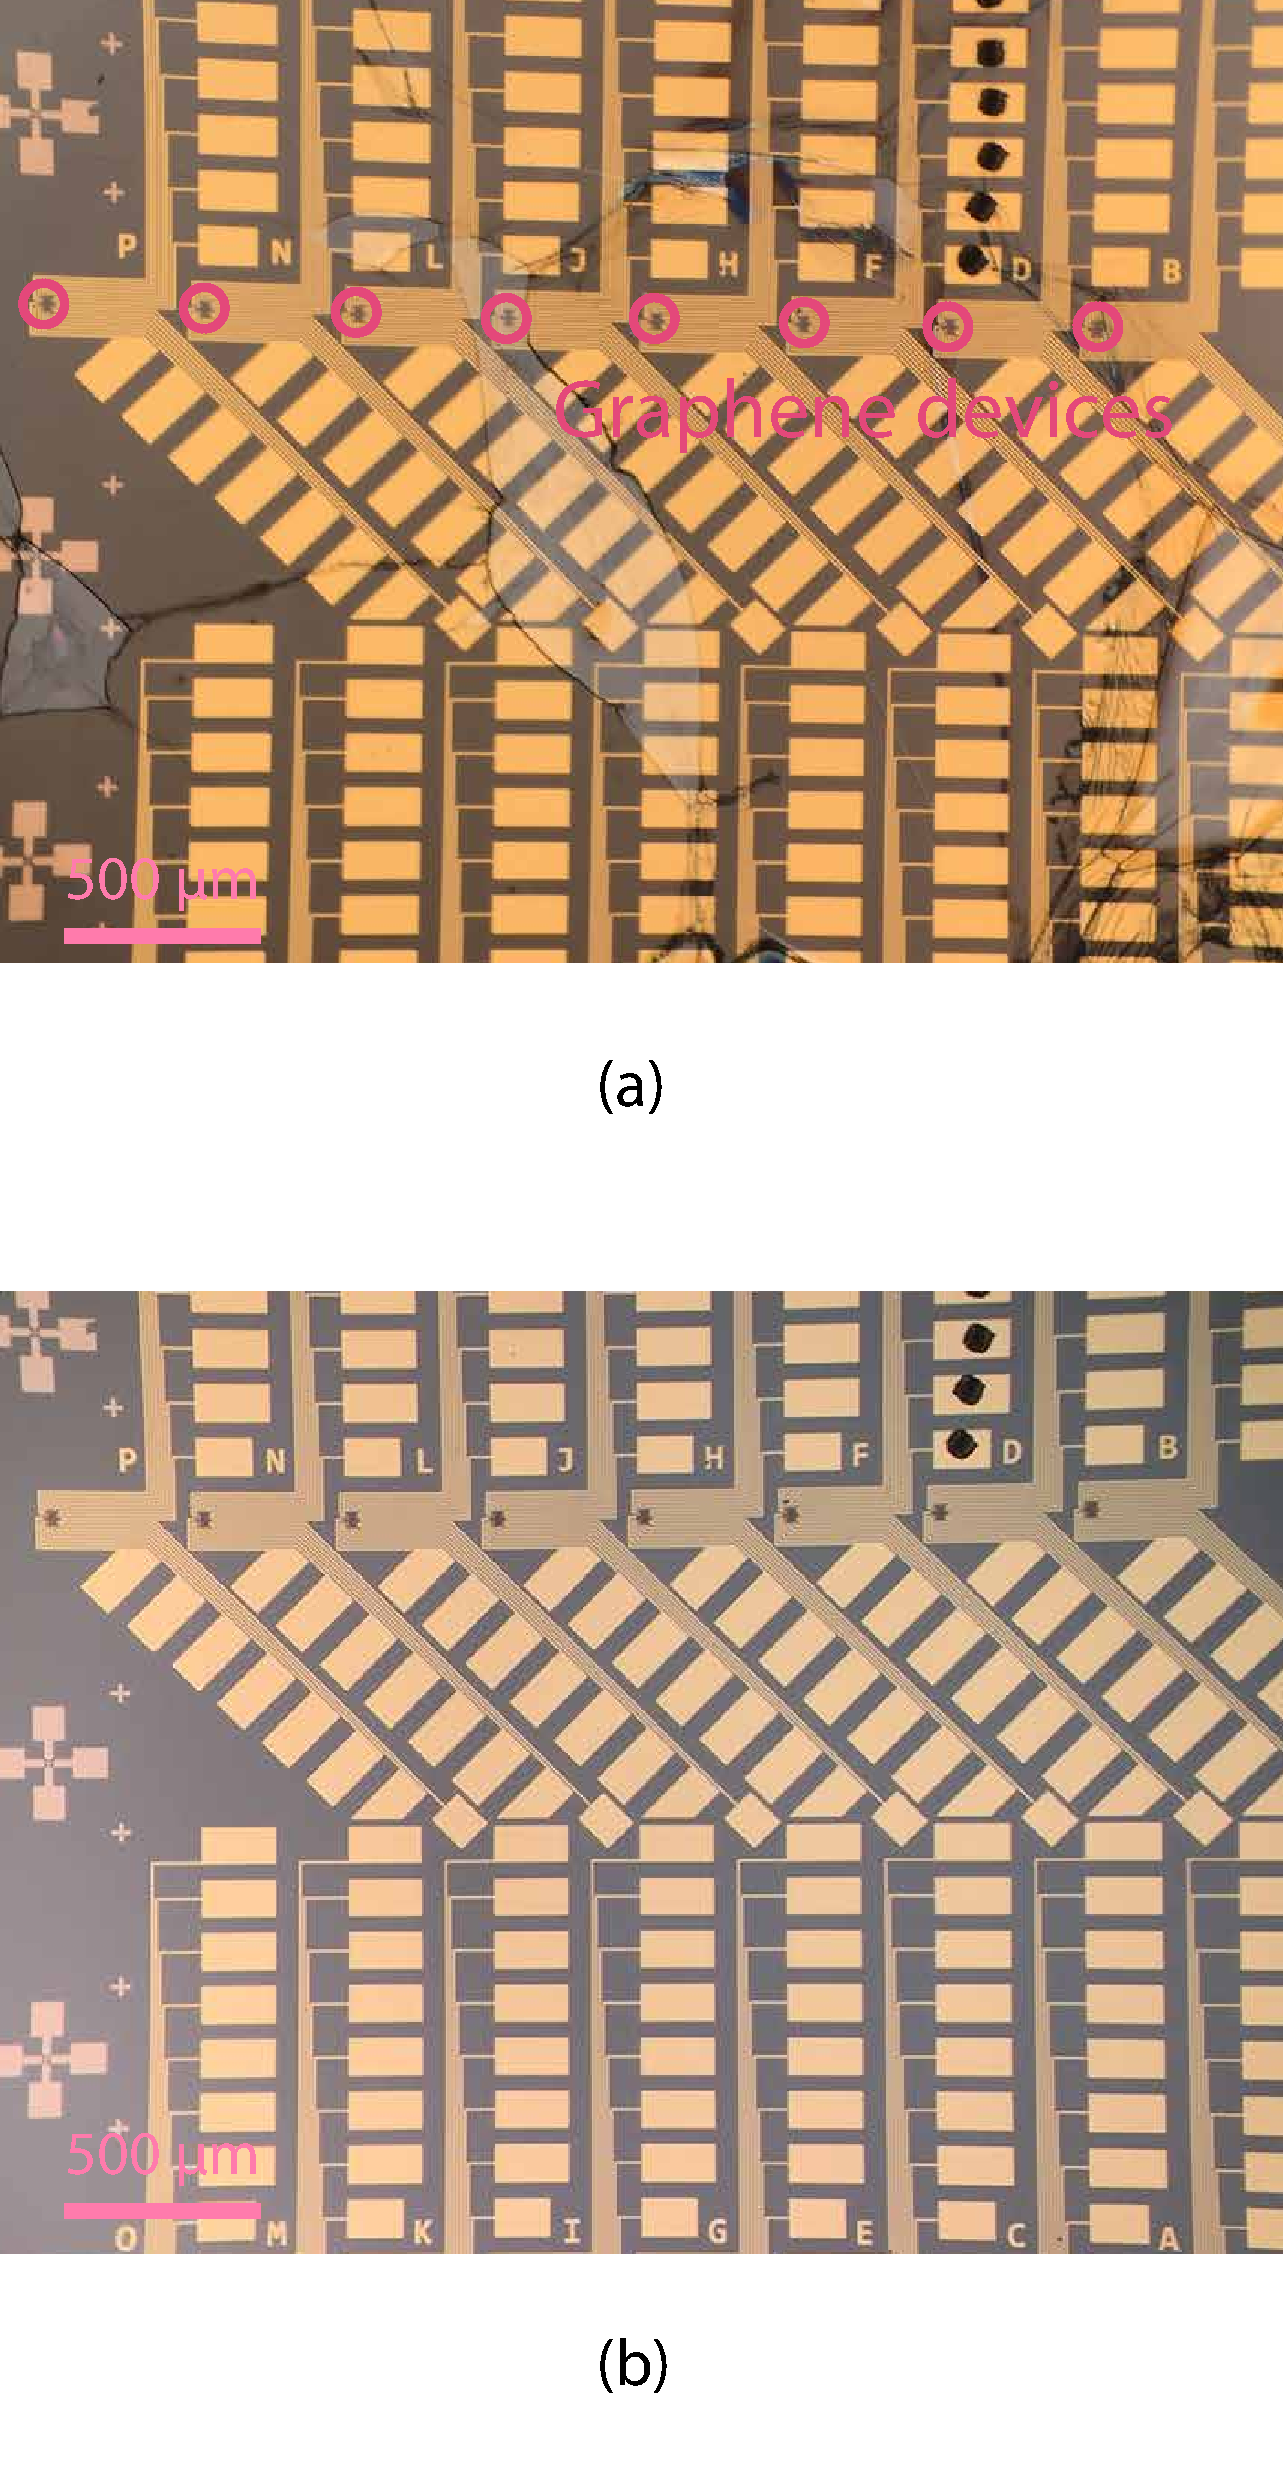
\includegraphics[width=.55\textwidth]{Drawing/SampleContaminant.pdf}
	\caption{Contaminants can be introduced by wet transfer. The source can be photoresist, copper etchant, or liquid trapped in the bubble formed from transferring. (a) Contaminants can be seen after graphene transfer. Only the graphene inside the red circles (zoomed-in image in Figure \ref{FIG:RIEBeforeEtching}) need to be protected with photoresist, and rest of the graphene can be removed along with the contaminants by RIE procedure. (b) Sample surface is clean after RIE procedure.}
	\label{FIG:SampleContaminant}
\end{figure}

\begin{figure}[h!]
	\centering
	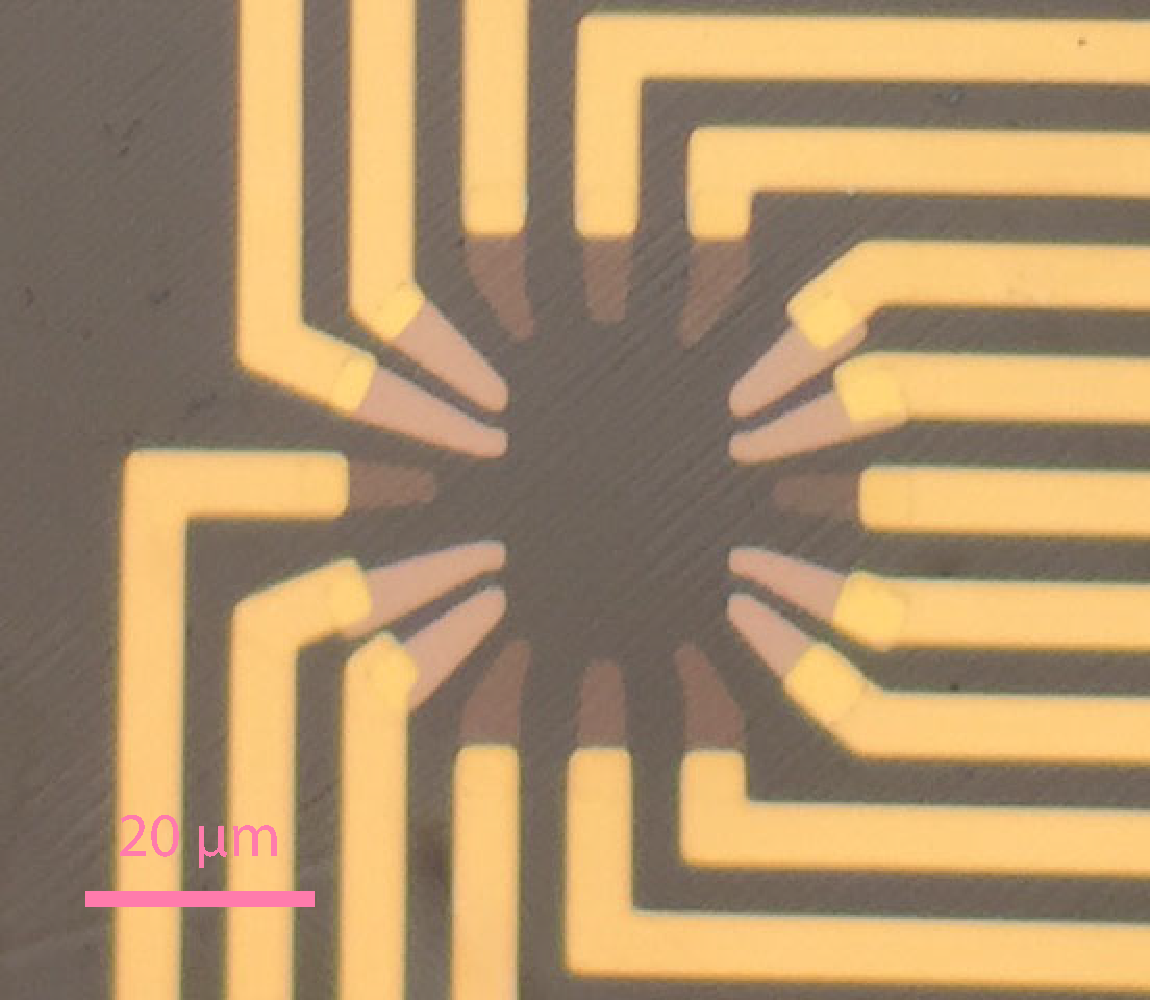
\includegraphics[width=.5\textwidth]{Drawing/RIEBeforeEtching.pdf}
	\caption{The graphene area of interest on pre-patterned LAO/STO sample. The patterns are for graphene and LAO/STO interface contact.}
	\label{FIG:RIEBeforeEtching}
\end{figure}

\subsubsection{One-step etching}

Before 2018 I was using the the one-step etching method (as shown in Figure \ref{FIG:HyflonTransfer}), that is to etch the graphene and clean the contaminants with RIE in one step. Figure \ref{FIG:SampleContaminant} shows the image of a sample before and after the RIE etching. In Figure \ref{FIG:SampleContaminant}(a), it can be seen that bubbles or foldings introduced from the wet transfer covers the entire sample. Fortunately in my experiments, most of the graphene transferred on LAO/STO needs to be etched away, and only the graphene device inside red circles in Figure \ref{FIG:SampleContaminant}(a) need to be covered with graphene. A zoomed-in image is shown in Figure \ref{FIG:RIEBeforeEtching}, with graphene covered with Hyflon. The metal patterns are contact electrodes for graphene and LAO/STO interface. Wrinkles on graphene can be seen, which are following the corrugations on the copper substrate during CVD growth. The patterns for the entire sample are designed in the way that there can be as many graphene devices fit in the sample as possible, so that there are higher chances of finding a clean graphene device. The contaminants are etched away with an aggressive RIE procedure (listed in Table \ref{TAB:RIESingleStep}). 

\begin{table}
	\centering
	\begin{tabular}{l|c}
		\hline
		Instrument	& RIE \\ \hline
		Gas	&	Oxygen \\ 
		Flow rate	&	19 sccm	\\ 
		Power & 50 W \\
		Pressure	&	300 mTorr	\\
		Time	&	60 - 180 s \\ \hline
	\end{tabular}
	\caption{One-step RIE etching recipe.}
	\label{TAB:RIESingleStep}
\end{table}

%\begin{figure}[h!]
%	\centering
%	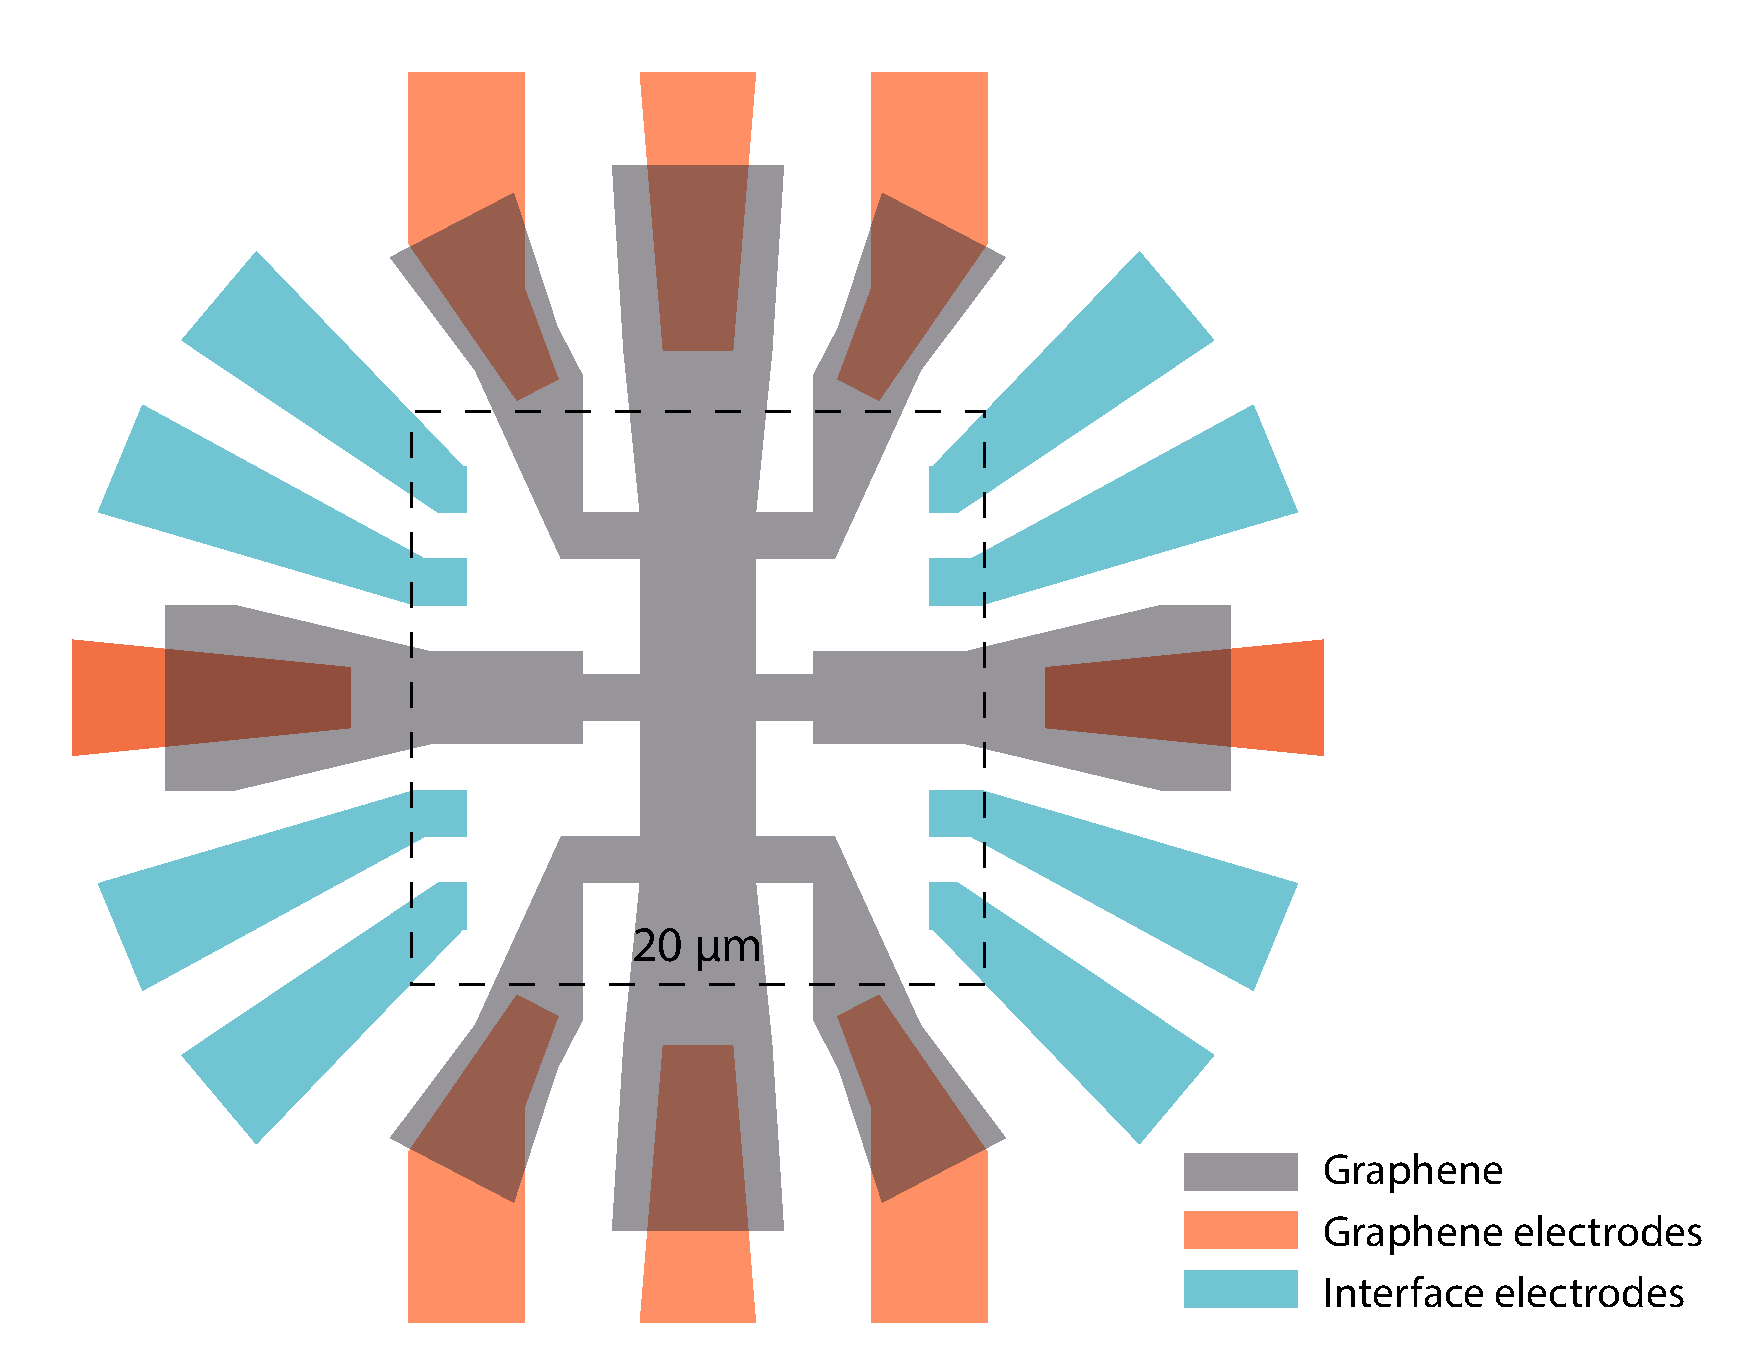
\includegraphics[width=.60\textwidth]{Drawing/GCOCanvas.pdf}
%	\caption{Graphene is shaped into Hall bars by RIE. Outside the Hall bar region, nanostructures need to be created inside the square region, on the interface of LAO/STO. Aggressive RIE process can damage the LAO/STO interface.}
%	\label{FIG:GCOCanvas}
%\end{figure}

As shown in Figure \ref{FIG:SampleContaminant}(b), the single-step RIE etching can completely clean the contaminants on LAO/STO. However, the etching can be problematic for the LAO/STO interface. As shown previously in Figure \ref{FIG:GCO}, the graphene Hall bar locates inside the 20 $\mu$m canvas area. When the graphene outside the Hall bar and surface contaminants are etched with the same aggressive RIE recipe, the bombardment would damage the LAO/STO interface and it would be impossible to write nanowires with c-AFM in some cases. However if I etch the sample with a milder recipe, the contaminants cannot be fully cleaned in some cases. 

\subsubsection{Two-step etching}

\begin{figure}[p]
	\centering
	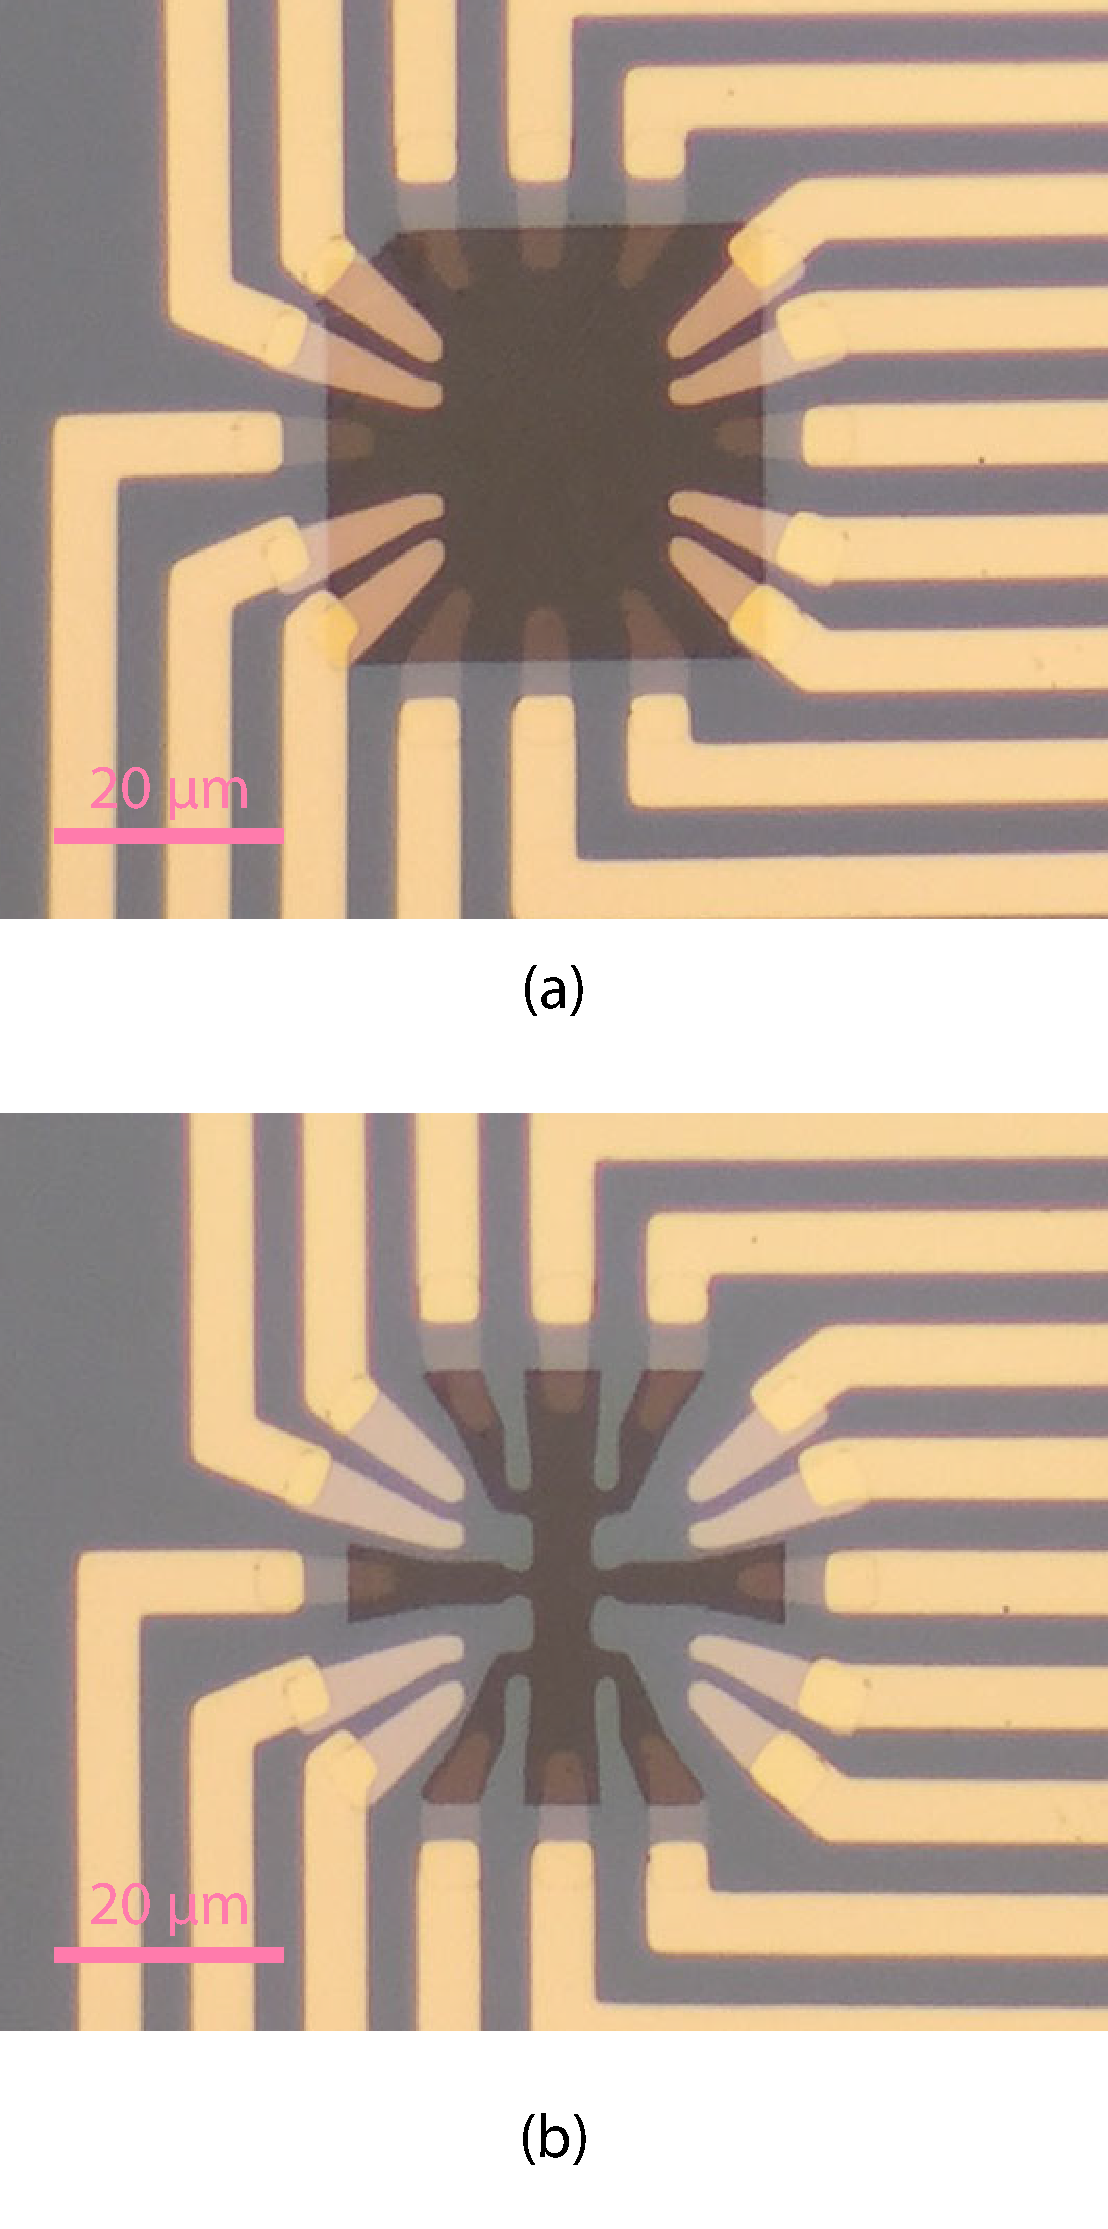
\includegraphics[width=.5\textwidth]{Drawing/RIETwoStep.pdf}
	\caption{Two-step graphene etching. (a) A square shape region is protected by AZ4210 photoresist. Outside of the square region the sample is etched with an aggressive RIE process to remove the contaminants introduced by wet-transfer. The figure shows the graphene with Hyflon. Photoresist has been washed off. (b) A second step of photolithography is performed and a Hall-bar shape region is protected by AZ4110 photoresist. Outside of the Hall-bar the Hyflon and graphene is etched away with a mild oxygen plasma barrel etching recipe, and the LAO/STO interface is still writable. The figure shows the graphene Hall-bar covered with Hyflon. }
	\label{FIG:RIETwoStep}
\end{figure}

To address the interface-damaging issue, I started to use the two-step etching method. The basic idea is to separate sample cleaning and graphene etching steps. As shown in Figure \ref{FIG:RIETwoStep}. In the first step of etching, the Hyflon and graphene are protected by photoresist in a square shape, that covers the Hall bar devices to be pattern in the next step and the LAO/STO canvas region. The rest of the sample is etch with an aggressive RIE step so that the contaminants on bonding pads and connection patterns are fully removed. After the etching the photoresist is washed away with acetone and IPA. In the second step, another layer of photoresist is spin-coated, and patterned into graphene Hall-bar device shape. Then the graphene and Hyflon outside the Hall bar region but covering the LAO/STO canvas are etched away with a much weaker oxygen plasma, so that the LAO/STO interface will not be damaged.

\begin{figure}[p]
	\centering
	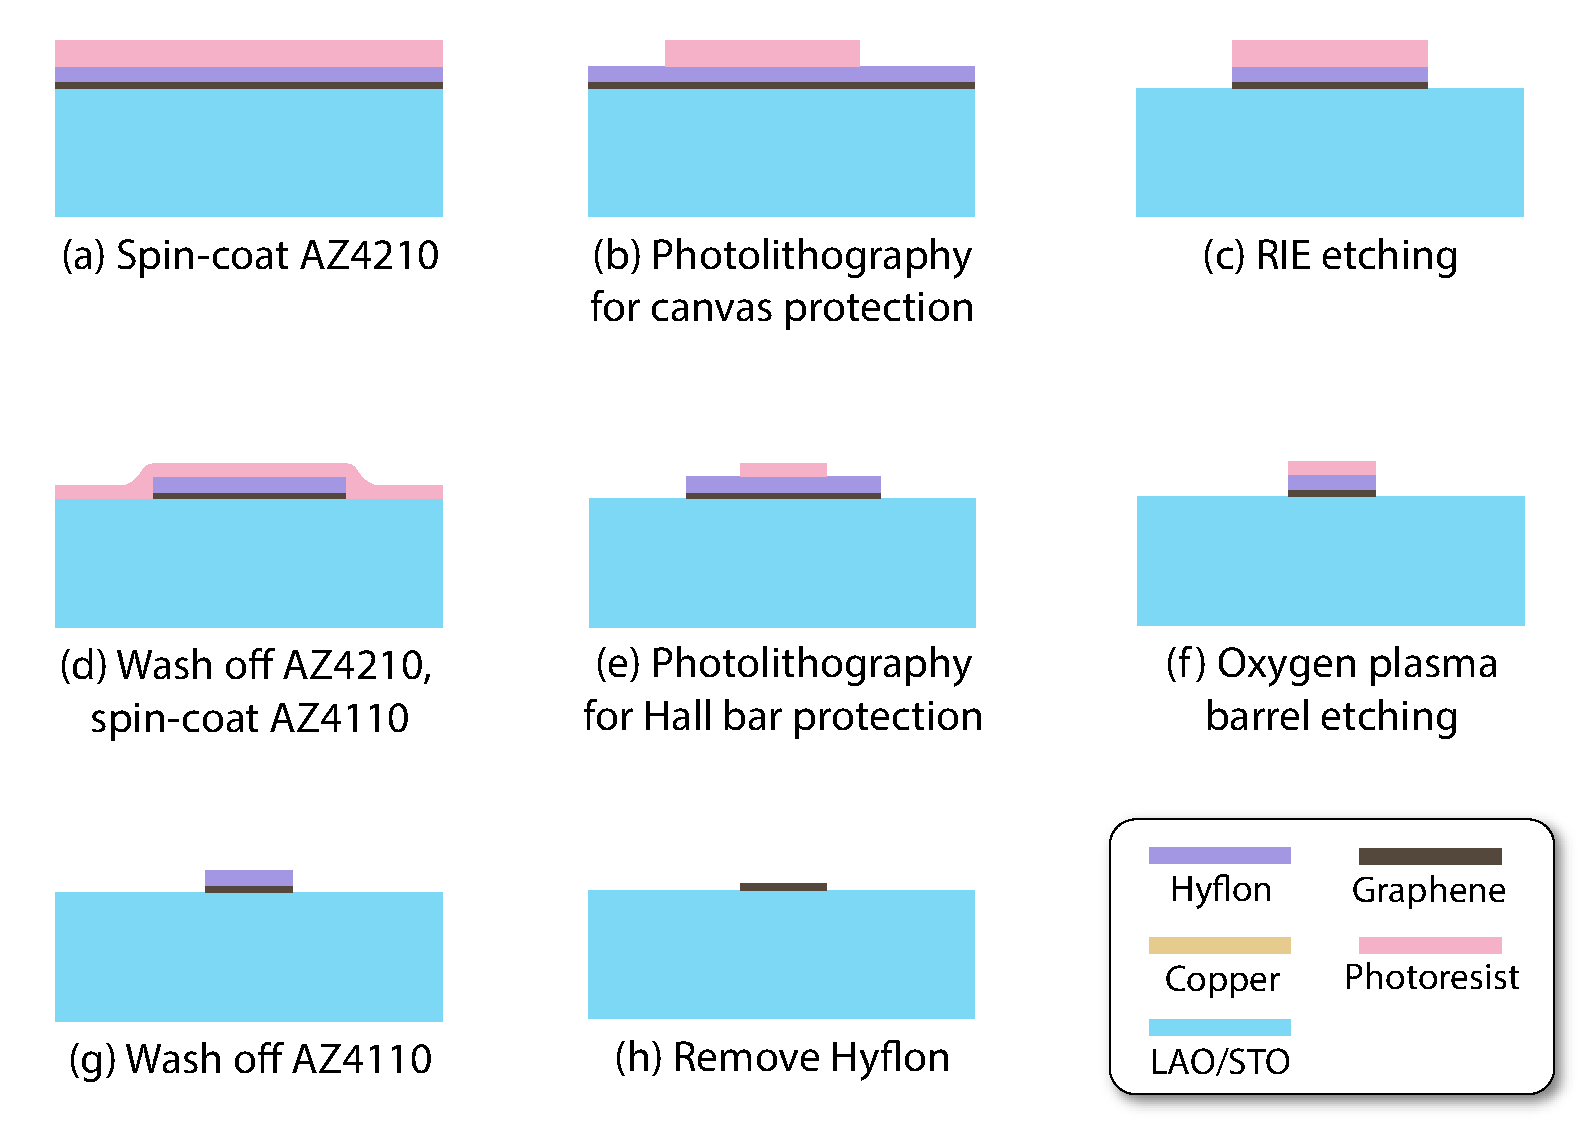
\includegraphics[width=1\textwidth]{Drawing/TwoStepEtching.pdf}
	\caption{Two-step graphene etching. (a) AZ4210 is spin-coated on Hyflon. (b) The photoresist is patterned into square-shape protection layer for the canvas. (c) An aggressive RIE process is used to fully remove the contaminants outside the canvas. (a) to (c) might be repeated if necessary. (d) AZ4110 is spin-coated. (e) Hall bar shape is patterned, to protect the Hyflon and graphene on the regions of interest. (f) A weak oxygen plasma etching step is used to remove the unwanted Hyflon and graphene. (g) AZ110 is washed of by solvents. (h) Hyflon is removed by FC-40.}
	\label{FIG:TwoStepEtching}
\end{figure}

The detailed procedures are shown in Figure \ref{FIG:TwoStepEtching}. Right after graphene is transferred onto LAO/STO and the supporting photoresist is washed off, it is spin-coated with AZ4210. The square-shape is patterned with photolithography to protect the canvas. Then the sample is etched with RIE, until all the contaminants are cleaned. In some cases, the contaminants needs long etching time, and photoresist may be etched through. Multiple photolithography and RIE etching steps will be needed. For the same reason, AZ4210 (2.1$\mu$m thick) is preferred than AZ4110 (1.1 $\mu$m thick). After that, AZ4210 is washed off, and AZ4110 is spin-coated. Photolithography on AZ4110 has higher precision. One thing I noticed was that the developing time required for AZ4110 is much longer than usual, possibly because the previous RIE etching changed the surface hydrophilicity and make the exposed photoresist harder to be washed off. After the Hall bar is patterned with inverse pattern, the sample is etched with a weak oxygen plasma barrel etching recipe, and shape the graphene and Hyflon into Hall bars (Figure \ref{FIG:RIETwoStep}). The recipe for photolithography and etching are listed in Table \ref{TAB:TwoStepPL} and Table \ref{TAB:TwoStepEtching}.


\begin{table}
	\centering
	\begin{tabular}{l|cc}
		\hline
		Photoresist	& AZ4210 (step 1) & AZ4110 (step 2) \\ \hline
		Spin-coating	&	4000 rpm	&	4000 rpm \\ 
		Baking	&	95 $^{\circ}$C	&	95 $^{\circ}$C	\\ 
		UV dose	&	170 mJ	&	100-120 mJ	\\
		Developer : DI-water	&	1 : 4 &	1 : 4 \\ 
		Developing time	&	120 s	&	240 - 600 s \\
		\hline
	\end{tabular}
	\caption{Two-step etching photolithography recipe. First layer of AZ4210 is used to protect the canvas against the aggressive RIE for contamination removal. Second layer of AZ4110 is for graphene Hall bar protection, and only need to resist mild oxygen plasma etching.}
	\label{TAB:TwoStepPL}
\end{table}

\begin{table}
	\centering
	\begin{tabular}{l|cc}
		\hline
		Instrument	& RIE (step 1)	&	Barrel etcher (step 2) \\ \hline
		Gas	&	Oxygen &	Oxygen \\ 
		Pressure	&	300 mTorr	&	$\sim$ 600 mTorr \\
		Power	&	50 W	&	100 W \\
		Time	&	200 - 400 s &	300 s\\ \hline
	\end{tabular}
	\caption{Two-step etching recipe. Although it seems that the barrel etcher is running at higher power, the structure of the instrument make the etching much less invasive compared to RIE.}
	\label{TAB:TwoStepEtching}
\end{table}

\subsection{Hyflon removal}

Over the entire processing, the graphene is covered with Hyflon until the last step. The Hyflon is only solvable in perfluorinated solvent such as FC-40. On one hand, this makes it possible for Hyflon to serve as a protection layer for all the other chemicals like acetone, IPA or photoresists. On the other hand, it also make Hyflon hard to be fully removed. I used two recipe for Hyflon removal. 

\subsubsection{High temperature method} FC-40 heated up to 165 $^{\circ}$C in a beaker. The boiling point of FC-40 is about 175 $^{\circ}$C and it decomposes into HF, therefore I keep the temperature lower than that. Once the sample is placed in FC-40, the beaker is taken off the hot place and left on a shaking stage at 100 rpm, and the sample is shaken in FC-40 for 12 hours while it cools down to room temperature. Then the sample is taken out and dried with nitrogen.

\subsubsection{Low temperature method} FC-40 is heated up to 70 $^{\circ}$C in a beaker. After the sample is immersed in FC-40, the beaker is shaken at 100 rpm while the temperature is kept at 70 $^{\circ}$C for 12 - 24 hours. Then the sample is taken out and dried with nitrogen. I started to use this method since 2017.
\\

It is hard to determine which method is more preferable. The room temperature method does seem to be less harsh, and might affect the graphene and LAO/STO. However, the residue on graphene is more than the high temperature method. There was a period of time (about a year) when I could not produce high quality graphene/LAO/STO sample. Whether or not it is related to switching from the high temperature method to low temperature method for Hyflon removal is still uncertain.

\subsection{AFM cleaning of graphene}

From the past experiences, all the solvents including DI-water, IPA and FC-40 would leave a layer of nano-particles on sample surface, until cleaned by oxygen plasma. For graphene/LAO/STO sample, even a weak recipe of oxygen plasma etching can potentially cause structural damage to the graphene. Therefore, the nano-particles from solvents, especially FC-40, and the residues of Hyflon are cleaned with AFM contact mode scanning, as a final step of processing. 

\begin{figure}[p]
	\centering
	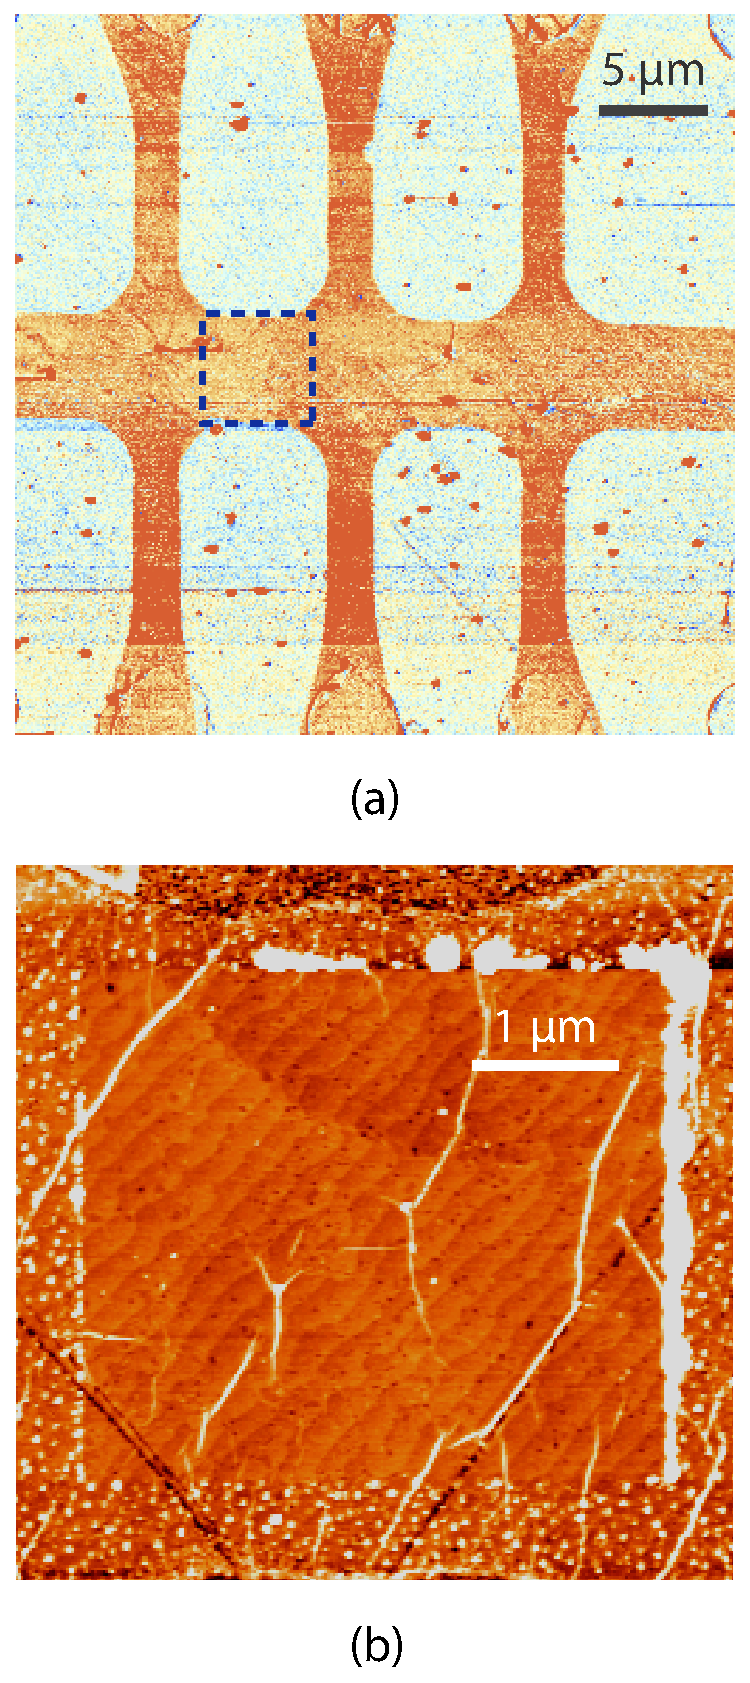
\includegraphics[width=0.4\textwidth]{Drawing/GrapheneAC.pdf}
	\caption{AFM cleaning of graphene. (a) The organ Hall bar region is the graphene, after Hyflon removal in FC-40. Particles on graphene can be observed. (b) Zoomed-in image of the square region in (a). The center has been scanned in AFM contact mode. Particles are pushed to the top and right edges. Terraces of LAO/STO and wrinkles can be observed.}
	\label{FIG:GrapheneAC}
\end{figure}

Figure \ref{FIG:GrapheneAC} shows the AFM images of graphene before and after cleaning. Figure \ref{FIG:GrapheneAC}(a) is the AFM AC mode phase image. The Hall bar shape in orange is the graphene, and the LAO surface is in cyan. As can be seen, particles of different sizes can be observed. Larger particles ($\sim$ 100 nm) are probably from the the FC-40, while the smaller particles (< 100 nm) are the residues of Hyflon. Figure \ref{FIG:GrapheneAC}(b) is the zoomed-im image of the squared region in \ref{FIG:GrapheneAC}(a), after the center is been scanned with AFM in contact mode. Particles are pushed to the edges of the square, and it can be seen that the scanning is bottom to up, left to right. Inside the clean region, terraces ($h = 4 \mathrm{\AA}$) of the LAO/STO substrate can also be observed. Wrinkles of the graphene are formed during the transfer or AFM contact scan process. Mechanical strength of graphene is high enough\cite{} to withstand the contact scanning, however it is possible that graphene is broken by the AFM tip, especially when the raster scan speed is too fast and large amount of resilient contaminants are present on graphene (and a large contact force has to be applied), or when the AFM tip is scanning from the LAO to graphene from the edge with a large contact force. Typical cleaning recipes with on models of AFM are listed in Table \ref{TAB:AFMCleaning}, with which the graphene does not break.
\\

\begin{table}[h!]
	\centering
	\begin{tabular}{l|cc}
		\hline
		AFM model	&	Asylum MFP3D	&	Asylum Cypher \\ \hline
		Tip spring constant	&	3 N/m	& 3 N/m	\\ 
		Deflection set-point	&	$0.05 - 0.5$ V	&	$0.1 - 1.0$ V	\\		
		Contact force	&	$40 - 400$ nN	&	$20 - 200$ nN	\\
		Scanning speed	&	10 $\mu$m/s	&	10 $\mu$m/s \\ 
		Line separation	&	$10 - 20$ nm	&	$10 - 20$ nm	\\ \hline
	\end{tabular}
	\caption{Graphene cleaning recipes on Asylum MFP3D and Cypher.}
	\label{TAB:AFMCleaning}
	
\end{table}

To prove that the sample is clean after AFM cleaning, an room temperature STM measurement is performed. Tunneling currents are measured from graphene surface to a tungsten tip. From the AFM image the graphene atoms can be identified, which proves that the graphene on LAO/STO is atomically clean. 
\\

\begin{figure}[h!]
	\centering
	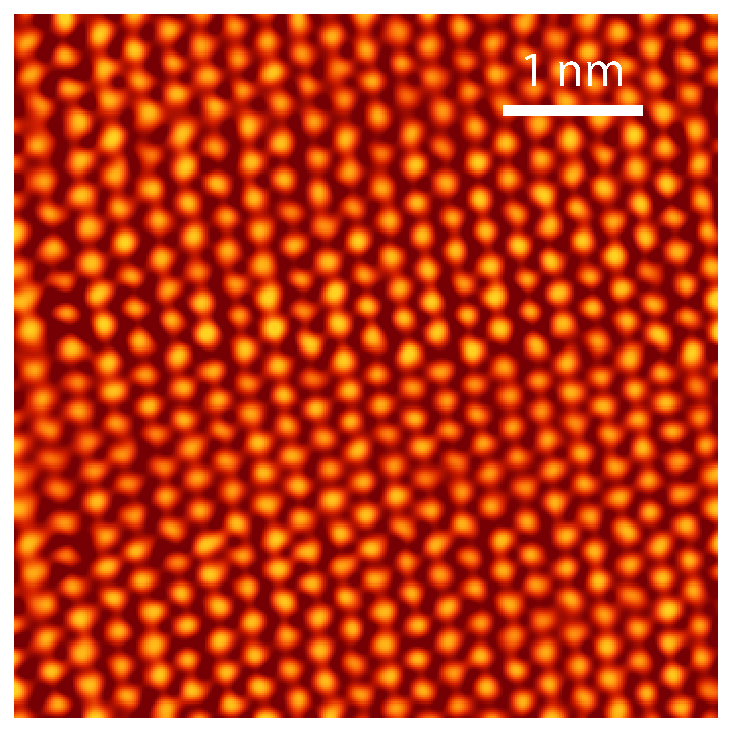
\includegraphics[width=0.45\textwidth]{Drawing/GrapheneSTM.pdf}
	\caption{STM image of graphene on LAO/STO after AFM cleaning.}
	\label{FIG:GrapheneSTM}
\end{figure}

%\subsection{Graphene cutting with nanoscale anode oxidation}

%Another approach of shaping graphene into devices is to directly etch it with c-AFM.  

\subsection{Graphene/LAO/STO nano-scale device lithography}

The experiments on graphene, such as Klein tunneling\cite{allain2011klein, katsnelson2006chiral, young2009quantum, shytov2008klein}, edge state mixing\cite{williams2007quantum, abanin2007quantized, lohmann2009four, amet2014selective}, band structure engineering using superlattice\cite{forsythe2018band}, rely on the Dirac cone band structure and tunability of carriers from electrons to holes. The ability to control the charge neutrality point is central to controlling these exotic properties of graphene. c-AFM writing is proved to be a powerful tool to create nanostructures on LAO/STO interfaces. Pattern nano-scale devices on graphene/LAO/STO reversibly with c-AFM is one of the major techniques I have been trying to develop in my research. 

\subsection{c-AFM lithography and PFM imaging}
\begin{figure}[p]
	\centering
	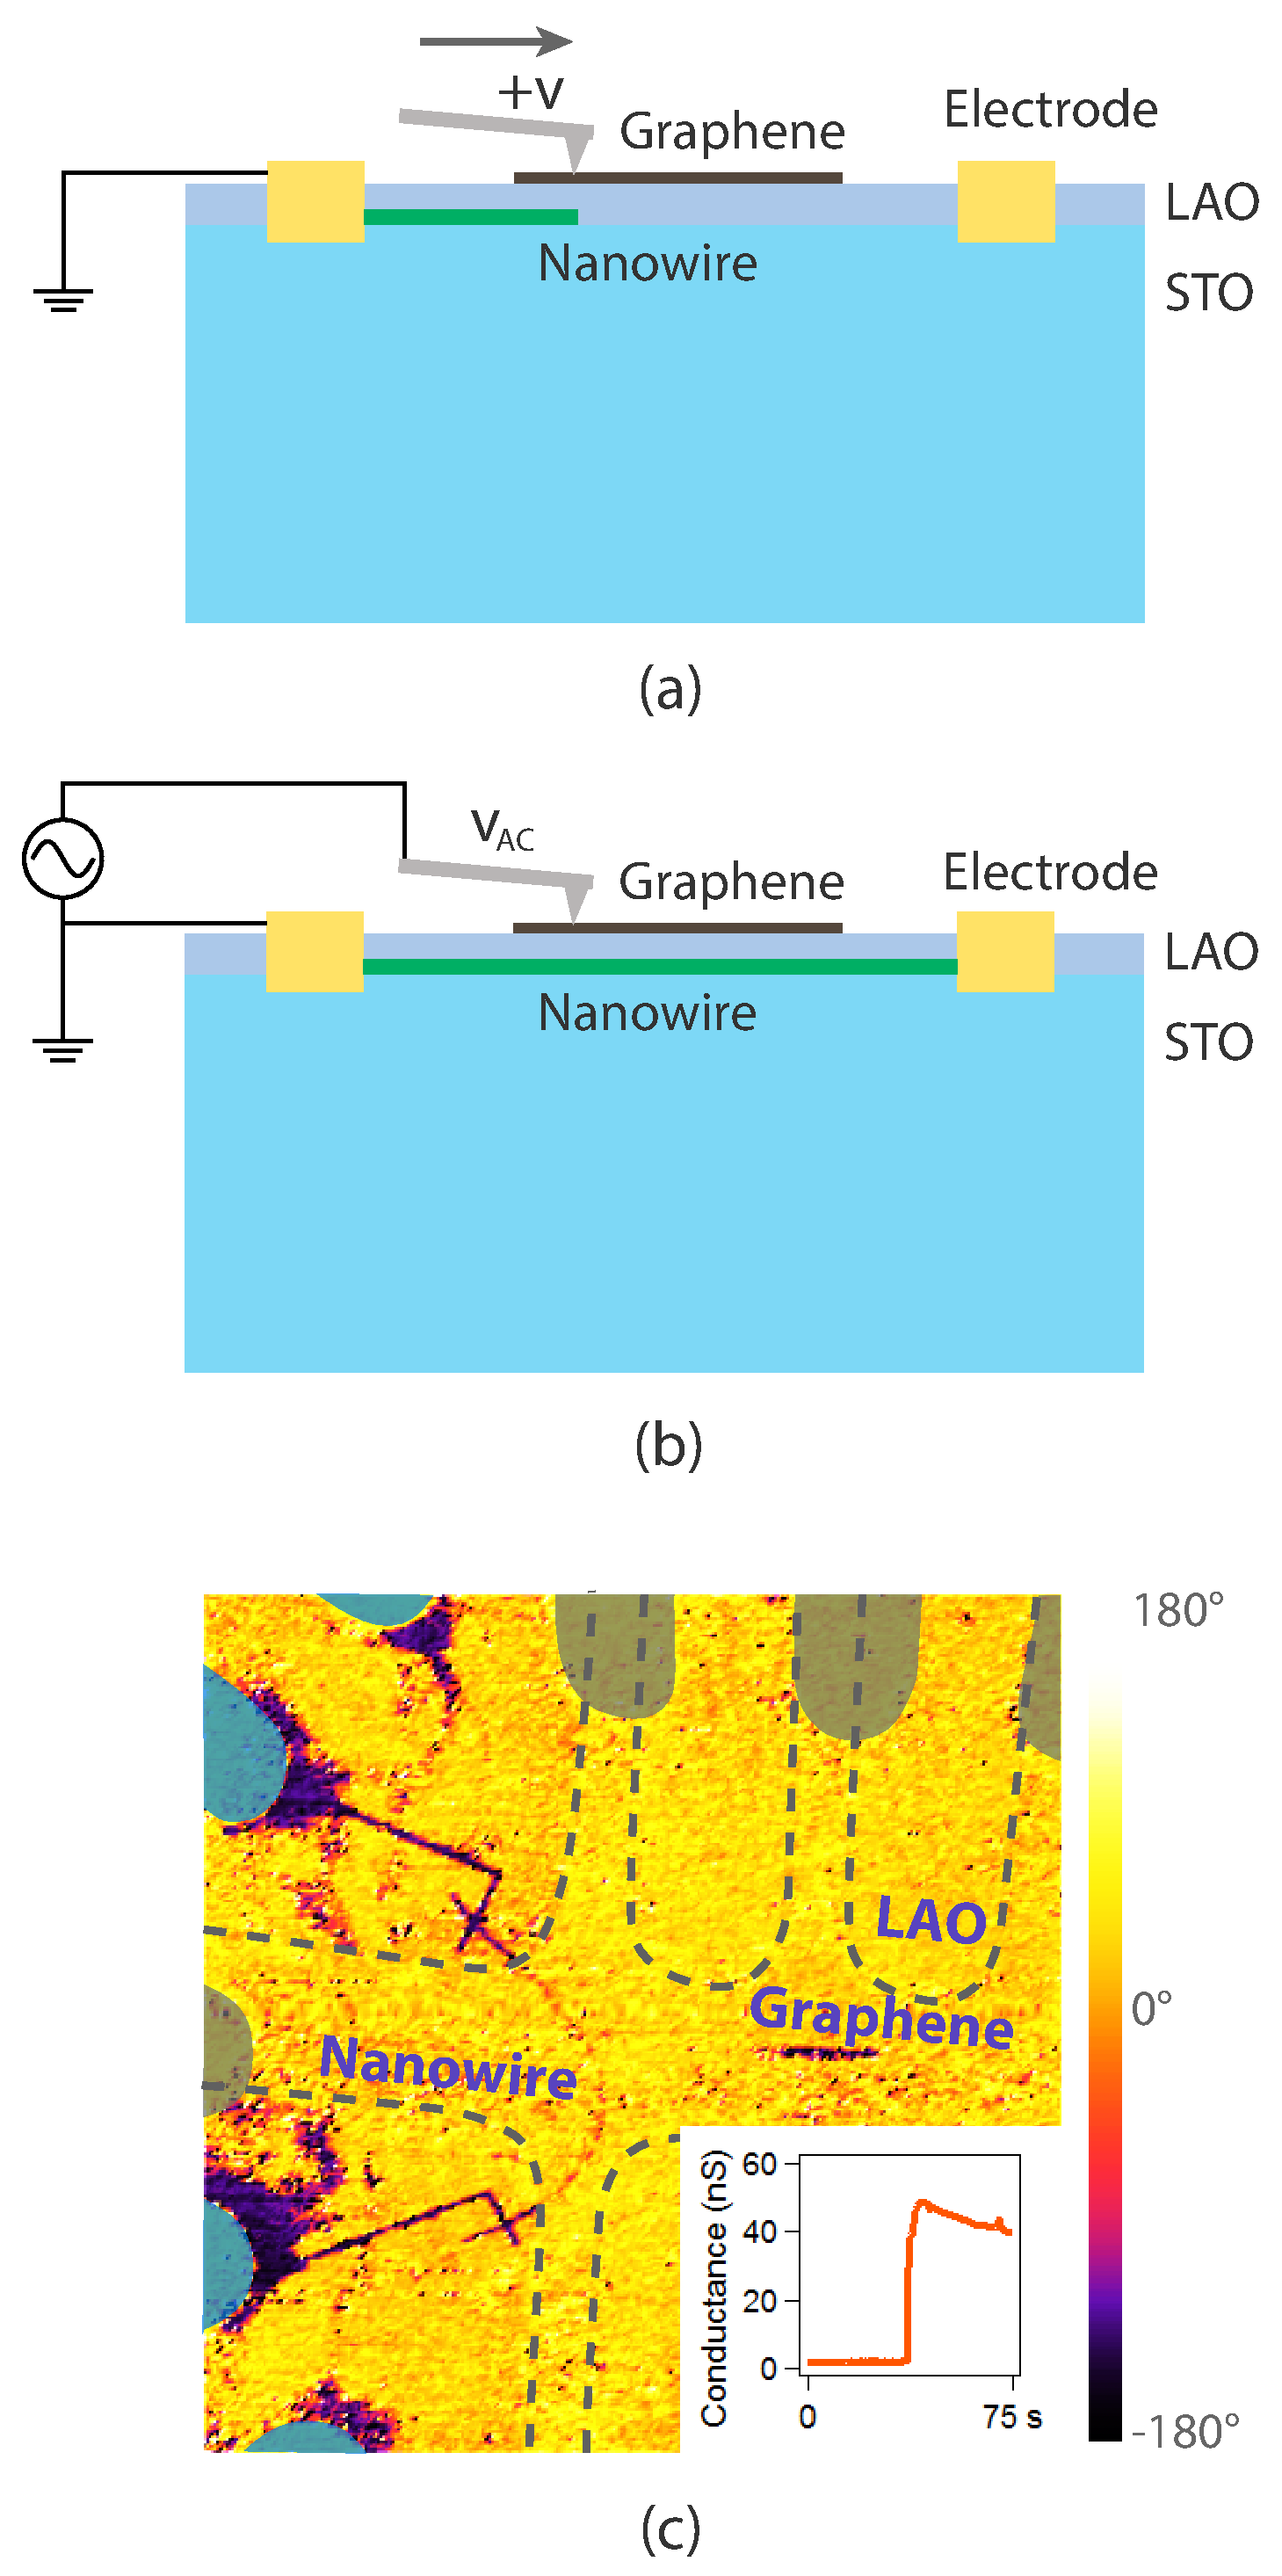
\includegraphics[width=0.6\textwidth]{Drawing/GraphenePFM.pdf}
	\caption{(a) c-AFM lithography of graphene/LAO/STO nanowire. (b) PFM measurement setup. (c) PFM image of the nanowire on LAO/STO interface, underneath the graphene. The inset shows the sudden jump of conductance after the two interface electrodes are connected.}
	\label{FIG:GraphenePFM}
\end{figure}

Figure \ref{FIG:GraphenePFM} demonstrates the setup of c-AFM lithography on graphene/LAO/STO, and the subsequent PFM imaging of the nanowire underneath the graphene. The setup of c-AFM lithography is similar to bare LAO/STO samples. The interface electrodes is grounded or measure. A positive voltage $V_\mathrm{tip} > +6V$ is applied to the c-AFM tip, while the tip sketches between the two interface electrodes. A protective resistor of 1 G$\Omega$ is connected in series with the tip and voltage source (not shown in Figure \ref{FIG:GraphenePFM}). The graphene is disconnected and floating in this experiment. The tip goes through the graphene covered area before two interface electrodes are connected. The typical voltage applied to the AFM tip is $+15$ V, and the tip moving speed is 0.5 -- 1 $\mu$m/s, but can be as high as 10 $\mu$m/s in some cases. Contact force is about 20-80 nN. A sudden increase of conductance between two electrodes can be observed (inset of Figure \ref{FIG:GraphenePFM}(c)), indicates that a conductive channel has been created. 

A subsequent PFM measurement is performed. An AC voltage (with modulation frequency $f$ close to the PFM resonance frequency of the sample) is applied to the c-AFM tip, while the tip scans in contact with the sample. The alternating voltage from the tip modulates the carrier density on the LAO/STO interface, and the carrier density change will cause deformation of STO through the Jahn-Teller effect\cite{}. The area that previously written with nanowire would respond differently to the AC tip voltage, causes contrast on the PFM image. Figure \ref{FIG:GraphenePFM}(c) shows the PFM phase image of the nanowire written. The region colored in blue are the interface electrodes, and the region in gray are electrical contact with graphene. The graphene covered regions are enclosed with dashed lines. The narrow path in dark purple color is the nanowire previously written with c-AFM. The path under the graphene regions is dimmer than the outside sections, indicating the shielding effect of graphene against both the c-AFM lithography voltage and the PFM AC voltage on tip.


\subsection{More about the c-AFM writing conditions on graphene and damage thresholds}

The graphene on LAO/STO makes the c-AFM lithography more complicated than on bare LAO/STO. As discussed in Section \ref{SEC:AFMLitho}, the lithography and erasion of nanowire on the interface relies on the water-cycle and protonation induced by c-AFM tip voltage. It was also found that the surface conditions of LAO can affect the interface 2DEG\cite{}. Graphene on LAO also changes the critical thickness of LAO/STO\cite{aliaj2018probing}. 
\\

\begin{figure}[h!]
	\centering
	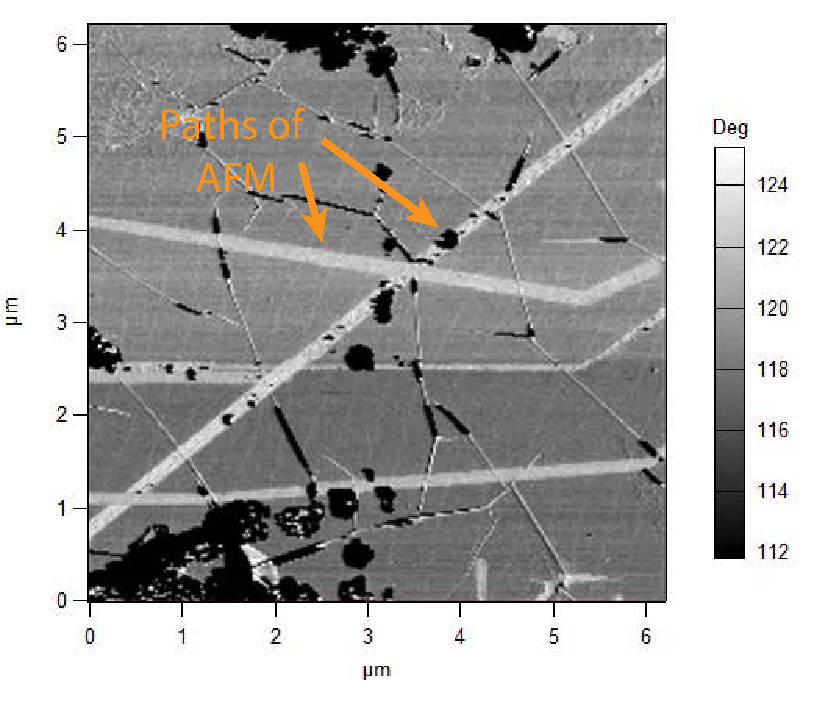
\includegraphics[width=.7\textwidth]{Drawing/GrapheneDamages.pdf}
	\caption{Damages on graphene from c-AFM lithography. On the AFM paths the graphene is oxidized and show contrast on the phase image.}
	\label{FIG:GrapheneDamages}
\end{figure}

The LAO/STO is fairly robust under the writing and erasing with c-AFM. The graphene however, can be damaged by a high negative voltage on the tip, from the anode oxidation effect\cite{}. It was reported\cite{} that the graphene damaging threshold voltage on the c-AFM is about $V{\mathrm{damage}} \approx 6 V$. This voltage is dependent on whether the graphene is floating or grounded and how much current is flowing between the tip and graphene. Figure \ref{FIG:GrapheneDamages} is an AC phase image of damaged graphene. The light color paths are from AFM sketching with $-15$ V on the tip, at 400 nm/s speed and 75 nN contact force. The contrast clearly shows the oxidation on graphene. The upper and lower regions of the graphene are electrically disconnected. To avoid oxidation damage to graphene, the tip voltage is limited to $-5$ V when the graphene is grounded, and $-8$ V when the graphene is floating while performing c-AFM on graphene with a negative voltage. From my experience the damaging thresholds are also related to the AFM tip condition or graphene surface roughness, but in general under these voltages the graphene damage can be avoided. The AFM lithography parameters are listed in Table \ref{TAB:GCOLithography}.

\begin{table}[h!]
	\centering
	\begin{tabular}{l|cc}
		\hline
				&	Writing	&	Erasing \\ \hline
		Tip spring constant	&	3 N/m	& 3 N/m	\\ 
		Deflection set-point	&	0.05 - 0.5 V	&	0.1 - 1.0 V	\\	
		Tip voltage	&	+10V to +20V	& -5V (graphene grounded) \\
			&	& to -8V (graphene floating) \\
		Contact force	&	80 nN	&	80 nN	\\
		Tip speed	&	0.4 - 10 $\mu$m/s	&	0.4 - 10 $\mu$m/s \\ 
	\end{tabular}
	\caption{c-AFM writing and erasing parameters on graphene/LAO/STO samples.}
	\label{TAB:GCOLithography}
	
\end{table}

\chapter{Graphene/LAO/STO heterostructure device}

This chapter is about the transport properties of graphene device on graphene/LAO/STO. It is also found that graphene can be reversibly doped with c-AFM lithography technique, similar to the nanostructure lithography on bare LAO/STO. Two experiments are discussed in details: edge-state mixing on graphene $p$-$n$ junctions and graphene superlattice patterning.

\section{Transport measurement in graphene}

The properties of graphene on LAO/STO is different from those on SiO$_2$ or hBN substrates due to the unique properties of the LAO/STO. This section will discuss the transport properties of graphene/LAO/STO samples. 

The geometry of the sample is illustrated in Figure \ref{FIG:HallDevice}. The graphene on LAO/STO is patterned into Hall bar shapes, with the procedure discussed in previous chapters. Gold electrodes make contact to the graphene from the surface of LAO. The bottom of the sample is pained with silver epoxy, and backgate voltage is applied to the bottom to control the global chemical potential of graphene. Current flows through the main channel of graphene, with a typical $I = 100$ nA. Longitudinal and transverse voltages are measured from the leads shown in Figure \ref{FIG:HallDevice}(b).

\begin{figure}[p]
	\centering
	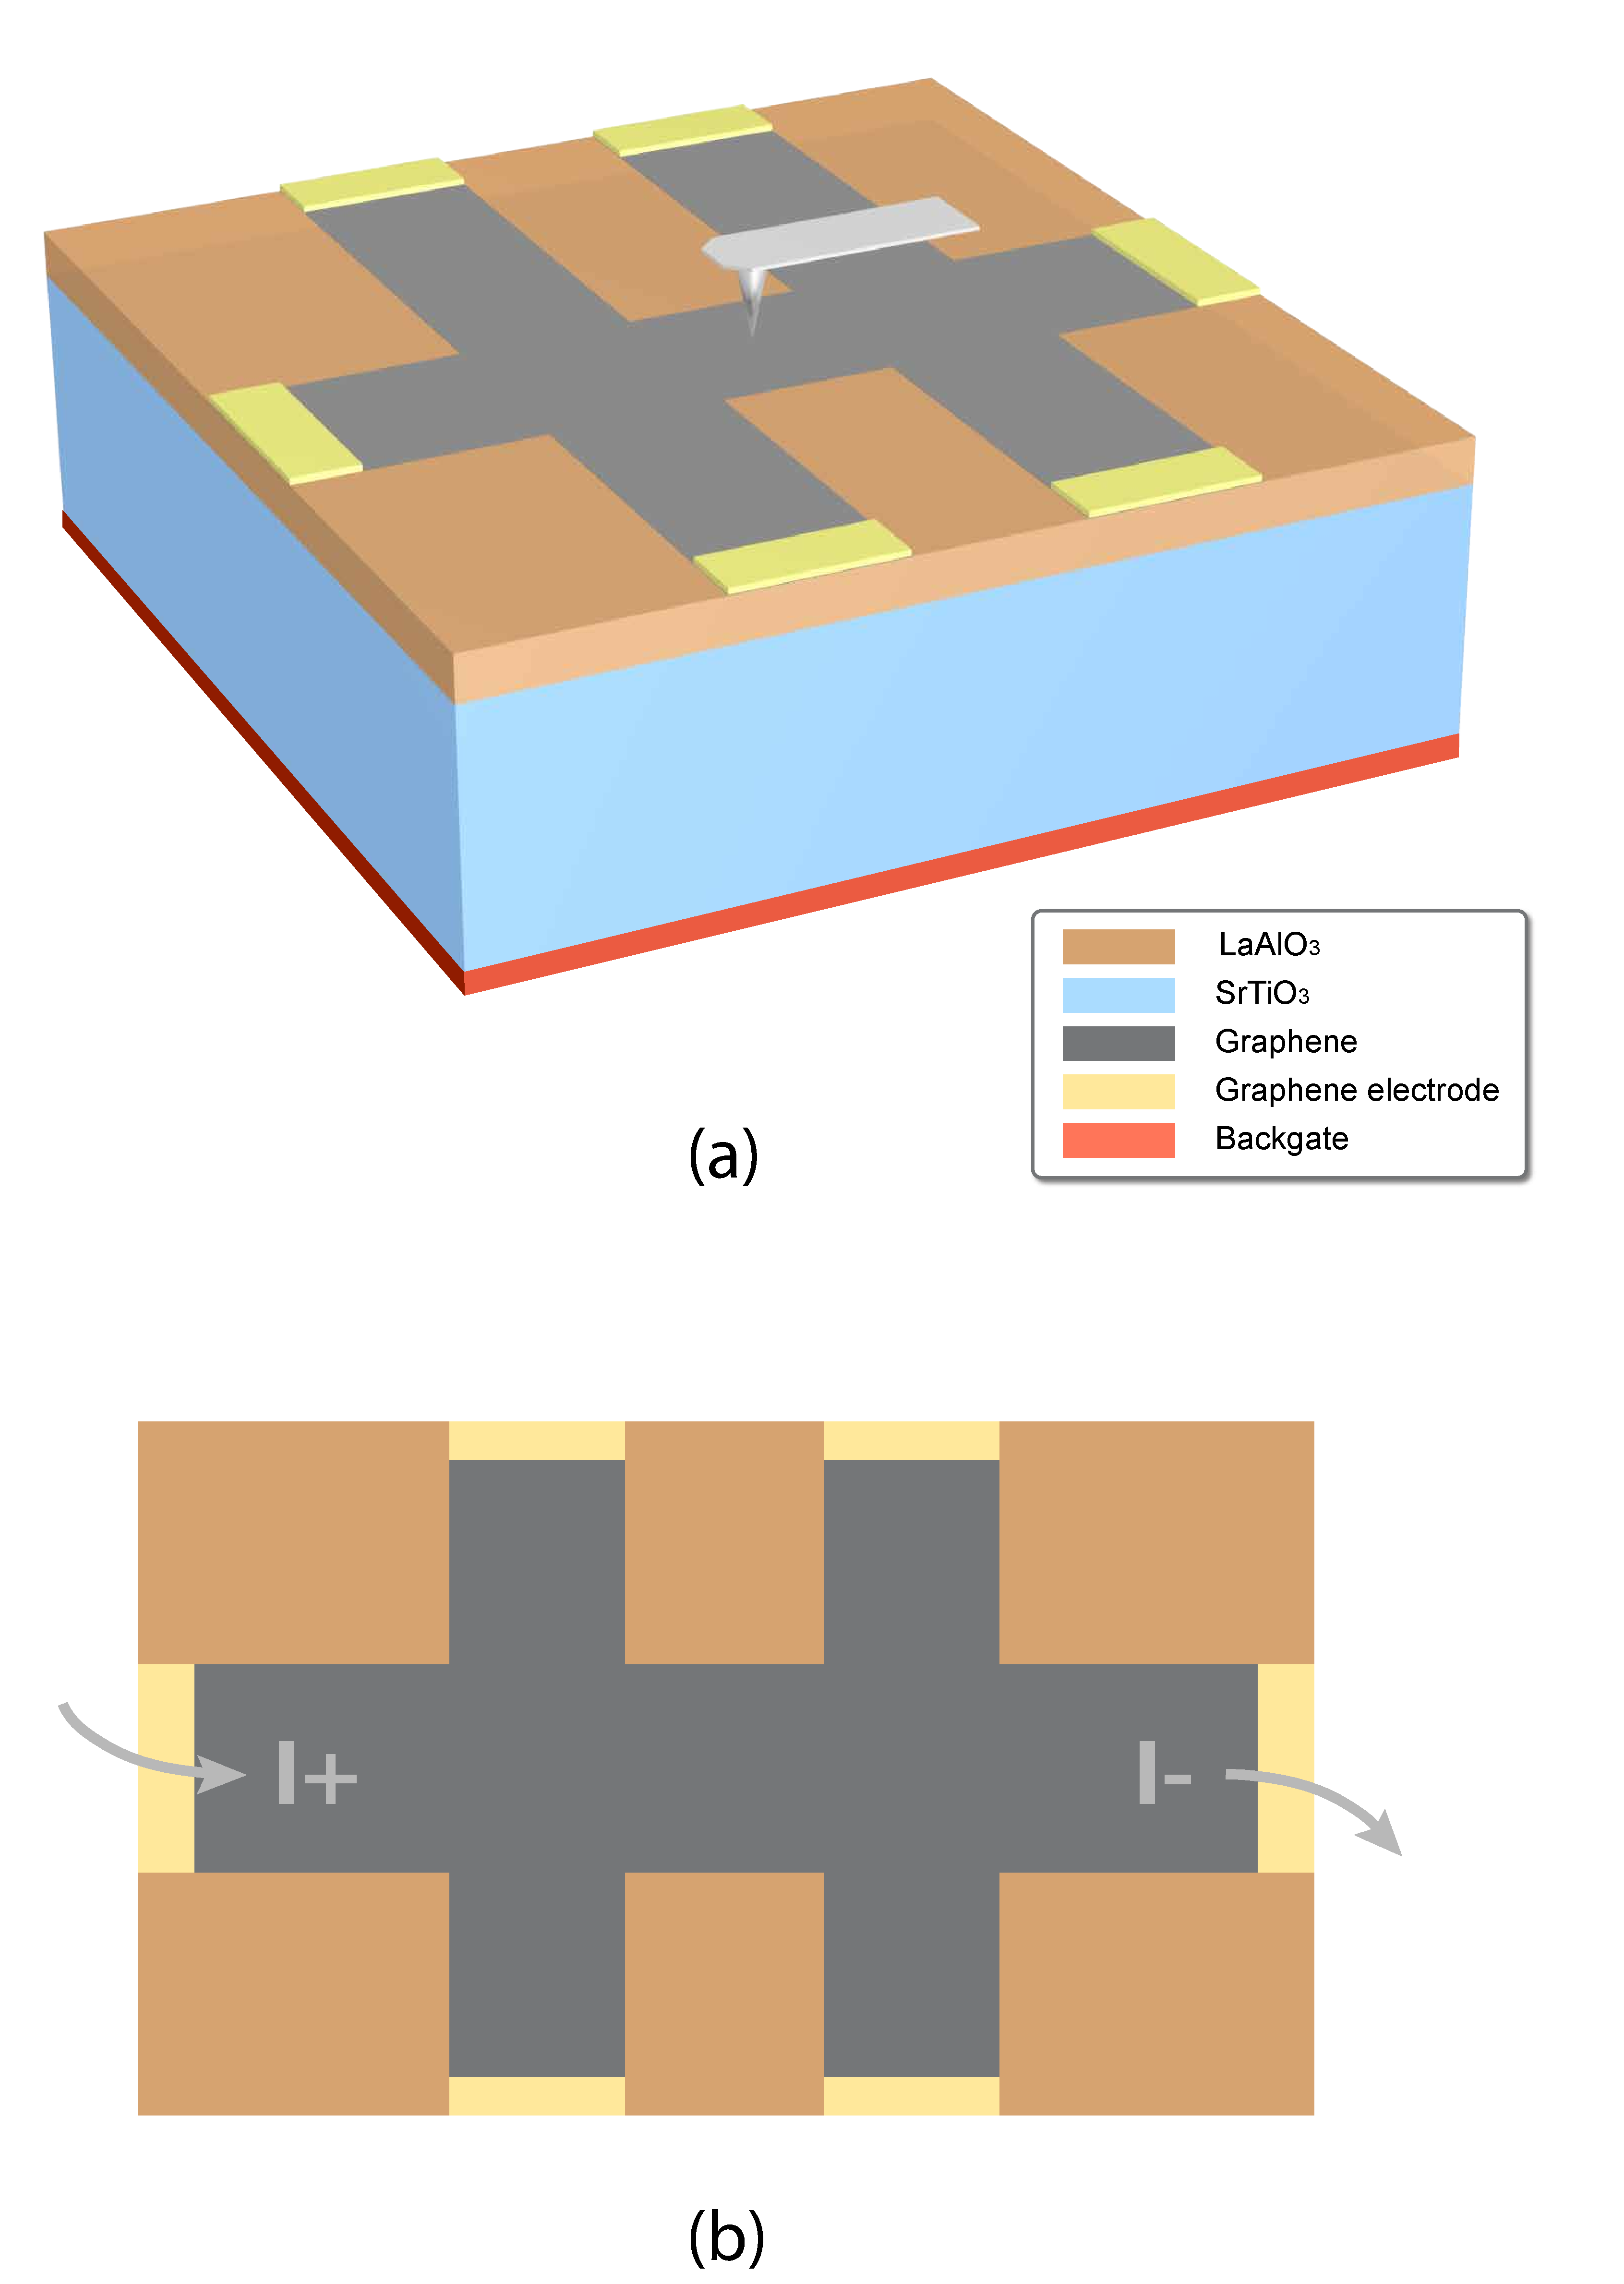
\includegraphics[width=.7\textwidth]{Drawing/HallDevice.pdf}
 	\caption{(a) The graphene on LAO/STO is patterned into Hall bar shape. The bottom of the LAO/STO is painted with silver epoxy for applying backgate gate voltages and control the chemical potential of graphene. c-AFM tip is used to shift the local charge neutrality point of graphene. (b) The current flows through the main channel of graphene, while the longitudinal and transverse voltages are measured.}
	\label{FIG:HallDevice}
\end{figure}

\subsection{Charge-neutrality point}

The tight binding model determines that the density of state of graphene near the Dirac point is zero\cite{neto2009electronic}, as Figure \ref{FIG:DOS} shows. The resistance of graphene would have a maximum as the Fermi energy gets close to the Dirac point. In Figure \ref{FIG:DiracPeak}, the resistance of graphene is measured as a function of the backgate voltage $V_\mathrm{bg}$, which is applied to the bottom of the sample. The graphene sample is transferred and patterned on LAO/STO substrate. The thickness of the substrate is 5 mm. At T = 2 K, the dielectric constant of STO $\epsilon_r \sim 20,000$, as discussed in previous chapters. Therefore, the gate voltage applied to the bottom of STO can still effectively tune the chemical potential of graphene on top surface. When the chemical potential reaches the Dirac point, a maximum of resistance can be observed. Away from the Dirac point the Dirac point the resistance would decrease, due to the increase of density of state. 
\\

\begin{figure}[h!]
	\centering
	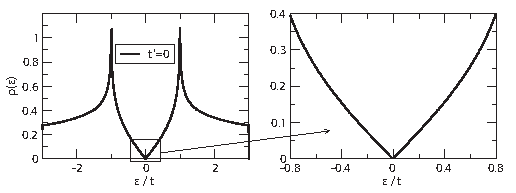
\includegraphics[width=.9\textwidth]{Drawing/DOS.pdf}
	\caption{The density of state of graphene near the Dirac point, assuming the hopping energy between the second nearest neighbor $t'$ is zero. $\epsilon$ is the Fermi energy, $t$ is the hopping energy in the tight binding model. Adapted from \cite{neto2009electronic}.}
	\label{FIG:DOS}
\end{figure}

\begin{figure}[h!]
	\centering
	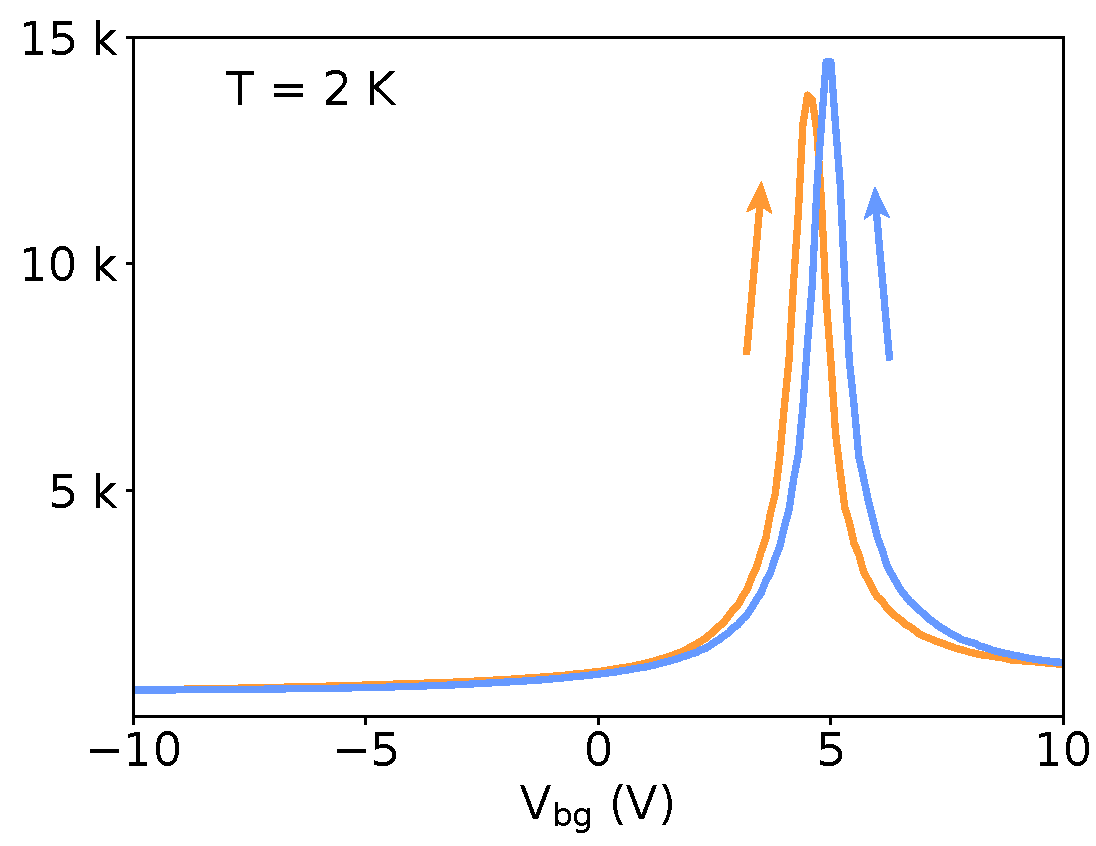
\includegraphics[width=.6\textwidth]{Drawing/DiracPeak.pdf}
	\caption{Graphene resistance as a function of backgate voltage. The resistance shows a maximum when the chemical potential reaches the CNP. The positions of the CNP are different for forward and backward sweeps. The arrows indicate the directions of sweeping. Measured at $T = 2$ K.}
	\label{FIG:DiracPeak}
\end{figure}

The effect of STO dielectric constant change as the temperature changes is critical for graphene devices on LAO/STO, as discussed in literatures\cite{couto2011transport}. Figure \ref{FIG:ResistanceTemp} demonstrates the change of resistance as a function of $V_\mathrm{bg}$. As the temperature drops, the dielectric constant of STO increase from 300 to 20,000, about two order of magnitude. Therefore the effective gating range under the same backgate sweeping range ($-15$ V to $+15$ V in this figure) also drastically increases. Therefore, at low temperature ($T < 10$ K) gating through 1 mm of STO is still effective.

Another effect of LAO/STO substrate is the hysteresis behavior under backgate sweeping. The position of CNP on $V_\mathrm{bg}$ shifts after each backgate voltage sweep. Although STO is not ferroelectric material, the dipole moment induced by displacement of oxygen atoms would result in ferroelectric-like hysteresis behavior\cite{sachs2014ferroelectric}. Similar hysteresis behavior has been reported elsewhere\cite{jnawali2017room}. The position of CNP has been a widely used indication for the quality of graphene on other substrates like SiO$_2$ or hBN. Graphene doping level is directly related to the contaminant on substrates as dopant, and therefore high quality graphene on these substrates have CNP very close to $V_\mathrm{bg} = 0$ V. For graphene on LAO/STO however, the position of CNP is usually at the positive side, even when the quality of graphene is comparable or better than those on SiO$_2$ substrates. 
\\

\begin{figure}[h!]
	\centering
	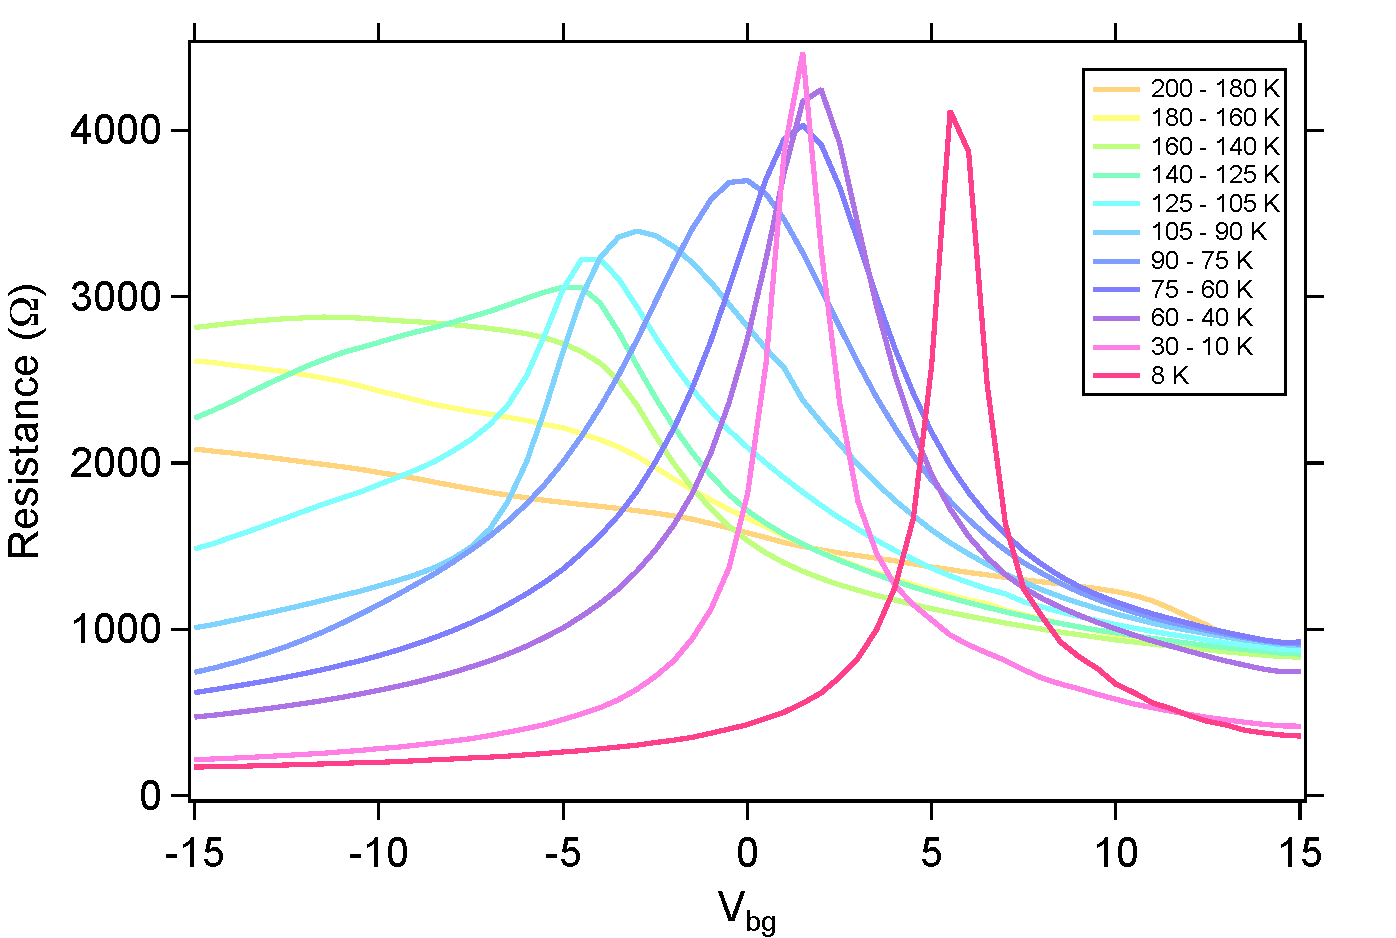
\includegraphics[width=.8\textwidth]{Drawing/ResistanceTemp.pdf}
	\caption{Resistance as a function of $V_\mathrm{bg}$ sweep at different temperatures. The width of the CNP clearly shows the change of dielectric constant of STO as a function of temperature.}
	\label{FIG:ResistanceTemp}
\end{figure}

\subsection{Carrier densities and mobilities}

The carrier density and mobility of graphene can be measured from Hall effect, using equation \ref{EQN:Hall}. From Figure \ref{FIG:CarrierDensityMobility} it can be seen that the high dielectric constant of STO at low temperature enables graphene gating to up to $1 \times 10^{13}$ $\mathrm{cm}^{-2}$ on the hole side (not shown in the Figure). On the electron side, due to the 2DEG electron gas induced by the high backgate voltage, the gating effect on graphene is shielded, and the carrier density usually saturates at about $n = 1 \times 10^{12}$ $\mathrm{cm}^{-2}$. Close to the CNP the carrier density and mobility are not well defined due to the existence of electron-hole puddles. Although it was believed that the high dielectric constant of STO can shield off the scattering effect charge impurity and improve the graphene mobility, the existence of surface dipole reduces the shielding effect\cite{sachs2014ferroelectric}. In spite of this, the Hyflon transfer method followed by contact AFM cleaning leaves the graphene on LAO/STO with high quality. The mobility of graphene reach $30,000$ cm$^{2}$V$^{-1}$s$^{-1}$, higher than most of the graphene on SiO$_2$ substrates. 
\\

\begin{figure}[h!]
	\centering
	\includegraphics[width=.7\textwidth]{Drawing/CarrierDensityMobility.pdf}
	\caption{Carrier density and mobility of graphene measured from Hall effect. The high dielectric constant makes it possible for the backgate to tune the graphene to a high carrier density on the hole side. However, the tuning effect saturate on the electron side due to the shielding of 2DEG induced on the interface. The carrier density is not well defined close to the CNP, due to the existence of electron-hole puddles. The quality of graphene is higher than most of the CVD graphene transferred on SiO$_2$, and the mobility can reach 30,000 cm$^2$V$^{-1}$s$^{-1}$.}
	\label{FIG:CarrierDensityMobility}
\end{figure}

\subsection{Quantum Hall effect}

As discussed in Section \ref{SEC:QuantumHall}, single layer graphene has unique half integer filling factor with degeneracy $N = 4$ from spin and valley pseudo-spin. The Hall conductance is
$$
\sigma_{xy} = \pm 4\left(n + \frac{1}{2}\right)\frac{e^2}{h}.
$$
in quantum Hall regime. The longitudinal resistance is suppressed except when the Fermi energy is transiting between Landau levels, and the localized states start to be filled. Figure \ref{FIG:HallResistance} demonstrate the longitudinal and transverse resistance of graphene device in a magnetic field of $B = 5$ T. The blue line is the Hall resistance that shows quantum Hall effect plateaus, with the filling factor $\nu$ marked by the numbers. The red line is the longitudinal resistance, that shows non-zero resistance at the transition energy between Landau levels.
\\

\begin{figure}[h!]
	\centering
	\includegraphics[width=.7\textwidth]{Drawing/HallResistance.pdf}
	\caption{Integer quantum Hall effect of single layer graphene.}
	\label{FIG:HallResistance}
\end{figure}

\section{Graphene p-n junction edge-state engineering}

In this section, the experiment of using c-AFM to dope the graphene into $p$-$n$ junction to reversibly engineer the edge state mixing is discussed.

\subsection{1D waveguide and quantum Hall edge channels}

In semi-classical point of view, the electrons under high magnetic field would cycle in the 2DEG and bounce back from the edges or scattering centers. If the scattering center is far from the edge, the electrons would cycle around the scattering centers and trapped in the localized state. If the scattering centers are close to the edge, the electrons would then collide with the edge and keep moving in the same direction. Therefore, chiral edge channels are formed with back scattering being suppressed. The transport of the edge state in the quantum Hall regime can be quantified with Landauer-B{\"u}ttiker formalism for 1D waveguides\cite{buttiker1986four, buttiker1988absence}.
\\

\begin{figure}[h!]
	\centering
	\includegraphics[width=.5\textwidth]{Drawing/Channel.pdf}
	\caption{Conductor channel connecting two reservoirs. The chemical potential of the two reservoirs are $\mu_1$ and $\mu_2$. The shaded region introduces elastic scatterings.}
	\label{FIG:Channel}
\end{figure}

Consider a strip on $x$-$y$ plane, as shown in Figure \ref{FIG:Channel}. The Hamiltonian is
$$
H = \frac{1}{2m}\left(p_x^2 + P_y^2\right) + V(y)
$$ 
$x$ is along the direction of the strip and $y$ is transverse to the strip. The wavefunction can be separated into the form
$$
\psi_{j, k}(x, y) = e^{ikx} f_j(y),
$$
$k$ is the wave vector along the $x$ direction, and $f_j(y)$ is the eigenfunction in $y$ direction with energy $E_j$. The Fermi energy is 
$$
E_F = E_j + \frac{\hbar^2 k_j^2}{2m}
$$
which is the sum of longitudinal and transverse energies, with 2$N$ state, where $N$ is the number of transverse energy levels $E_j$ below $E_F$. $\mu_1$ and $\mu_2$ are the chemical potentials of the two reservoirs, with $\mu_1 > \mu_2$. Only energy between $\mu_1$ and $\mu_2$ contribute to the current flowing from left to right. The current in channel $j$ is 
$$
I_j = \frac{dn}{dE_j}ev_j\Delta\mu,
$$
with 
$$
v_j = \frac{1}{\hbar}\frac{dE_j}{dk}, \ \ \ \Delta \mu = \mu_1 - \mu_2
$$
and $v_j$ being the velocity along channel $j$. In one dimension, density of state
$$
\frac{dn}{dk} = \frac{1}{2\pi},
$$
and therefore the current in channel $j$ is
$$
I_j = \frac{e}{h}\Delta\mu.
$$
The current for all $N$ channels is
$$I = N\frac{e}{h}\Delta\mu.$$
Using the voltage drop $\Delta \mu = eV$ and Ohm's law, the resistance of the conductor with $N$ channels is
$$
R = \frac{h}{e^2}\frac{1}{N}
$$ 
which is quantized. Consider there elastic scattering that redistributing energies between the $N$ channels, the resistance becomes\cite{buttiker1988absence}
$$
R = \frac{h}{e^2}\frac{1}{T}
$$
$T = \sum_{i,j=1\ldots N} T_{ij}$, and $T_{ij}$ is the transmission probability from channel $j$ into channel $i$. 

\subsection{Edge channel mixing of graphene unipolar/bipolar junction in quantum Hall regime}

In the quantum Hall regime, edge channels of graphene can be described by the Landauer-B{\"u}ttiker formalism. When two adjacent regions of graphene have different carrier density and Landau level filling factors in magnetic field, the numbers or directions of channels will be different which would cause channel mixing. In Figure \ref{FIG:Mixing}(a), the two adjacent regions have different carrier densities, and therefore the filling factors and number of edge channels for the two regions are different. The edge currents flow in the same direction (unipolar, but part of the current would be reflected into the interface of the two regions. In Figure \ref{FIG:Mixing}(b), the two regions have opposite carrier types, and the directions of edge currents are the opposite (bipolar). The edge channels would mix on the interface. In both cases, the longitudinal resistance is non-trivial as a result of channel mixing.

\begin{figure}[h!]
	\centering
	\includegraphics[width=.4\textwidth]{Drawing/Mixing.pdf}
	\caption{(a) Two regions with the same carrier type but the region on the left hand side has more edge channels than the right hand side. The currents are flowing in the same directions but part of the current would be reflected on the interface of the two regions. (b) Two regions with different carrier types. The currents flow in opposite directions in the two regions, and would mix on the interface of the two regions.}
	\label{FIG:Mixing}
\end{figure}

For the unipolar case, as shown in Figure \ref{FIG:Unipolar}, assume the current is sourced from the left and $\mu_L > \mu_R$. Filling factors $|\nu_1| > |\nu_2|$ and the currents are flowing clock-wise (same as Figure \ref{FIG:Mixing}(a)). The chemical potential of the four voltage leads are $\mu_A$, $\mu_B$, $\mu_C$ and $\mu_D$. $I_1$ to $I_8$ are the currents flowing between the current and voltage leads:
\begin{equation}
\label{EQN:MixCurr1}
	\begin{split}
		I_1 & = \frac{e}{h}\mu_L|\nu_1|, \ \ \ \  I_2 = \frac{e}{h}\mu_A|\nu_1|, \\
		I_3 & = I_2 - I_M, \ \ \ \ I_4 = \frac{e}{h}\mu_B|\nu_2| \\
		I_5 & = \frac{e}{h}\mu_C|\nu_1|, \ \ \ \ I_6 = I_M + I_7 \\
		I_7 & = \frac{e}{h}\mu_D|\nu_2|, \ \ \ \ I_8 = \frac{e}{h}\mu_R|\nu_2|
	\end{split}
\end{equation}

The region on the left hand side has more channels, and therefore the excessive current is reflected into the interface and $I_M = \frac{e}{h}\mu_L(|\nu_1|-|\nu_2|)$. The net currents flowing into and out of the four voltages leads are zero, i.e.
$$
I_1 = I_2, \ \ I_3 = I_4, \ \ I_5 = I_6, \ \ I_7 = I_8
$$
and therefore the chemical potentials of the four leads are
\begin{equation}
\label{EQN:MixMu1}
\mu_A = \mu_B = \mu_L, \ \ \mu_C = \mu_L + \frac{|\nu_2|}{|\nu_1|}(\mu_L - \mu_R), \ \ \mu_D = \mu_R.
\end{equation}
From equation \ref{EQN:MixCurr1} and \ref{EQN:MixMu1}, the total current from left to right is 
$$
I = I_1 - I_5 = \frac{e}{h}(\mu_L - \mu_R)|\nu_1|,
$$ 
and the longitudinal resistances are 
\begin{equation}
\label{EQN:Mixing1}
\begin{split}
R_{AB} & = \frac{\mu_A - \mu_B}{eI} = 0, \\
R_{CD} & = \frac{\mu_C - \mu_D}{eI} = \frac{h}{e^2}\left(\frac{1}{|\nu_2|} - \frac{1}{|\nu_1|}\right).
\end{split}
\end{equation}
\\

\begin{figure}[h!]
	\centering
	\includegraphics[width=.7\textwidth]{Drawing/Unipolar.pdf}
	\caption{Edge currents of the unipolar junction.}
	\label{FIG:Unipolar}
\end{figure}

For the bipolar case, as shown in Figure \ref{FIG:Bipolar}, again assume that the chemical potentials $\mu_L > \mu_R$. The two regions have different carrier type and the currents are flowing in the opposite directions. The channels are mixed at the interface, and therefore $I_M$ is equal to the sum of currents from each side, and then redistributed into edge channels on the bottom. Therefore the edge currents are
\begin{equation}
\label{EQN:MixCurr2}
\begin{split}
I_1 = \frac{e}{h}\mu_L|\nu_1|, & \ \ \ \   I_2 = \frac{e}{h}\mu_A|\nu_1|, \\
I_3 = \frac{e}{h}\mu_B|\nu_2|, & \ \ \ \ I_4 = \frac{e}{h}\mu_R|\nu_2| \\
I_5 = \frac{e}{h}\mu_C|\nu_1|, & \ \ \ \  I_6 = \frac{|\nu_1|}{|\nu_1|+|\nu_2|} \cdot I_M \\
I_7 = \frac{|\nu_2|}{|\nu_1|+|\nu_2|} \cdot I_M, & \ \ \ \ I_8 = \frac{e}{h}\mu_D|\nu_2|,
\end{split}
\end{equation}
with $I_M = I_2 + I_3$. The net currents flowing into and out of the four voltages leads are zero, i.e.
$$
I_1 = I_2, \ \ I_3 = I_4, \ \ I_5 = I_6, \ \ I_7 = I_8
$$
and therefore the chemical potentials of the four leads are
\begin{equation}
\label{EQN:MixMu2}
\mu_A = \mu_L, \ \ \mu_B = \mu_R, \ \ \mu_C = \mu_D = \frac{\mu_L|\nu_1| + \mu_R|\nu_2|}{|\nu_1| + |\nu_2|}.
\end{equation}
From equation \ref{EQN:MixCurr2} and \ref{EQN:MixMu2}, the total current from left to right is 
$$
I = I_1 - I_5 = \frac{e}{h} \cdot \frac{|\nu_1||\nu_2|}{|\nu_1| + |\nu_2|} \cdot (\mu_L - \mu_R),
$$ 
and the longitudinal resistances are 
\begin{equation}
\label{EQN:Mixing2}
\begin{split}
R_{AB} & = \frac{\mu_A - \mu_B}{eI} = \frac{h}{e^2}\left(\frac{1}{|\nu_1|} + \frac{1}{|\nu_2|}\right), \\
R_{CD} & = \frac{\mu_C - \mu_D}{eI} = 0.
\end{split}
\end{equation}
\\

\begin{figure}[h!]
	\centering
	\includegraphics[width=.7\textwidth]{Drawing/Bipolar.pdf}
	\caption{Edge currents of the bipolar junction.}
	\label{FIG:Bipolar}
\end{figure}

\subsection{Graphene doping using c-AFM}

There have been efforts to locally control the CNP of graphene on silicon or hBN substrates using AFM\cite{schmidt2013mixing} or STM\cite{velasco2016nanoscale}. However, those doping techniques are either non-reversible, or can only be performed in ulrtra-high vacuum and low temperature, which limits the applications. In this work, we demonstrate how local control over the metal-insulator transition in LAO/STO can be used to reversibly pattern interacting edge channels in a proximal graphene layer under ambient conditions. The CNP of graphene can be locally shifted by c-AFM tip with positive bias voltage. Therefore, c-AFM writing can be used to selectively dope graphene regions and engineer edge state mixing in quantum Hall regime.

The mechanism of using c-AFM to locally shift the CNP is similar to c-AFM nanostructure lithography technique discussed in section \ref{SEC:AFMLitho}. As Figure \ref{FIG:GrapheneAFM} shows, when a positively biased tip in scanning the graphene in contact mode while the graphene is grounded, a trace of protons will be left on graphene, and permeate\cite{hu2014proton} to the interface between graphene and LAO. The proton would locally dope the graphene and shift the CNP. 
\\

\begin{figure}[h!]
	\centering
	\includegraphics[width=.45\textwidth]{Drawing/GrapheneAFM.pdf}
	\caption{Graphene doping using c-AFM writing technique. A trace of proton would be left by the tip and permeate to the interface of graphene and LAO. The voltage of back gate is kept at zero during c-AFM writing.}
	\label{FIG:GrapheneAFM}
\end{figure}

One common method of monitoring the doping level of graphene is to sweep the back-gate voltage and compare the position of CNP before and after the doping. The method cannot be used for graphene on LAO/STO substrates for two reasons: (1) the surface of LAO is not charge neutral, and therefore the CNP is not at $V_\mathrm{bg}$ is not at 0 V even without c-AFM doping; (2) the $V_\mathrm{bg}$ is subject to significant hysteresis\cite{couto2011transport, jnawali2017room} (also shown in Figure \ref{FIG:DiracPeak}) and is not a reliable indicator of doping level with respect to CNP. Instead, the four-terminal resistance of graphene is measured \emph{in situ} to monitor the doping level change during the c-AFM writing process. 

In Figure \ref{FIG:WritingResistance}, a graphene device is scanned with c-AFM with a tip voltage of $V_\mathrm{tip} = +17$ V continuously. The scanned region covers the entire device, as shown in the inset of the figure. The current flows from left to right, and the longitudinal resistance is measured as a function of time as the scanning proceeds. At $t$ = 0 s, the graphene is $n$-type doped. The AFM scanning speed is 10 $\mu$m/s, and it takes 260 s to scan the graphene device (5 $\mu$m $\times$ 10 $\mu$m). 15 consecutive scans are recorded. Blue dots mark the beginning/ending of the consecutive AFM raster scans. The positive charges left by c-AFM scans increase the local doping level and drives the chemical potential away from the CNP and further into the $n$-type region (illustrated by the Dirac cone in the inset). Within each scan, the resistance decreases at the beginning due to the doping, and then start to recover when the scan is half finished. The green region marks one complete scan. The resistance recovery speed is observed to be related to the environmental humidity, and is possibly caused by the recombination of protons with water molecules in the air. The terminal resistance after each scan (marked by the blue dots) decreases as the scan proceeds, indicating that the $n$-type doping level of graphene is increasing as the scan proceeds.
\\

\begin{figure}[h!]
	\centering
	\includegraphics[width=1\textwidth]{Drawing/WritingResistance.pdf}
	\caption{Monitoring the doping level change during c-AFM writing process. The rectangle region in the inset is scanned with c-AFM tip continuously, while the four-terminal resistance is measured. The blue dots mark the beginning/ending of the consecutive scans. The green region marks one complete scan. The resistance drop in the first half of each scan, and then recover as the scan proceeds. The terminal resistance of each scan decreases as the scan proceeds, indicating increasing $n$-type doping level of graphene.}
	\label{FIG:WritingResistance}
\end{figure}

The graphene doping from the positively biased c-AFM tip is reversible. After the c-AFM writing and the change in four-terminal resistance being observed, a scan with $V_\mathrm{tip}= -5$ V voltage on the c-AFM tip will partially remove the previous writing effect. Scans with negative $V_\mathrm{tip}$ need to be carefully conducted and the c-AFM tip should be connected in series with a 1 G$\Omega$ resistor, due to the fact that graphene can be oxidized as anode\cite{alaboson2011conductive, byun2011nanoscale}. Also, graphene has to be detached from measurement leads or groundings so that there is no significant current flowing through graphene\cite{alaboson2011conductive}. 

\subsection{Measurement of graphene edge state mixing}

The edge state mixing engineering can be achieved by doping graphene regions with c-AFM writing technique. In Figure \ref{FIG:GrapheneDopedHall}, the right-hand-side region of the graphene device is written with c-AFM tip and locally doped with positive charges. Carrier densities measured on the two pairs of Hall electrodes (Hall A and Hall B) indicate that the CNP for the written area (B) is shifted to the left.
\\

\begin{figure}[h!]
	\centering
	\includegraphics[width=.7\textwidth]{Drawing/GrapheneDopedHall.pdf}
	\caption{Carrier density of locally doped graphene. Carrier densities of the two pairs of Hall electrodes (Hall A and Hall B) are measured at $T = 2$ K. The CNP of the written region (B) is shifted to the left, indicating the doping effect of positive charges.}
	\label{FIG:GrapheneDopedHall}
\end{figure}

The longitudinal resistance (as shown in the inset of Figure \ref{FIG:GrapheneDopedHall}) is also measured as a function of $V_\mathrm{bg}$ to indicate the effect of c-AFM writing. Figure \ref{FIG:DiracPointSplit}(a) is the resistance measured before c-AFM writing, and a single Dirac peak can be seen. Figure \ref{FIG:DiracPointSplit}(b) is measured after the writing, and a second Dirac peak is distinguishable. The peak on the left hand side is correspond to the written area (B in the inset of Figure \ref{FIG:GrapheneDopedHall}).
\\

\begin{figure}[h!]
	\centering
	\includegraphics[width=.75\textwidth]{Drawing/DiracPointSplit.pdf}
	\caption{Longitudinal resistance as a function as $V_\mathrm{bg}$. (a) is measured before c-AFM writing as a control measurement. Dirac peak is clearly visible. (b) is measured after c-AFM writing. Splitting of Dirac peak can be observed. The peak on the left hand side is correspond to the written area (shown in the inset of Figure \ref{FIG:GrapheneDopedHall}).}
	\label{FIG:DiracPointSplit}
\end{figure}

Graphene sample with half of the device written by c-AFM is then measured in magnetic field with $B = 7$ T. The longitudinal resistances are measured from the bottom ($R_\mathrm{xx1}$) and top ($R_\mathrm{xx2}$) pairs of electrodes as functions of $V_\mathrm{bg}$. The result is shown in Figure \ref{FIG:EdgeChannels}(a). $R_\mathrm{xx1}$ is quantized at $h/3e^2$ at around $V_\mathrm{bg} = 0$ V, then is suppressed between 1 V and 3 V, and then quantized at $h/3e^2$ again around $V_\mathrm{bg} = 5$ V. $R_\mathrm{xx2}$ is suppressed around $V_\mathrm{bg} = 0$ V and 5 V, and is quantized at $h/e^2$. 

Figure \ref{FIG:EdgeChannels}(b) is the zoomed-in plot of Figure \ref{FIG:GrapheneDopedHall} around the CNP. At line cut (I), both regions are $p$-type doped, as shown in the left sub-figure of (c). However, the two regions have different Landau level filling factors in magnetic field, and therefore the number of edge channels are different, although the currents are all flowing in clock-wise direction. The excessive currents from the left region are reflected into the interface in the middle, and then mixed with the currents from the right on the bottom. The channel mixing result in non-trivial longitudinal resistance and the values of $R_\mathrm{xx1}$ and $R_\mathrm{xx2}$ can be predicted with equation \ref{EQN:Mixing1}. At line cut (III), both regions are $n$-type dope, but again with different carrier densities and therefore different filling factors and number of edge channels in magnetic field. The longitudinal resistances can also be calculated using the same formalism. At line cut (II), the two regions have opposite carrier type, and the currents are flowing different directions and mixed on the interface in the middle (shown by the arrows in the middle sub-figure of \ref{FIG:GrapheneDopedHall}(c)). The quantized resistances can be calculated from equation \ref{EQN:Mixing2}.


\begin{figure}[p]
	\centering
	\includegraphics[width=1.0\textwidth]{Drawing/EdgeChannels.pdf}
	\caption{The edge channel mixing changes as $V_\mathrm{bg}$ is swept from $-10$ V to $+10$ V. (a) $R_\mathrm{xx1}$ and $R_\mathrm{xx2}$ are quantized at values predicted by equation \ref{EQN:Mixing1} and \ref{EQN:Mixing2}. (b) Zoomed-in plot of Figure \ref{FIG:GrapheneDopedHall}. (c) Filling factors and edge current directions of the three cases of edge state mixing.}
	\label{FIG:EdgeChannels}
\end{figure}

\begin{figure}[h!]
	\centering
	\includegraphics[width=1.0\textwidth]{Drawing/MixingIntensityPlot.pdf}
	\caption{Intensity plot of longitudinal resistance $R_\mathrm{xx1}$ and $R_\mathrm{xx2}$ as functions of $V_\mathrm{bg}$ and magnetic field sweep. The values of $R_\mathrm{xx1}$ and $R_\mathrm{xx2}$ are swapped when the direction of magnetic field is reversed.}
	\label{FIG:MixingIntensityPlot}
\end{figure}
 
When the magnetic field is reversed, the directions of current in all three cases are reversed. Therefore the values of $R_\mathrm{xx1}$ and $R_\mathrm{xx2}$ are swapped. To demonstrate the transition of longitudinal resistances when the direction of magnetic field is flipped, $R_\mathrm{xx1}$ and $R_\mathrm{xx2}$ are measured at magnetic fields from $-7$ T to $+7$ T, while $V_\mathrm{bg}$ is swept at each magnetic field step. Figure \ref{FIG:MixingIntensityPlot} is the intensity plot of $R_\mathrm{xx1}$ and $R_\mathrm{xx2}$ as functions of $V_\mathrm{bg}$ and $B$. In Figure \ref{FIG:MixingIntensityPlot}(a) $R_\mathrm{xx1}$ is clearly quantized at $h/3e^2 \approx 8.6 \ \mathrm{k}\Omega$ at $B = +7$ T. The quantization gradually disappears as $B$ gets close to 0. Then $R_\mathrm{xx1}$ start to be quantized at $h/e^2 \approx 25.8 \ \mathrm{k}\Omega$ when the field increases in the opposite direction. In Figure \ref{FIG:MixingIntensityPlot}(b) $R_\mathrm{xx1}$ shows the opposite behavior as the field is stepped from $-7$ T to $+7$ T. The observation of mixed edge channel is consistent with results reported elsewhere\cite{williams2007quantum, lohmann2009four, amet2014selective, abanin2007quantized, amet2014selective, ki2010dependence, klimov2015edge, woszczyna2011graphene, ozyilmaz2007electronic, schmidt2013mixing} and is the direct proof of doping effect of c-AFM writing on graphene.

\section{Graphene band structure engineering with superlattice}

\chapter{Magneto-Optical Kerr Effect on LAO/STO interface}
\label{SEC:Kerr}

This sections will discuss the experiment of probing ferromagnetism in LAO/STO using MFM and magneto-optical Kerr effect. 

\section{Magnetism on LAO/STO interface}

The signature magnetism on the interface of LAO/STO was first observed in the low temperature transport data by Brinkman et al in 2007\cite{brinkman2007magnetic}. Micron-scale magnetic dipole patches was later imaged using scanning SQUID\cite{bert2011direct, kalisky2012scanning, kalisky2012critical}. The origin of the magnetism is still controversial. X-ray dichroism (XMCD) signal indicates that the ferromagnetism is intrinsic and is linked to $d_{xy}$ orbitals of Ti$^{3+}$\cite{lee2013titanium}. Extrinsic sources of magnetic impurities have been ruled out experimentally\cite{brinkman2007magnetic, lee2013titanium, ariando2011electronic}. DFT calculation further suggests that the oxygen vacancies near the interface are possible source of localized magnetic moments\cite{pentcheva2006charge}. 

The LAO/STO interface magnetism is also discovered to be electronically tunable in room temperature from MFM measurement\cite{bi2014room}. The in-plane magnetism could only be detected when the electrons are depleted by a top-gate voltage. Reintroducing the itinerant electrons would screen and destabilize the interface magnetism, suggesting that itinerant carriers are critical for coupling localized unpaired $d_{xy}$ electron spins\cite{fidkowski2013magnetic, Joshua2013gate, banerjee2013ferromagnetic}. MFM has high sensitivity for magnetism, and the measurement can be performed in ambient conditions. However, as discussed in \ref{SEC:AFMMFM}, the signal is dependent on the spatial gradient of magnetic force. Therefore it would be challenging to perform time-resolved measurement. Observation of magnetic circular dichroism (MCD) signal in oxygen-deficit STO samples\cite{rice2014persistent} make it possible to use circularly polarized laser to detect magnetism in LAO/STO. By using pulsed laser for magneto-optical Kerr measurement, time-evolution of gate tunable magnetism in LAO/STO can be measured, so that the origin of magnetism in LAO/STO can be further investigated.

\begin{figure}[p]
	\centering
	\includegraphics[width=0.9\textwidth]{Drawing/MCDRice.jpg}
	\caption{MCD experiment on oxygen-deficit STO. (a) The schematics of the optical setup of MCD. (b) An additional peak at $\lambda=425$ nm is observed in the absorption spectra of the oxygen-deficit STO samples. (c) MCD spectra of oxygen-deficit and as-received samples after illuminated by circular and linearly polarized pump laser. (d) Temperature dependence of the MCD signal. (e) Temperature dependent magnetic signal measured by SQUID. Adapted from \cite{rice2014persistent}.}
	\label{FIG:MCDRice}
\end{figure}

Similar to magneto-optical Kerr measurement, MCD also utilize the broken time-reversal symmetry to measure magnetism. The experimental setup and results of MCD on oxygen-deficit STO samples are shown in Figure \ref{FIG:MCDRice}. The sample is loaded in a cryostat with variable temperature from 1.7 K to 300 K. The magnetism is induced by a circularly polarized pump laser (circularly polarized laser through a quarter wave plate). Continuous wave probe laser is modulated between left- and right-circularly polarized by a linear polarizer and a photo-elastic modulator (PEM). The probe laser transmits through the sample and is then detected by an avalanche photo-detector for MCD signal (as shown in Figure \ref{FIG:MCDRice}(a)). For the At $T = 3$ K, an additional peak can be observed around $\lambda = 425$ nm in the absorption spectra for the oxygen-deficit samples(Figure \ref{FIG:MCDRice}(b)). Around the absorption peak, oscillatory MCD signal can be measured as a function of wavelength of probe laser while pump laser wavelength is fixed at $\lambda_{\mathrm{pump}} = 405$ nm, suggesting pump-induced magnetism (Figure \ref{FIG:MCDRice}(c)). Figure \ref{FIG:MCDRice}(d, e) shows the temperature dependence of magnetic signal measured with MCD and SQUID, suggesting that the magnetism in the oxygen-deficit STO sample appears only at $T < 18$ K. The MCD signal suggests that the magnetism in STO is related to oxygen-vacancy complex and also proves that it is possible to use optical method to probe magnetism in LAO/STO. In this section I will discuss the experimental details of using magneto-optical Kerr effect of circularly polarized laser to detect LAO/STO interface magnetism.

\section{MFM measurement}

\begin{figure}[p]
	\centering
	\includegraphics[width=1.0\textwidth]{Drawing/LAOSTOMFM.pdf}
	\caption{(a) MFM experiment setup. The sample within ferromagnetism thickness window of LAO (8 u.c. to 25 u.c.) is patterned with a top gate electrode and interface electrode. The top gate is connected with the conductive MFM tip and grounded. The interface and top gate form a capacitor. A positive voltage of $+1$ V to $+3$ V is applied to the interface and the interface electrons are depleted. The MFM tip coated with 50 nm of Co/Fe alloy is magnetized in the in-plane direction. When the itinerant electrons are depleted by gate voltages, the ferromagnetism is visible from MFM measurements. (b) and (c) are the capacitance and leakage current between the interface and top gate, as functions of relative voltage between the interface electrode and top gate. The top-gate voltage in the figures is equal to the potential on the top gate (grounded) minus the potential on the interface. When the top-gate voltage is lower than $-0.5$ V, both the capacitance and leakage are close to zero, meaning the interface carriers are depleted.}
	\label{FIG:LAOSTOMFM}
\end{figure}

In spite of the limitation of MFM, it is proved to be a technique with highly sensitivity\cite{bi2014room} for magnetism detection, and therefore I used it for sample screening before the magneto-optical Kerr experiment was performed. The experimental setup is shown in Figure \ref{FIG:LAOSTOMFM}. An LAO/STO sample within ferromagnetism  thickness window (8 u.c. to 25 u.c.) of LAO\cite{bi2015laalo3} is patterned with an interface electrodes and top electrodes. The thickness of LAO is greater than the critical thickness for 2DEG formation, and therefore the interface is conductive when the gate voltages is zero. The interface and top gate form a capacitor, and the capacitance depends on the carrier concentration on the interface. By applying a voltage between the top gate and interface, the carriers can be depleted. As shown in Figure \ref{FIG:LAOSTOMFM}(b) and (c), the capacitance and leakage current is measured as functions of top-gate voltage, the potential difference between the top gate and the interface $V_\mathrm{tg} = \phi_\mathrm{tg} - \phi_\mathrm{int}$. When $V_\mathrm{tg} < -0.5$ V, both the capacitance and leakage current are close to zero as the electrons are depleted. The magnetism is measured with an MFM tip magnetized in the in-plane direction, when $V_\mathrm{tg} < -0.5$ V. In practice, the MFM tip and the top gates are both grounded, and a positive voltage is applied to the interface to deplete the electrons under the top gate, so that the electrical potential would not be coupled to the MFM signal. Figure \ref{FIG:MFMSignal} shows the optical image (left) of an MFM device on LAO/STO and the magnetic signal from MFM scan. The diagonal strips are ferromagnetic domains on the interface of LAO/STO.
\\

\begin{figure}[h!]
	\centering
	\includegraphics[width=0.8\textwidth]{Drawing/MFMSignal.pdf}
	\caption{Optical image of the MFM device and MFM signal for interface magnetism. The circular shape region is the top gate, and the arc-shape electrode is the interface electrode. MFM image is scanned on a 30 $\mu$m $
		\times$ 30 $\mu$m region on the top gate while the electrons are depleted. Diagonal strips are visible in the MFM image.}
	\label{FIG:MFMSignal}
\end{figure}


\section{Magneto-Optical Kerr measurement}

The samples having MFM signal are used for magneto-Optical Kerr measurement. In this section, principles of measurement is derived using Jone's matrix formalism. Optical setup and measurement results are also discussed.

\subsection{Jone's matrix formalism}

The Jone's matrix is used for describing polarized light.

\subsection{Optical measurement}

\chapter{Conclusions}

\chapter{Outlook}


%
\appendix                          % After this command, chapters will be formatted as appendices. For example:
%
\bibliography{bibliography}      %\safebibliography is used the same way as \bibliography, but gives pittetd
\bibliographystyle{unsrt}
%                                   a greater chance to succeed in formatting the bibliography when non-standard
% 

                                  %BibTeX styles are used.
\end{document}
